\documentclass[10pt,a4paper]{article}
\usepackage[utf8]{inputenc}
\usepackage[T1]{fontenc}
\usepackage[polish]{babel}
\usepackage[margin=1in]{geometry}
\usepackage{amsmath}
\usepackage{amsfonts}
\usepackage{amssymb}
\usepackage{dirtytalk}
\usepackage{color}
\usepackage{float}
\usepackage{hyperref}

\hypersetup{colorlinks=true, urlcolor=blue}

%\usepackage[pdftex,
%            pdfauthor={Andrzej Roguski},
%            pdftitle={Techniki Internetowe, Projekt}]{hyperref}
            
\usepackage{graphicx}

\graphicspath{{./images/}}

\title{Low Orbit Task Cannon \\ \large Techniki Internetowe, Projekt \\ \\ Dokumentacja końcowa}
\date{\today}
\author{Tomasz Jakubczyk, Eryk Ratyński, Andrzej Roguski, Kacper Stachyra}

\begin{document}
	\maketitle
	
	\begin{flushright}
	    \href
	    {https://github.com/sigrond/procesy_rozproszone}
	    {\underline{Low Orbit Task Cannon na serwerze GitHub}}
	\end{flushright}
	
	\section{Treść zadania}
	    \say{W sieci jest zbiór zarządzanych węzłów, serwer zarządzający i stacja konsoli administratora. W węzłach pracują agenty zarządzające. Agent zarządzający może: załadować kod nowego procesu, usunąć kod procesu, uruchomić/zatrzymać/wznowić/zabić dany proces zgodnie z harmonogramem, wznowić proces nie raportujący swej żywotności, podać dane statystyczne serwerowi. System umożliwia administratorowi zarządzanie rozproszonymi procesami. System komunikacji powinien móc pracować w przestrzeni adresów IPv4 i IPv6. Ponadto należy zaprojektować moduł do Wireshark umożliwiający wyświetlanie i analizę zdefiniowanych komunikatów.} \\
	
	\section{Założenia projektowe}
	    \subsection{Środowisko}
	
		\begin{itemize}
	        \item Low Orbit Task Cannon (LOTC) uruchamiany jest na systemie operacyjnym GNU/Linux
	        \item Hosty systemu LOTC mają działającą usługę synchronizacji czasu 
	    \end{itemize}
	    
	    \subsection{Zadania}
	    \begin{itemize}
	        \item Zadania po wprowadzeniu do LOTC nie wymagają modyfikacji
	        \item Wykonanie zadania wymaga uruchomienia wyłącznie jednego pliku wykonywalnego (może on jednak uruchamiać inne podprogramy)
	        \item Zadania dają się uruchomić w systemie GNU/Linux bez GUI (w szczególności - bez X Window System)
	        \item Zadania wykonywane są w trybie wsadowym, tj. nie wymagają interakcji z użytkownikiem
        \end{itemize}
        
	\section{Struktura systemu}
	
	    \subsection{Moduły}	
	        \paragraph{}
		    Low Orbit Task Cannon zawiera następujące moduły:
		
			\begin{enumerate}
		        \item Protokół LOTC
		        \item Serwer
		        \item Klient (agent)
		        \item Konsola administratora
		    \end{enumerate}
		    
	    \subsection{Topologia}
	    
		    \begin{itemize}
		        \item Każdy klient LOTC musi być połączony siecią TCP/IP z serwerem LOTC
		        \item Konsola administratora musi być połączona siecią TCP/IP z serwerem LOTC 
		        \item Serwer LOTC musi być połączony siecią TCP/IP
		    \end{itemize}
		    
		    \begin{figure}[H]
				\def\svgwidth{\columnwidth}
				\input{./images/Topology.pdf_tex}
			\end{figure}
			
        \pagebreak			
			
	    \subsection{Diagram rozmieszczenia}
		    Komunikacja między konsolą i serwerem oraz serwerem i klientem odbywa się poprzez protokół LOTC. Wykorzystywany jest do tego moduł implementujący protokół LOTC i wystawiający interfejs komunikacyjny. \\
		    Z racji potrzeby synchronizacji, serwer oraz klient wykorzystują moduł implementujący niezbędne minimum klienta NTP potrzebne do zapytania serwera NTP o aktualny czas. \\
		    Program do administracji zadaniami wystawia interfejs niezbędny do zbudowania UI, zarówno w wersji tekstowej jak i graficznej. \\

		    
		    \begin{figure}[H]
				\def\svgwidth{\columnwidth}
				%LaTeX with PSTricks extensions
%%Creator: inkscape 0.91
%%Please note this file requires PSTricks extensions
\psset{xunit=.5pt,yunit=.5pt,runit=.5pt}
\begin{pspicture}(492,321)
{
\newrgbcolor{curcolor}{1 1 1}
\pscustom[linestyle=none,fillstyle=solid,fillcolor=curcolor]
{
\newpath
\moveto(305.71,319.5)
\lineto(305.71,75.9)
\lineto(295.71,65.9)
\lineto(179.43,65.9)
\lineto(179.43,309.5)
\lineto(189.43,319.5)
\lineto(305.71,319.5)
\closepath
}
}
{
\newrgbcolor{curcolor}{0 0 0}
\pscustom[linewidth=1,linecolor=curcolor]
{
\newpath
\moveto(305.71,319.5)
\lineto(305.71,75.9)
\lineto(295.71,65.9)
\lineto(179.43,65.9)
\lineto(179.43,309.5)
\lineto(189.43,319.5)
\lineto(305.71,319.5)
\closepath
}
}
{
\newrgbcolor{curcolor}{0 0 0}
\pscustom[linewidth=1,linecolor=curcolor]
{
\newpath
\moveto(179.43,309.5)
\lineto(295.71,309.5)
\lineto(305.71,319.5)
\moveto(295.71,309.5)
\lineto(295.71,65.9)
}
}
{
\newrgbcolor{curcolor}{0 0 0}
\pscustom[linestyle=none,fillstyle=solid,fillcolor=curcolor]
{
\newpath
\moveto(213.21597188,293.32399969)
\curveto(213.21597188,292.7022549)(212.9913625,292.21234604)(212.54214375,291.85427313)
\curveto(212.092925,291.49620021)(211.467925,291.31716375)(210.66714375,291.31716375)
\curveto(209.82078958,291.31716375)(209.16649271,291.42946844)(208.70425313,291.65407781)
\lineto(208.70425313,292.51345281)
\curveto(209.0069875,292.38324448)(209.33739115,292.28070542)(209.69546406,292.20583563)
\curveto(210.05679219,292.13096583)(210.39370625,292.09353094)(210.70620625,292.09353094)
\curveto(211.24006042,292.09353094)(211.64207865,292.19607)(211.91226094,292.40114813)
\curveto(212.18244323,292.60622625)(212.31753438,292.88780177)(212.31753438,293.24587469)
\curveto(212.31753438,293.4835049)(212.26870625,293.6788174)(212.17105,293.83181219)
\curveto(212.07339375,293.98480698)(211.90900573,294.12803615)(211.67788594,294.26149969)
\curveto(211.45002135,294.39496323)(211.10334167,294.54633042)(210.63784688,294.71560125)
\curveto(209.97703958,294.95648667)(209.50503438,295.23968979)(209.22183125,295.56521063)
\curveto(208.93862813,295.89398667)(208.79702656,296.31716375)(208.79702656,296.83474188)
\curveto(208.79702656,297.3913825)(209.0053599,297.83409083)(209.42202656,298.16286688)
\curveto(209.84194844,298.49164292)(210.39370625,298.65603094)(211.0773,298.65603094)
\curveto(211.79019063,298.65603094)(212.4461151,298.5225674)(213.04507344,298.25564031)
\lineto(212.76675313,297.48415594)
\curveto(212.15477396,297.73806219)(211.5851125,297.86501531)(211.05776875,297.86501531)
\curveto(210.63459167,297.86501531)(210.30256042,297.77386948)(210.061675,297.59157781)
\curveto(209.82404479,297.40928615)(209.70522969,297.15375229)(209.70522969,296.82497625)
\curveto(209.70522969,296.59060125)(209.7508026,296.39528875)(209.84194844,296.23903875)
\curveto(209.93634948,296.08604396)(210.08608906,295.94607)(210.29116719,295.81911688)
\curveto(210.49950052,295.69216375)(210.82502135,295.54730698)(211.26772969,295.38454656)
\curveto(211.79832865,295.18923406)(212.19383646,294.99880438)(212.45425313,294.8132575)
\curveto(212.71466979,294.63096583)(212.90672708,294.41937729)(213.030425,294.17849188)
\curveto(213.15412292,293.94086167)(213.21597188,293.65603094)(213.21597188,293.32399969)
\closepath
}
}
{
\newrgbcolor{curcolor}{0 0 0}
\pscustom[linestyle=none,fillstyle=solid,fillcolor=curcolor]
{
\newpath
\moveto(216.81460469,291.31716375)
\curveto(216.01056823,291.31716375)(215.37905781,291.55967677)(214.92007344,292.04470281)
\curveto(214.46434427,292.53298406)(214.23647969,293.20355698)(214.23647969,294.05642156)
\curveto(214.23647969,294.91579656)(214.44969583,295.59939031)(214.87612813,296.10720281)
\curveto(215.30256042,296.61827052)(215.87873229,296.87380438)(216.60464375,296.87380438)
\curveto(217.27847188,296.87380438)(217.81558125,296.65570542)(218.21597188,296.2195075)
\curveto(218.6163625,295.78656479)(218.81655781,295.19899969)(218.81655781,294.45681219)
\lineto(218.81655781,293.92458563)
\lineto(215.14468281,293.92458563)
\curveto(215.16095885,293.31586167)(215.31558125,292.85362208)(215.60855,292.53786688)
\curveto(215.90151875,292.22211167)(216.31655781,292.06423406)(216.85366719,292.06423406)
\curveto(217.14012552,292.06423406)(217.41193542,292.08864813)(217.66909688,292.13747625)
\curveto(217.92625833,292.18955958)(218.2273651,292.28884344)(218.57241719,292.43532781)
\lineto(218.57241719,291.66384344)
\curveto(218.27619323,291.53689031)(217.99787292,291.44737208)(217.73745625,291.39528875)
\curveto(217.47703958,291.34320542)(217.1694224,291.31716375)(216.81460469,291.31716375)
\closepath
\moveto(216.59487813,296.15603094)
\curveto(216.17495625,296.15603094)(215.842925,296.02093979)(215.59878438,295.7507575)
\curveto(215.35464375,295.48057521)(215.20978698,295.10459865)(215.16421406,294.62282781)
\lineto(217.89370625,294.62282781)
\curveto(217.88719583,295.1241299)(217.77163594,295.50498927)(217.54702656,295.76540594)
\curveto(217.32241719,296.0258226)(217.00503438,296.15603094)(216.59487813,296.15603094)
\closepath
}
}
{
\newrgbcolor{curcolor}{0 0 0}
\pscustom[linestyle=none,fillstyle=solid,fillcolor=curcolor]
{
\newpath
\moveto(222.6788625,296.87380438)
\curveto(222.91649271,296.87380438)(223.12645365,296.85427313)(223.30874531,296.81521063)
\lineto(223.20132344,296.00466375)
\curveto(223.00275573,296.05023667)(222.80907083,296.07302313)(222.62026875,296.07302313)
\curveto(222.33706563,296.07302313)(222.07339375,295.99489813)(221.82925313,295.83864813)
\curveto(221.58836771,295.68239813)(221.39956563,295.46592677)(221.26284688,295.18923406)
\curveto(221.12612813,294.91579656)(221.05776875,294.61143458)(221.05776875,294.27614813)
\lineto(221.05776875,291.41482)
\lineto(220.1788625,291.41482)
\lineto(220.1788625,296.77614813)
\lineto(220.90151875,296.77614813)
\lineto(220.999175,295.79470281)
\lineto(221.0382375,295.79470281)
\curveto(221.24331563,296.14952052)(221.48582865,296.41807521)(221.76577656,296.60036688)
\curveto(222.04572448,296.78265854)(222.35008646,296.87380438)(222.6788625,296.87380438)
\closepath
}
}
{
\newrgbcolor{curcolor}{0 0 0}
\pscustom[linestyle=none,fillstyle=solid,fillcolor=curcolor]
{
\newpath
\moveto(228.69937031,291.41482)
\lineto(227.78140156,294.43239813)
\curveto(227.69676615,294.68304917)(227.57306823,295.15668198)(227.41030781,295.85329656)
\lineto(227.37124531,295.85329656)
\curveto(227.23452656,295.21853094)(227.11408385,294.74164292)(227.00991719,294.4226325)
\lineto(226.04800313,291.41482)
\lineto(225.05190938,291.41482)
\lineto(223.58218281,296.77614813)
\lineto(224.49038594,296.77614813)
\curveto(224.8289276,295.45778875)(225.08608906,294.45518458)(225.26187031,293.76833563)
\curveto(225.44090677,293.08148667)(225.54670104,292.59646063)(225.57925313,292.3132575)
\lineto(225.61831563,292.3132575)
\lineto(225.686675,292.61599188)
\curveto(225.78758646,293.08148667)(225.88524271,293.46071844)(225.97964375,293.75368719)
\lineto(226.93179219,296.77614813)
\lineto(227.88882344,296.77614813)
\lineto(228.811675,293.75368719)
\curveto(228.84422708,293.6397549)(228.87840677,293.51768458)(228.91421406,293.38747625)
\curveto(228.95327656,293.26052313)(228.98908385,293.13357)(229.02163594,293.00661688)
\curveto(229.05418802,292.88291896)(229.0834849,292.76084865)(229.10952656,292.64040594)
\curveto(229.13556823,292.52321844)(229.15509948,292.41742417)(229.16812031,292.32302313)
\lineto(229.21206563,292.32302313)
\curveto(229.2413625,292.57041896)(229.3601776,293.10101792)(229.56851094,293.91482)
\lineto(230.32046406,296.77614813)
\lineto(231.21890156,296.77614813)
\lineto(229.72964375,291.41482)
\lineto(228.69937031,291.41482)
\closepath
}
}
{
\newrgbcolor{curcolor}{0 0 0}
\pscustom[linestyle=none,fillstyle=solid,fillcolor=curcolor]
{
\newpath
\moveto(234.47085469,291.31716375)
\curveto(233.66681823,291.31716375)(233.03530781,291.55967677)(232.57632344,292.04470281)
\curveto(232.12059427,292.53298406)(231.89272969,293.20355698)(231.89272969,294.05642156)
\curveto(231.89272969,294.91579656)(232.10594583,295.59939031)(232.53237813,296.10720281)
\curveto(232.95881042,296.61827052)(233.53498229,296.87380438)(234.26089375,296.87380438)
\curveto(234.93472188,296.87380438)(235.47183125,296.65570542)(235.87222188,296.2195075)
\curveto(236.2726125,295.78656479)(236.47280781,295.19899969)(236.47280781,294.45681219)
\lineto(236.47280781,293.92458563)
\lineto(232.80093281,293.92458563)
\curveto(232.81720885,293.31586167)(232.97183125,292.85362208)(233.2648,292.53786688)
\curveto(233.55776875,292.22211167)(233.97280781,292.06423406)(234.50991719,292.06423406)
\curveto(234.79637552,292.06423406)(235.06818542,292.08864813)(235.32534688,292.13747625)
\curveto(235.58250833,292.18955958)(235.8836151,292.28884344)(236.22866719,292.43532781)
\lineto(236.22866719,291.66384344)
\curveto(235.93244323,291.53689031)(235.65412292,291.44737208)(235.39370625,291.39528875)
\curveto(235.13328958,291.34320542)(234.8256724,291.31716375)(234.47085469,291.31716375)
\closepath
\moveto(234.25112813,296.15603094)
\curveto(233.83120625,296.15603094)(233.499175,296.02093979)(233.25503438,295.7507575)
\curveto(233.01089375,295.48057521)(232.86603698,295.10459865)(232.82046406,294.62282781)
\lineto(235.54995625,294.62282781)
\curveto(235.54344583,295.1241299)(235.42788594,295.50498927)(235.20327656,295.76540594)
\curveto(234.97866719,296.0258226)(234.66128438,296.15603094)(234.25112813,296.15603094)
\closepath
}
}
{
\newrgbcolor{curcolor}{0 0 0}
\pscustom[linestyle=none,fillstyle=solid,fillcolor=curcolor]
{
\newpath
\moveto(240.3351125,296.87380438)
\curveto(240.57274271,296.87380438)(240.78270365,296.85427313)(240.96499531,296.81521063)
\lineto(240.85757344,296.00466375)
\curveto(240.65900573,296.05023667)(240.46532083,296.07302313)(240.27651875,296.07302313)
\curveto(239.99331563,296.07302313)(239.72964375,295.99489813)(239.48550313,295.83864813)
\curveto(239.24461771,295.68239813)(239.05581563,295.46592677)(238.91909688,295.18923406)
\curveto(238.78237813,294.91579656)(238.71401875,294.61143458)(238.71401875,294.27614813)
\lineto(238.71401875,291.41482)
\lineto(237.8351125,291.41482)
\lineto(237.8351125,296.77614813)
\lineto(238.55776875,296.77614813)
\lineto(238.655425,295.79470281)
\lineto(238.6944875,295.79470281)
\curveto(238.89956563,296.14952052)(239.14207865,296.41807521)(239.42202656,296.60036688)
\curveto(239.70197448,296.78265854)(240.00633646,296.87380438)(240.3351125,296.87380438)
\closepath
}
}
{
\newrgbcolor{curcolor}{0 0 0}
\pscustom[linestyle=none,fillstyle=solid,fillcolor=curcolor]
{
\newpath
\moveto(244.69546406,291.41482)
\lineto(244.69546406,298.55349188)
\lineto(245.59390156,298.55349188)
\lineto(245.59390156,292.21560125)
\lineto(248.71401875,292.21560125)
\lineto(248.71401875,291.41482)
\lineto(244.69546406,291.41482)
\closepath
}
}
{
\newrgbcolor{curcolor}{0 0 0}
\pscustom[linestyle=none,fillstyle=solid,fillcolor=curcolor]
{
\newpath
\moveto(256.06265156,294.99392156)
\curveto(256.06265156,293.85134344)(255.77293802,292.95290594)(255.19351094,292.29860906)
\curveto(254.61733906,291.64431219)(253.8100474,291.31716375)(252.77163594,291.31716375)
\curveto(251.72020365,291.31716375)(250.90640156,291.63780177)(250.33022969,292.27907781)
\curveto(249.75731302,292.92360906)(249.47085469,293.83181219)(249.47085469,295.00368719)
\curveto(249.47085469,296.16579656)(249.75568542,297.06586167)(250.32534688,297.7038825)
\curveto(250.89826354,298.34515854)(251.71694844,298.66579656)(252.78140156,298.66579656)
\curveto(253.81655781,298.66579656)(254.62222188,298.34027573)(255.19839375,297.68923406)
\curveto(255.77456563,297.0414476)(256.06265156,296.1430101)(256.06265156,294.99392156)
\closepath
\moveto(250.41812031,294.99392156)
\curveto(250.41812031,294.04991115)(250.61831563,293.3305101)(251.01870625,292.83571844)
\curveto(251.41909688,292.34092677)(252.00340677,292.09353094)(252.77163594,292.09353094)
\curveto(253.5366099,292.09353094)(254.11766458,292.33767156)(254.5148,292.82595281)
\curveto(254.91193542,293.31423406)(255.11050313,294.03689031)(255.11050313,294.99392156)
\curveto(255.11050313,295.9476976)(254.91356302,296.66547104)(254.51968281,297.14724188)
\curveto(254.1258026,297.63226792)(253.54637552,297.87478094)(252.78140156,297.87478094)
\curveto(252.00666198,297.87478094)(251.41909688,297.62901271)(251.01870625,297.13747625)
\curveto(250.61831563,296.649195)(250.41812031,295.93467677)(250.41812031,294.99392156)
\closepath
}
}
{
\newrgbcolor{curcolor}{0 0 0}
\pscustom[linestyle=none,fillstyle=solid,fillcolor=curcolor]
{
\newpath
\moveto(259.76870625,291.41482)
\lineto(258.86538594,291.41482)
\lineto(258.86538594,297.76247625)
\lineto(256.63394063,297.76247625)
\lineto(256.63394063,298.55349188)
\lineto(261.98550313,298.55349188)
\lineto(261.98550313,297.76247625)
\lineto(259.76870625,297.76247625)
\lineto(259.76870625,291.41482)
\closepath
}
}
{
\newrgbcolor{curcolor}{0 0 0}
\pscustom[linestyle=none,fillstyle=solid,fillcolor=curcolor]
{
\newpath
\moveto(266.03335469,297.86501531)
\curveto(265.26512552,297.86501531)(264.66128438,297.60785385)(264.22183125,297.09353094)
\curveto(263.78237813,296.57920802)(263.56265156,295.87608302)(263.56265156,294.98415594)
\curveto(263.56265156,294.06293198)(263.77586771,293.35166896)(264.2023,292.85036688)
\curveto(264.62873229,292.35232)(265.23582865,292.10329656)(266.02358906,292.10329656)
\curveto(266.53140156,292.10329656)(267.10269063,292.1976976)(267.73745625,292.38649969)
\lineto(267.73745625,291.60524969)
\curveto(267.43472188,291.4945726)(267.14338073,291.41970281)(266.86343281,291.38064031)
\curveto(266.5834849,291.3383226)(266.26121927,291.31716375)(265.89663594,291.31716375)
\curveto(264.84520365,291.31716375)(264.03465677,291.63617417)(263.46499531,292.274195)
\curveto(262.89858906,292.91547104)(262.61538594,293.82204656)(262.61538594,294.99392156)
\curveto(262.61538594,295.72959865)(262.75047708,296.3741299)(263.02065938,296.92751531)
\curveto(263.29409688,297.48090073)(263.68960469,297.90733302)(264.20718281,298.20681219)
\curveto(264.72801615,298.50629135)(265.33999531,298.65603094)(266.04312031,298.65603094)
\curveto(266.79832865,298.65603094)(267.45588073,298.51605698)(268.01577656,298.23610906)
\lineto(267.65444844,297.47439031)
\curveto(267.08478698,297.73480698)(266.5444224,297.86501531)(266.03335469,297.86501531)
\closepath
}
}
{
\newrgbcolor{curcolor}{1 1 1}
\pscustom[linestyle=none,fillstyle=solid,fillcolor=curcolor]
{
\newpath
\moveto(185.74000549,279.86999893)
\lineto(290.98000336,279.86999893)
\lineto(290.98000336,232.31999969)
\lineto(185.74000549,232.31999969)
\closepath
}
}
{
\newrgbcolor{curcolor}{0 0 0}
\pscustom[linewidth=1,linecolor=curcolor]
{
\newpath
\moveto(185.74000549,279.86999893)
\lineto(290.98000336,279.86999893)
\lineto(290.98000336,232.31999969)
\lineto(185.74000549,232.31999969)
\closepath
}
}
{
\newrgbcolor{curcolor}{1 1 1}
\pscustom[linestyle=none,fillstyle=solid,fillcolor=curcolor]
{
\newpath
\moveto(265.98,254.87)
\lineto(281.98,254.87)
\lineto(281.98,234.87)
\lineto(265.98,234.87)
\lineto(265.98,238.87)
\lineto(261.98,238.87)
\lineto(261.98,242.87)
\lineto(265.98,242.87)
\lineto(265.98,246.87)
\lineto(261.98,246.87)
\lineto(261.98,250.87)
\lineto(265.98,250.87)
\closepath
}
}
{
\newrgbcolor{curcolor}{0 0 0}
\pscustom[linewidth=1,linecolor=curcolor]
{
\newpath
\moveto(265.98,254.87)
\lineto(281.98,254.87)
\lineto(281.98,234.87)
\lineto(265.98,234.87)
\lineto(265.98,238.87)
\lineto(261.98,238.87)
\lineto(261.98,242.87)
\lineto(265.98,242.87)
\lineto(265.98,246.87)
\lineto(261.98,246.87)
\lineto(261.98,250.87)
\lineto(265.98,250.87)
\closepath
}
}
{
\newrgbcolor{curcolor}{0 0 0}
\pscustom[linewidth=1,linecolor=curcolor]
{
\newpath
\moveto(265.98,250.87)
\lineto(269.98,250.87)
\lineto(269.98,246.87)
\lineto(265.98,246.87)
\moveto(265.98,242.87)
\lineto(269.98,242.87)
\lineto(269.98,238.87)
\lineto(265.98,238.87)
}
}
{
\newrgbcolor{curcolor}{1 1 1}
\pscustom[linestyle=none,fillstyle=solid,fillcolor=curcolor]
{
\newpath
\moveto(185.74000549,121.36999512)
\lineto(290.98000336,121.36999512)
\lineto(290.98000336,73.81999588)
\lineto(185.74000549,73.81999588)
\closepath
}
}
{
\newrgbcolor{curcolor}{0 0 0}
\pscustom[linewidth=1,linecolor=curcolor]
{
\newpath
\moveto(185.74000549,121.36999512)
\lineto(290.98000336,121.36999512)
\lineto(290.98000336,73.81999588)
\lineto(185.74000549,73.81999588)
\closepath
}
}
{
\newrgbcolor{curcolor}{1 1 1}
\pscustom[linestyle=none,fillstyle=solid,fillcolor=curcolor]
{
\newpath
\moveto(265.98,96.37)
\lineto(281.98,96.37)
\lineto(281.98,76.37)
\lineto(265.98,76.37)
\lineto(265.98,80.37)
\lineto(261.98,80.37)
\lineto(261.98,84.37)
\lineto(265.98,84.37)
\lineto(265.98,88.37)
\lineto(261.98,88.37)
\lineto(261.98,92.37)
\lineto(265.98,92.37)
\closepath
}
}
{
\newrgbcolor{curcolor}{0 0 0}
\pscustom[linewidth=1,linecolor=curcolor]
{
\newpath
\moveto(265.98,96.37)
\lineto(281.98,96.37)
\lineto(281.98,76.37)
\lineto(265.98,76.37)
\lineto(265.98,80.37)
\lineto(261.98,80.37)
\lineto(261.98,84.37)
\lineto(265.98,84.37)
\lineto(265.98,88.37)
\lineto(261.98,88.37)
\lineto(261.98,92.37)
\lineto(265.98,92.37)
\closepath
}
}
{
\newrgbcolor{curcolor}{0 0 0}
\pscustom[linewidth=1,linecolor=curcolor]
{
\newpath
\moveto(265.98,92.37)
\lineto(269.98,92.37)
\lineto(269.98,88.37)
\lineto(265.98,88.37)
\moveto(265.98,84.37)
\lineto(269.98,84.37)
\lineto(269.98,80.37)
\lineto(265.98,80.37)
}
}
{
\newrgbcolor{curcolor}{0 0 0}
\pscustom[linewidth=1,linecolor=curcolor]
{
\newpath
\moveto(238.5,200.5)
\lineto(238.5,200.5)
}
}
{
\newrgbcolor{curcolor}{1 1 1}
\pscustom[linestyle=none,fillstyle=solid,fillcolor=curcolor]
{
\newpath
\moveto(185.74000549,200.62000275)
\lineto(290.98000336,200.62000275)
\lineto(290.98000336,153.07000351)
\lineto(185.74000549,153.07000351)
\closepath
}
}
{
\newrgbcolor{curcolor}{0 0 0}
\pscustom[linewidth=1,linecolor=curcolor]
{
\newpath
\moveto(185.74000549,200.62000275)
\lineto(290.98000336,200.62000275)
\lineto(290.98000336,153.07000351)
\lineto(185.74000549,153.07000351)
\closepath
}
}
{
\newrgbcolor{curcolor}{1 1 1}
\pscustom[linestyle=none,fillstyle=solid,fillcolor=curcolor]
{
\newpath
\moveto(265.98,175.62)
\lineto(281.98,175.62)
\lineto(281.98,155.62)
\lineto(265.98,155.62)
\lineto(265.98,159.62)
\lineto(261.98,159.62)
\lineto(261.98,163.62)
\lineto(265.98,163.62)
\lineto(265.98,167.62)
\lineto(261.98,167.62)
\lineto(261.98,171.62)
\lineto(265.98,171.62)
\closepath
}
}
{
\newrgbcolor{curcolor}{0 0 0}
\pscustom[linewidth=1,linecolor=curcolor]
{
\newpath
\moveto(265.98,175.62)
\lineto(281.98,175.62)
\lineto(281.98,155.62)
\lineto(265.98,155.62)
\lineto(265.98,159.62)
\lineto(261.98,159.62)
\lineto(261.98,163.62)
\lineto(265.98,163.62)
\lineto(265.98,167.62)
\lineto(261.98,167.62)
\lineto(261.98,171.62)
\lineto(265.98,171.62)
\closepath
}
}
{
\newrgbcolor{curcolor}{0 0 0}
\pscustom[linewidth=1,linecolor=curcolor]
{
\newpath
\moveto(265.98,171.62)
\lineto(269.98,171.62)
\lineto(269.98,167.62)
\lineto(265.98,167.62)
\moveto(265.98,163.62)
\lineto(269.98,163.62)
\lineto(269.98,159.62)
\lineto(265.98,159.62)
}
}
{
\newrgbcolor{curcolor}{1 1 1}
\pscustom[linestyle=none,fillstyle=solid,fillcolor=curcolor]
{
\newpath
\moveto(488.98296,318.7890678)
\lineto(488.98296,75.18907)
\lineto(478.98296,65.18907)
\lineto(362.70296,65.18907)
\lineto(362.70296,308.789068)
\lineto(372.70296,318.7890678)
\lineto(488.98296,318.7890678)
\closepath
}
}
{
\newrgbcolor{curcolor}{0 0 0}
\pscustom[linewidth=1,linecolor=curcolor]
{
\newpath
\moveto(488.98296,318.7890678)
\lineto(488.98296,75.18907)
\lineto(478.98296,65.18907)
\lineto(362.70296,65.18907)
\lineto(362.70296,308.789068)
\lineto(372.70296,318.7890678)
\lineto(488.98296,318.7890678)
\closepath
}
}
{
\newrgbcolor{curcolor}{0 0 0}
\pscustom[linewidth=1,linecolor=curcolor]
{
\newpath
\moveto(363.22,309.5)
\lineto(479.5,309.5)
\lineto(489.5,319.5)
\moveto(479.5,309.5)
\lineto(479.5,65.9)
}
}
{
\newrgbcolor{curcolor}{0 0 0}
\pscustom[linestyle=none,fillstyle=solid,fillcolor=curcolor]
{
\newpath
\moveto(401.04229313,291.24148)
\lineto(399.98272281,291.24148)
\lineto(397.44854313,294.64968313)
\lineto(396.72100406,294.01003469)
\lineto(396.72100406,291.24148)
\lineto(395.82256656,291.24148)
\lineto(395.82256656,298.38015188)
\lineto(396.72100406,298.38015188)
\lineto(396.72100406,294.85964406)
\lineto(397.33623844,295.538355)
\lineto(399.88018375,298.38015188)
\lineto(400.92998844,298.38015188)
\lineto(398.10284,295.26980031)
\lineto(401.04229313,291.24148)
\closepath
}
}
{
\newrgbcolor{curcolor}{0 0 0}
\pscustom[linestyle=none,fillstyle=solid,fillcolor=curcolor]
{
\newpath
\moveto(402.77080875,291.24148)
\lineto(401.8919025,291.24148)
\lineto(401.8919025,298.83913625)
\lineto(402.77080875,298.83913625)
\lineto(402.77080875,291.24148)
\closepath
}
}
{
\newrgbcolor{curcolor}{0 0 0}
\pscustom[linestyle=none,fillstyle=solid,fillcolor=curcolor]
{
\newpath
\moveto(405.34893375,291.24148)
\lineto(404.4700275,291.24148)
\lineto(404.4700275,296.60280813)
\lineto(405.34893375,296.60280813)
\lineto(405.34893375,291.24148)
\closepath
\moveto(404.40166813,298.05300344)
\curveto(404.40166813,298.24831594)(404.45049625,298.3899175)(404.5481525,298.47780813)
\curveto(404.64906396,298.56569875)(404.77276188,298.60964406)(404.91924625,298.60964406)
\curveto(405.055965,298.60964406)(405.1747801,298.56569875)(405.27569156,298.47780813)
\curveto(405.37985823,298.3899175)(405.43194156,298.24831594)(405.43194156,298.05300344)
\curveto(405.43194156,297.86094615)(405.37985823,297.71934458)(405.27569156,297.62819875)
\curveto(405.1747801,297.53705292)(405.055965,297.49148)(404.91924625,297.49148)
\curveto(404.77276188,297.49148)(404.64906396,297.53705292)(404.5481525,297.62819875)
\curveto(404.45049625,297.71934458)(404.40166813,297.86094615)(404.40166813,298.05300344)
\closepath
}
}
{
\newrgbcolor{curcolor}{0 0 0}
\pscustom[linestyle=none,fillstyle=solid,fillcolor=curcolor]
{
\newpath
\moveto(409.32842594,291.14382375)
\curveto(408.52438948,291.14382375)(407.89287906,291.38633677)(407.43389469,291.87136281)
\curveto(406.97816552,292.35964406)(406.75030094,293.03021698)(406.75030094,293.88308156)
\curveto(406.75030094,294.74245656)(406.96351708,295.42605031)(407.38994938,295.93386281)
\curveto(407.81638167,296.44493052)(408.39255354,296.70046438)(409.118465,296.70046438)
\curveto(409.79229313,296.70046438)(410.3294025,296.48236542)(410.72979313,296.0461675)
\curveto(411.13018375,295.61322479)(411.33037906,295.02565969)(411.33037906,294.28347219)
\lineto(411.33037906,293.75124563)
\lineto(407.65850406,293.75124563)
\curveto(407.6747801,293.14252167)(407.8294025,292.68028208)(408.12237125,292.36452688)
\curveto(408.41534,292.04877167)(408.83037906,291.89089406)(409.36748844,291.89089406)
\curveto(409.65394677,291.89089406)(409.92575667,291.91530813)(410.18291813,291.96413625)
\curveto(410.44007958,292.01621958)(410.74118635,292.11550344)(411.08623844,292.26198781)
\lineto(411.08623844,291.49050344)
\curveto(410.79001448,291.36355031)(410.51169417,291.27403208)(410.2512775,291.22194875)
\curveto(409.99086083,291.16986542)(409.68324365,291.14382375)(409.32842594,291.14382375)
\closepath
\moveto(409.10869938,295.98269094)
\curveto(408.6887775,295.98269094)(408.35674625,295.84759979)(408.11260563,295.5774175)
\curveto(407.868465,295.30723521)(407.72360823,294.93125865)(407.67803531,294.44948781)
\lineto(410.4075275,294.44948781)
\curveto(410.40101708,294.9507899)(410.28545719,295.33164927)(410.06084781,295.59206594)
\curveto(409.83623844,295.8524826)(409.51885563,295.98269094)(409.10869938,295.98269094)
\closepath
}
}
{
\newrgbcolor{curcolor}{0 0 0}
\pscustom[linestyle=none,fillstyle=solid,fillcolor=curcolor]
{
\newpath
\moveto(416.3450275,291.24148)
\lineto(416.3450275,294.66921438)
\curveto(416.3450275,295.10541229)(416.24737125,295.42930552)(416.05205875,295.64089406)
\curveto(415.86000146,295.85573781)(415.55726708,295.96315969)(415.14385563,295.96315969)
\curveto(414.59372542,295.96315969)(414.19333479,295.8101649)(413.94268375,295.50417531)
\curveto(413.69528792,295.20144094)(413.57159,294.70664927)(413.57159,294.01980031)
\lineto(413.57159,291.24148)
\lineto(412.69268375,291.24148)
\lineto(412.69268375,296.60280813)
\lineto(413.40069156,296.60280813)
\lineto(413.5325275,295.87038625)
\lineto(413.58135563,295.87038625)
\curveto(413.74737125,296.13405813)(413.98011865,296.33750865)(414.27959781,296.48073781)
\curveto(414.57907698,296.62722219)(414.90948063,296.70046438)(415.27080875,296.70046438)
\curveto(415.92836083,296.70046438)(416.41664208,296.54095917)(416.7356525,296.22194875)
\curveto(417.05466292,295.90293833)(417.21416813,295.40651906)(417.21416813,294.73269094)
\lineto(417.21416813,291.24148)
\lineto(416.3450275,291.24148)
\closepath
}
}
{
\newrgbcolor{curcolor}{0 0 0}
\pscustom[linestyle=none,fillstyle=solid,fillcolor=curcolor]
{
\newpath
\moveto(420.67608219,291.86159719)
\curveto(420.79001448,291.86159719)(420.92347802,291.87299042)(421.07647281,291.89577688)
\curveto(421.2294676,291.91856333)(421.3450275,291.944605)(421.4231525,291.97390188)
\lineto(421.4231525,291.30007375)
\curveto(421.34177229,291.26426646)(421.21481917,291.23008677)(421.04229313,291.19753469)
\curveto(420.87302229,291.1617274)(420.70049625,291.14382375)(420.524715,291.14382375)
\curveto(419.47653792,291.14382375)(418.95244938,291.69558156)(418.95244938,292.79909719)
\lineto(418.95244938,295.91921438)
\lineto(418.19561344,295.91921438)
\lineto(418.19561344,296.33913625)
\lineto(418.962215,296.69069875)
\lineto(419.3137775,297.83327688)
\lineto(419.83623844,297.83327688)
\lineto(419.83623844,296.60280813)
\lineto(421.38409,296.60280813)
\lineto(421.38409,295.91921438)
\lineto(419.83623844,295.91921438)
\lineto(419.83623844,292.82351125)
\curveto(419.83623844,292.51426646)(419.90948063,292.27663625)(420.055965,292.11062063)
\curveto(420.20570458,291.944605)(420.41241031,291.86159719)(420.67608219,291.86159719)
\closepath
}
}
{
\newrgbcolor{curcolor}{0 0 0}
\pscustom[linestyle=none,fillstyle=solid,fillcolor=curcolor]
{
\newpath
\moveto(425.21709781,291.24148)
\lineto(425.21709781,298.38015188)
\lineto(426.11553531,298.38015188)
\lineto(426.11553531,292.04226125)
\lineto(429.2356525,292.04226125)
\lineto(429.2356525,291.24148)
\lineto(425.21709781,291.24148)
\closepath
}
}
{
\newrgbcolor{curcolor}{0 0 0}
\pscustom[linestyle=none,fillstyle=solid,fillcolor=curcolor]
{
\newpath
\moveto(436.58428531,294.82058156)
\curveto(436.58428531,293.67800344)(436.29457177,292.77956594)(435.71514469,292.12526906)
\curveto(435.13897281,291.47097219)(434.33168115,291.14382375)(433.29326969,291.14382375)
\curveto(432.2418374,291.14382375)(431.42803531,291.46446177)(430.85186344,292.10573781)
\curveto(430.27894677,292.75026906)(429.99248844,293.65847219)(429.99248844,294.83034719)
\curveto(429.99248844,295.99245656)(430.27731917,296.89252167)(430.84698063,297.5305425)
\curveto(431.41989729,298.17181854)(432.23858219,298.49245656)(433.30303531,298.49245656)
\curveto(434.33819156,298.49245656)(435.14385563,298.16693573)(435.7200275,297.51589406)
\curveto(436.29619938,296.8681076)(436.58428531,295.9696701)(436.58428531,294.82058156)
\closepath
\moveto(430.93975406,294.82058156)
\curveto(430.93975406,293.87657115)(431.13994938,293.1571701)(431.54034,292.66237844)
\curveto(431.94073063,292.16758677)(432.52504052,291.92019094)(433.29326969,291.92019094)
\curveto(434.05824365,291.92019094)(434.63929833,292.16433156)(435.03643375,292.65261281)
\curveto(435.43356917,293.14089406)(435.63213688,293.86355031)(435.63213688,294.82058156)
\curveto(435.63213688,295.7743576)(435.43519677,296.49213104)(435.04131656,296.97390188)
\curveto(434.64743635,297.45892792)(434.06800927,297.70144094)(433.30303531,297.70144094)
\curveto(432.52829573,297.70144094)(431.94073063,297.45567271)(431.54034,296.96413625)
\curveto(431.13994938,296.475855)(430.93975406,295.76133677)(430.93975406,294.82058156)
\closepath
}
}
{
\newrgbcolor{curcolor}{0 0 0}
\pscustom[linestyle=none,fillstyle=solid,fillcolor=curcolor]
{
\newpath
\moveto(440.29034,291.24148)
\lineto(439.38701969,291.24148)
\lineto(439.38701969,297.58913625)
\lineto(437.15557438,297.58913625)
\lineto(437.15557438,298.38015188)
\lineto(442.50713688,298.38015188)
\lineto(442.50713688,297.58913625)
\lineto(440.29034,297.58913625)
\lineto(440.29034,291.24148)
\closepath
}
}
{
\newrgbcolor{curcolor}{0 0 0}
\pscustom[linestyle=none,fillstyle=solid,fillcolor=curcolor]
{
\newpath
\moveto(446.55498844,297.69167531)
\curveto(445.78675927,297.69167531)(445.18291813,297.43451385)(444.743465,296.92019094)
\curveto(444.30401188,296.40586802)(444.08428531,295.70274302)(444.08428531,294.81081594)
\curveto(444.08428531,293.88959198)(444.29750146,293.17832896)(444.72393375,292.67702688)
\curveto(445.15036604,292.17898)(445.7574624,291.92995656)(446.54522281,291.92995656)
\curveto(447.05303531,291.92995656)(447.62432438,292.0243576)(448.25909,292.21315969)
\lineto(448.25909,291.43190969)
\curveto(447.95635563,291.3212326)(447.66501448,291.24636281)(447.38506656,291.20730031)
\curveto(447.10511865,291.1649826)(446.78285302,291.14382375)(446.41826969,291.14382375)
\curveto(445.3668374,291.14382375)(444.55629052,291.46283417)(443.98662906,292.100855)
\curveto(443.42022281,292.74213104)(443.13701969,293.64870656)(443.13701969,294.82058156)
\curveto(443.13701969,295.55625865)(443.27211083,296.2007899)(443.54229313,296.75417531)
\curveto(443.81573063,297.30756073)(444.21123844,297.73399302)(444.72881656,298.03347219)
\curveto(445.2496499,298.33295135)(445.86162906,298.48269094)(446.56475406,298.48269094)
\curveto(447.3199624,298.48269094)(447.97751448,298.34271698)(448.53741031,298.06276906)
\lineto(448.17608219,297.30105031)
\curveto(447.60642073,297.56146698)(447.06605615,297.69167531)(446.55498844,297.69167531)
\closepath
}
}
{
\newrgbcolor{curcolor}{0 0 0}
\pscustom[linewidth=1,linecolor=curcolor]
{
\newpath
\moveto(305.5,256.5)
\lineto(363.5,256.5)
}
}
{
\newrgbcolor{curcolor}{0 0 0}
\pscustom[linestyle=none,fillstyle=solid,fillcolor=curcolor]
{
\newpath
\moveto(316.95996094,259.66210938)
\lineto(312.24804688,261.73242188)
\lineto(312.24804688,262.23046875)
\lineto(316.95996094,264.57910156)
\lineto(316.95996094,263.79785156)
\lineto(313.19042969,262.02050781)
\lineto(316.95996094,260.43847656)
\lineto(316.95996094,259.66210938)
\closepath
}
}
{
\newrgbcolor{curcolor}{0 0 0}
\pscustom[linestyle=none,fillstyle=solid,fillcolor=curcolor]
{
\newpath
\moveto(322.68261719,259.66210938)
\lineto(317.97070312,261.73242188)
\lineto(317.97070312,262.23046875)
\lineto(322.68261719,264.57910156)
\lineto(322.68261719,263.79785156)
\lineto(318.91308594,262.02050781)
\lineto(322.68261719,260.43847656)
\lineto(322.68261719,259.66210938)
\closepath
}
}
{
\newrgbcolor{curcolor}{0 0 0}
\pscustom[linestyle=none,fillstyle=solid,fillcolor=curcolor]
{
\newpath
\moveto(324.16699219,258.5)
\lineto(324.16699219,265.63867188)
\lineto(325.06542969,265.63867188)
\lineto(325.06542969,259.30078125)
\lineto(328.18554688,259.30078125)
\lineto(328.18554688,258.5)
\lineto(324.16699219,258.5)
\closepath
}
}
{
\newrgbcolor{curcolor}{0 0 0}
\pscustom[linestyle=none,fillstyle=solid,fillcolor=curcolor]
{
\newpath
\moveto(335.53417969,262.07910156)
\curveto(335.53417969,260.93652344)(335.24446615,260.03808594)(334.66503906,259.38378906)
\curveto(334.08886719,258.72949219)(333.28157552,258.40234375)(332.24316406,258.40234375)
\curveto(331.19173177,258.40234375)(330.37792969,258.72298177)(329.80175781,259.36425781)
\curveto(329.22884115,260.00878906)(328.94238281,260.91699219)(328.94238281,262.08886719)
\curveto(328.94238281,263.25097656)(329.22721354,264.15104167)(329.796875,264.7890625)
\curveto(330.36979167,265.43033854)(331.18847656,265.75097656)(332.25292969,265.75097656)
\curveto(333.28808594,265.75097656)(334.09375,265.42545573)(334.66992188,264.77441406)
\curveto(335.24609375,264.1266276)(335.53417969,263.2281901)(335.53417969,262.07910156)
\closepath
\moveto(329.88964844,262.07910156)
\curveto(329.88964844,261.13509115)(330.08984375,260.4156901)(330.49023438,259.92089844)
\curveto(330.890625,259.42610677)(331.4749349,259.17871094)(332.24316406,259.17871094)
\curveto(333.00813802,259.17871094)(333.58919271,259.42285156)(333.98632812,259.91113281)
\curveto(334.38346354,260.39941406)(334.58203125,261.12207031)(334.58203125,262.07910156)
\curveto(334.58203125,263.0328776)(334.38509115,263.75065104)(333.99121094,264.23242188)
\curveto(333.59733073,264.71744792)(333.01790365,264.95996094)(332.25292969,264.95996094)
\curveto(331.4781901,264.95996094)(330.890625,264.71419271)(330.49023438,264.22265625)
\curveto(330.08984375,263.734375)(329.88964844,263.01985677)(329.88964844,262.07910156)
\closepath
}
}
{
\newrgbcolor{curcolor}{0 0 0}
\pscustom[linestyle=none,fillstyle=solid,fillcolor=curcolor]
{
\newpath
\moveto(339.24023438,258.5)
\lineto(338.33691406,258.5)
\lineto(338.33691406,264.84765625)
\lineto(336.10546875,264.84765625)
\lineto(336.10546875,265.63867188)
\lineto(341.45703125,265.63867188)
\lineto(341.45703125,264.84765625)
\lineto(339.24023438,264.84765625)
\lineto(339.24023438,258.5)
\closepath
}
}
{
\newrgbcolor{curcolor}{0 0 0}
\pscustom[linestyle=none,fillstyle=solid,fillcolor=curcolor]
{
\newpath
\moveto(345.50488281,264.95019531)
\curveto(344.73665365,264.95019531)(344.1328125,264.69303385)(343.69335938,264.17871094)
\curveto(343.25390625,263.66438802)(343.03417969,262.96126302)(343.03417969,262.06933594)
\curveto(343.03417969,261.14811198)(343.24739583,260.43684896)(343.67382812,259.93554688)
\curveto(344.10026042,259.4375)(344.70735677,259.18847656)(345.49511719,259.18847656)
\curveto(346.00292969,259.18847656)(346.57421875,259.2828776)(347.20898438,259.47167969)
\lineto(347.20898438,258.69042969)
\curveto(346.90625,258.5797526)(346.61490885,258.50488281)(346.33496094,258.46582031)
\curveto(346.05501302,258.4235026)(345.7327474,258.40234375)(345.36816406,258.40234375)
\curveto(344.31673177,258.40234375)(343.5061849,258.72135417)(342.93652344,259.359375)
\curveto(342.37011719,260.00065104)(342.08691406,260.90722656)(342.08691406,262.07910156)
\curveto(342.08691406,262.81477865)(342.22200521,263.4593099)(342.4921875,264.01269531)
\curveto(342.765625,264.56608073)(343.16113281,264.99251302)(343.67871094,265.29199219)
\curveto(344.19954427,265.59147135)(344.81152344,265.74121094)(345.51464844,265.74121094)
\curveto(346.26985677,265.74121094)(346.92740885,265.60123698)(347.48730469,265.32128906)
\lineto(347.12597656,264.55957031)
\curveto(346.5563151,264.81998698)(346.01595052,264.95019531)(345.50488281,264.95019531)
\closepath
}
}
{
\newrgbcolor{curcolor}{0 0 0}
\pscustom[linestyle=none,fillstyle=solid,fillcolor=curcolor]
{
\newpath
\moveto(348.30273438,260.43847656)
\lineto(352.07226562,262.01074219)
\lineto(348.30273438,263.79785156)
\lineto(348.30273438,264.57910156)
\lineto(353.01464844,262.23046875)
\lineto(353.01464844,261.73242188)
\lineto(348.30273438,259.66210938)
\lineto(348.30273438,260.43847656)
\closepath
}
}
{
\newrgbcolor{curcolor}{0 0 0}
\pscustom[linestyle=none,fillstyle=solid,fillcolor=curcolor]
{
\newpath
\moveto(354.02539062,260.43847656)
\lineto(357.79492188,262.01074219)
\lineto(354.02539062,263.79785156)
\lineto(354.02539062,264.57910156)
\lineto(358.73730469,262.23046875)
\lineto(358.73730469,261.73242188)
\lineto(354.02539062,259.66210938)
\lineto(354.02539062,260.43847656)
\closepath
}
}
{
\newrgbcolor{curcolor}{1 1 1}
\pscustom[linestyle=none,fillstyle=solid,fillcolor=curcolor]
{
\newpath
\moveto(369.55999756,279.86999893)
\lineto(474.79999542,279.86999893)
\lineto(474.79999542,232.31999969)
\lineto(369.55999756,232.31999969)
\closepath
}
}
{
\newrgbcolor{curcolor}{0 0 0}
\pscustom[linewidth=1,linecolor=curcolor]
{
\newpath
\moveto(369.55999756,279.86999893)
\lineto(474.79999542,279.86999893)
\lineto(474.79999542,232.31999969)
\lineto(369.55999756,232.31999969)
\closepath
}
}
{
\newrgbcolor{curcolor}{1 1 1}
\pscustom[linestyle=none,fillstyle=solid,fillcolor=curcolor]
{
\newpath
\moveto(449.79,254.87)
\lineto(465.79,254.87)
\lineto(465.79,234.87)
\lineto(449.79,234.87)
\lineto(449.79,238.87)
\lineto(445.79,238.87)
\lineto(445.79,242.87)
\lineto(449.79,242.87)
\lineto(449.79,246.87)
\lineto(445.79,246.87)
\lineto(445.79,250.87)
\lineto(449.79,250.87)
\closepath
}
}
{
\newrgbcolor{curcolor}{0 0 0}
\pscustom[linewidth=1,linecolor=curcolor]
{
\newpath
\moveto(449.79,254.87)
\lineto(465.79,254.87)
\lineto(465.79,234.87)
\lineto(449.79,234.87)
\lineto(449.79,238.87)
\lineto(445.79,238.87)
\lineto(445.79,242.87)
\lineto(449.79,242.87)
\lineto(449.79,246.87)
\lineto(445.79,246.87)
\lineto(445.79,250.87)
\lineto(449.79,250.87)
\closepath
}
}
{
\newrgbcolor{curcolor}{0 0 0}
\pscustom[linewidth=1,linecolor=curcolor]
{
\newpath
\moveto(449.79,250.87)
\lineto(453.79,250.87)
\lineto(453.79,246.87)
\lineto(449.79,246.87)
\moveto(449.79,242.87)
\lineto(453.79,242.87)
\lineto(453.79,238.87)
\lineto(449.79,238.87)
}
}
{
\newrgbcolor{curcolor}{1 1 1}
\pscustom[linestyle=none,fillstyle=solid,fillcolor=curcolor]
{
\newpath
\moveto(369.55999756,200.62000275)
\lineto(474.79999542,200.62000275)
\lineto(474.79999542,153.07000351)
\lineto(369.55999756,153.07000351)
\closepath
}
}
{
\newrgbcolor{curcolor}{0 0 0}
\pscustom[linewidth=1,linecolor=curcolor]
{
\newpath
\moveto(369.55999756,200.62000275)
\lineto(474.79999542,200.62000275)
\lineto(474.79999542,153.07000351)
\lineto(369.55999756,153.07000351)
\closepath
}
}
{
\newrgbcolor{curcolor}{1 1 1}
\pscustom[linestyle=none,fillstyle=solid,fillcolor=curcolor]
{
\newpath
\moveto(449.79,175.62)
\lineto(465.79,175.62)
\lineto(465.79,155.62)
\lineto(449.79,155.62)
\lineto(449.79,159.62)
\lineto(445.79,159.62)
\lineto(445.79,163.62)
\lineto(449.79,163.62)
\lineto(449.79,167.62)
\lineto(445.79,167.62)
\lineto(445.79,171.62)
\lineto(449.79,171.62)
\closepath
}
}
{
\newrgbcolor{curcolor}{0 0 0}
\pscustom[linewidth=1,linecolor=curcolor]
{
\newpath
\moveto(449.79,175.62)
\lineto(465.79,175.62)
\lineto(465.79,155.62)
\lineto(449.79,155.62)
\lineto(449.79,159.62)
\lineto(445.79,159.62)
\lineto(445.79,163.62)
\lineto(449.79,163.62)
\lineto(449.79,167.62)
\lineto(445.79,167.62)
\lineto(445.79,171.62)
\lineto(449.79,171.62)
\closepath
}
}
{
\newrgbcolor{curcolor}{0 0 0}
\pscustom[linewidth=1,linecolor=curcolor]
{
\newpath
\moveto(449.79,171.62)
\lineto(453.79,171.62)
\lineto(453.79,167.62)
\lineto(449.79,167.62)
\moveto(449.79,163.62)
\lineto(453.79,163.62)
\lineto(453.79,159.62)
\lineto(449.79,159.62)
}
}
{
\newrgbcolor{curcolor}{1 1 1}
\pscustom[linestyle=none,fillstyle=solid,fillcolor=curcolor]
{
\newpath
\moveto(369.55999756,121.36999512)
\lineto(474.79999542,121.36999512)
\lineto(474.79999542,73.81999588)
\lineto(369.55999756,73.81999588)
\closepath
}
}
{
\newrgbcolor{curcolor}{0 0 0}
\pscustom[linewidth=1,linecolor=curcolor]
{
\newpath
\moveto(369.55999756,121.36999512)
\lineto(474.79999542,121.36999512)
\lineto(474.79999542,73.81999588)
\lineto(369.55999756,73.81999588)
\closepath
}
}
{
\newrgbcolor{curcolor}{1 1 1}
\pscustom[linestyle=none,fillstyle=solid,fillcolor=curcolor]
{
\newpath
\moveto(449.79,96.37)
\lineto(465.79,96.37)
\lineto(465.79,76.37)
\lineto(449.79,76.37)
\lineto(449.79,80.37)
\lineto(445.79,80.37)
\lineto(445.79,84.37)
\lineto(449.79,84.37)
\lineto(449.79,88.37)
\lineto(445.79,88.37)
\lineto(445.79,92.37)
\lineto(449.79,92.37)
\closepath
}
}
{
\newrgbcolor{curcolor}{0 0 0}
\pscustom[linewidth=1,linecolor=curcolor]
{
\newpath
\moveto(449.79,96.37)
\lineto(465.79,96.37)
\lineto(465.79,76.37)
\lineto(449.79,76.37)
\lineto(449.79,80.37)
\lineto(445.79,80.37)
\lineto(445.79,84.37)
\lineto(449.79,84.37)
\lineto(449.79,88.37)
\lineto(445.79,88.37)
\lineto(445.79,92.37)
\lineto(449.79,92.37)
\closepath
}
}
{
\newrgbcolor{curcolor}{0 0 0}
\pscustom[linewidth=1,linecolor=curcolor]
{
\newpath
\moveto(449.79,92.37)
\lineto(453.79,92.37)
\lineto(453.79,88.37)
\lineto(449.79,88.37)
\moveto(449.79,84.37)
\lineto(453.79,84.37)
\lineto(453.79,80.37)
\lineto(449.79,80.37)
}
}
{
\newrgbcolor{curcolor}{0 0 0}
\pscustom[linewidth=1,linecolor=curcolor]
{
\newpath
\moveto(127.5,256.5)
\lineto(179.5,256.5)
}
}
{
\newrgbcolor{curcolor}{0 0 0}
\pscustom[linestyle=none,fillstyle=solid,fillcolor=curcolor]
{
\newpath
\moveto(135.95996094,259.66210938)
\lineto(131.24804688,261.73242188)
\lineto(131.24804688,262.23046875)
\lineto(135.95996094,264.57910156)
\lineto(135.95996094,263.79785156)
\lineto(132.19042969,262.02050781)
\lineto(135.95996094,260.43847656)
\lineto(135.95996094,259.66210938)
\closepath
}
}
{
\newrgbcolor{curcolor}{0 0 0}
\pscustom[linestyle=none,fillstyle=solid,fillcolor=curcolor]
{
\newpath
\moveto(141.68261719,259.66210938)
\lineto(136.97070312,261.73242188)
\lineto(136.97070312,262.23046875)
\lineto(141.68261719,264.57910156)
\lineto(141.68261719,263.79785156)
\lineto(137.91308594,262.02050781)
\lineto(141.68261719,260.43847656)
\lineto(141.68261719,259.66210938)
\closepath
}
}
{
\newrgbcolor{curcolor}{0 0 0}
\pscustom[linestyle=none,fillstyle=solid,fillcolor=curcolor]
{
\newpath
\moveto(143.16699219,258.5)
\lineto(143.16699219,265.63867188)
\lineto(144.06542969,265.63867188)
\lineto(144.06542969,259.30078125)
\lineto(147.18554688,259.30078125)
\lineto(147.18554688,258.5)
\lineto(143.16699219,258.5)
\closepath
}
}
{
\newrgbcolor{curcolor}{0 0 0}
\pscustom[linestyle=none,fillstyle=solid,fillcolor=curcolor]
{
\newpath
\moveto(154.53417969,262.07910156)
\curveto(154.53417969,260.93652344)(154.24446615,260.03808594)(153.66503906,259.38378906)
\curveto(153.08886719,258.72949219)(152.28157552,258.40234375)(151.24316406,258.40234375)
\curveto(150.19173177,258.40234375)(149.37792969,258.72298177)(148.80175781,259.36425781)
\curveto(148.22884115,260.00878906)(147.94238281,260.91699219)(147.94238281,262.08886719)
\curveto(147.94238281,263.25097656)(148.22721354,264.15104167)(148.796875,264.7890625)
\curveto(149.36979167,265.43033854)(150.18847656,265.75097656)(151.25292969,265.75097656)
\curveto(152.28808594,265.75097656)(153.09375,265.42545573)(153.66992188,264.77441406)
\curveto(154.24609375,264.1266276)(154.53417969,263.2281901)(154.53417969,262.07910156)
\closepath
\moveto(148.88964844,262.07910156)
\curveto(148.88964844,261.13509115)(149.08984375,260.4156901)(149.49023438,259.92089844)
\curveto(149.890625,259.42610677)(150.4749349,259.17871094)(151.24316406,259.17871094)
\curveto(152.00813802,259.17871094)(152.58919271,259.42285156)(152.98632812,259.91113281)
\curveto(153.38346354,260.39941406)(153.58203125,261.12207031)(153.58203125,262.07910156)
\curveto(153.58203125,263.0328776)(153.38509115,263.75065104)(152.99121094,264.23242188)
\curveto(152.59733073,264.71744792)(152.01790365,264.95996094)(151.25292969,264.95996094)
\curveto(150.4781901,264.95996094)(149.890625,264.71419271)(149.49023438,264.22265625)
\curveto(149.08984375,263.734375)(148.88964844,263.01985677)(148.88964844,262.07910156)
\closepath
}
}
{
\newrgbcolor{curcolor}{0 0 0}
\pscustom[linestyle=none,fillstyle=solid,fillcolor=curcolor]
{
\newpath
\moveto(158.24023438,258.5)
\lineto(157.33691406,258.5)
\lineto(157.33691406,264.84765625)
\lineto(155.10546875,264.84765625)
\lineto(155.10546875,265.63867188)
\lineto(160.45703125,265.63867188)
\lineto(160.45703125,264.84765625)
\lineto(158.24023438,264.84765625)
\lineto(158.24023438,258.5)
\closepath
}
}
{
\newrgbcolor{curcolor}{0 0 0}
\pscustom[linestyle=none,fillstyle=solid,fillcolor=curcolor]
{
\newpath
\moveto(164.50488281,264.95019531)
\curveto(163.73665365,264.95019531)(163.1328125,264.69303385)(162.69335938,264.17871094)
\curveto(162.25390625,263.66438802)(162.03417969,262.96126302)(162.03417969,262.06933594)
\curveto(162.03417969,261.14811198)(162.24739583,260.43684896)(162.67382812,259.93554688)
\curveto(163.10026042,259.4375)(163.70735677,259.18847656)(164.49511719,259.18847656)
\curveto(165.00292969,259.18847656)(165.57421875,259.2828776)(166.20898438,259.47167969)
\lineto(166.20898438,258.69042969)
\curveto(165.90625,258.5797526)(165.61490885,258.50488281)(165.33496094,258.46582031)
\curveto(165.05501302,258.4235026)(164.7327474,258.40234375)(164.36816406,258.40234375)
\curveto(163.31673177,258.40234375)(162.5061849,258.72135417)(161.93652344,259.359375)
\curveto(161.37011719,260.00065104)(161.08691406,260.90722656)(161.08691406,262.07910156)
\curveto(161.08691406,262.81477865)(161.22200521,263.4593099)(161.4921875,264.01269531)
\curveto(161.765625,264.56608073)(162.16113281,264.99251302)(162.67871094,265.29199219)
\curveto(163.19954427,265.59147135)(163.81152344,265.74121094)(164.51464844,265.74121094)
\curveto(165.26985677,265.74121094)(165.92740885,265.60123698)(166.48730469,265.32128906)
\lineto(166.12597656,264.55957031)
\curveto(165.5563151,264.81998698)(165.01595052,264.95019531)(164.50488281,264.95019531)
\closepath
}
}
{
\newrgbcolor{curcolor}{0 0 0}
\pscustom[linestyle=none,fillstyle=solid,fillcolor=curcolor]
{
\newpath
\moveto(167.30273438,260.43847656)
\lineto(171.07226562,262.01074219)
\lineto(167.30273438,263.79785156)
\lineto(167.30273438,264.57910156)
\lineto(172.01464844,262.23046875)
\lineto(172.01464844,261.73242188)
\lineto(167.30273438,259.66210938)
\lineto(167.30273438,260.43847656)
\closepath
}
}
{
\newrgbcolor{curcolor}{0 0 0}
\pscustom[linestyle=none,fillstyle=solid,fillcolor=curcolor]
{
\newpath
\moveto(173.02539062,260.43847656)
\lineto(176.79492188,262.01074219)
\lineto(173.02539062,263.79785156)
\lineto(173.02539062,264.57910156)
\lineto(177.73730469,262.23046875)
\lineto(177.73730469,261.73242188)
\lineto(173.02539062,259.66210938)
\lineto(173.02539062,260.43847656)
\closepath
}
}
{
\newrgbcolor{curcolor}{1 1 1}
\pscustom[linestyle=none,fillstyle=solid,fillcolor=curcolor]
{
\newpath
\moveto(127.78,319.5)
\lineto(127.78,75.9)
\lineto(117.78,65.9)
\lineto(1.5,65.9)
\lineto(1.5,309.5)
\lineto(11.5,319.5)
\lineto(127.78,319.5)
\closepath
}
}
{
\newrgbcolor{curcolor}{0 0 0}
\pscustom[linewidth=1,linecolor=curcolor]
{
\newpath
\moveto(127.78,319.5)
\lineto(127.78,75.9)
\lineto(117.78,65.9)
\lineto(1.5,65.9)
\lineto(1.5,309.5)
\lineto(11.5,319.5)
\lineto(127.78,319.5)
\closepath
}
}
{
\newrgbcolor{curcolor}{0 0 0}
\pscustom[linewidth=1,linecolor=curcolor]
{
\newpath
\moveto(1.5,309.5)
\lineto(117.78,309.5)
\lineto(127.78,319.5)
\moveto(117.78,309.5)
\lineto(117.78,65.9)
}
}
{
\newrgbcolor{curcolor}{0 0 0}
\pscustom[linestyle=none,fillstyle=solid,fillcolor=curcolor]
{
\newpath
\moveto(11.3269912,291.241479)
\lineto(10.26742089,291.241479)
\lineto(7.7332412,294.64968213)
\lineto(7.00570214,294.01003369)
\lineto(7.00570214,291.241479)
\lineto(6.10726464,291.241479)
\lineto(6.10726464,298.38015088)
\lineto(7.00570214,298.38015088)
\lineto(7.00570214,294.85964306)
\lineto(7.62093651,295.538354)
\lineto(10.16488183,298.38015088)
\lineto(11.21468651,298.38015088)
\lineto(8.38753808,295.26979931)
\lineto(11.3269912,291.241479)
\closepath
}
}
{
\newrgbcolor{curcolor}{0 0 0}
\pscustom[linestyle=none,fillstyle=solid,fillcolor=curcolor]
{
\newpath
\moveto(16.8348037,293.93190869)
\curveto(16.8348037,293.05625765)(16.61344953,292.3726639)(16.1707412,291.88112744)
\curveto(15.72803287,291.38959098)(15.1160537,291.14382275)(14.3348037,291.14382275)
\curveto(13.84977766,291.14382275)(13.42009016,291.25612744)(13.0457412,291.48073681)
\curveto(12.67139224,291.7086014)(12.3833063,292.03412223)(12.18148339,292.45729931)
\curveto(11.97966047,292.8804764)(11.87874901,293.37201285)(11.87874901,293.93190869)
\curveto(11.87874901,294.80430452)(12.09684797,295.48301546)(12.53304589,295.9680415)
\curveto(12.9692438,296.45632275)(13.58122297,296.70046338)(14.36898339,296.70046338)
\curveto(15.12419172,296.70046338)(15.72315005,296.45143994)(16.16585839,295.95339306)
\curveto(16.61182193,295.4586014)(16.8348037,294.78477327)(16.8348037,293.93190869)
\closepath
\moveto(12.78695214,293.93190869)
\curveto(12.78695214,293.25808056)(12.91878808,292.74538525)(13.18245995,292.39382275)
\curveto(13.44938703,292.04551546)(13.84163964,291.87136181)(14.35921776,291.87136181)
\curveto(14.87028547,291.87136181)(15.25928287,292.04551546)(15.52620995,292.39382275)
\curveto(15.79313703,292.74538525)(15.92660058,293.25808056)(15.92660058,293.93190869)
\curveto(15.92660058,294.60573681)(15.79150943,295.11192171)(15.52132714,295.45046338)
\curveto(15.25440005,295.79226025)(14.86214745,295.96315869)(14.34456933,295.96315869)
\curveto(13.30615787,295.96315869)(12.78695214,295.28607535)(12.78695214,293.93190869)
\closepath
}
}
{
\newrgbcolor{curcolor}{0 0 0}
\pscustom[linestyle=none,fillstyle=solid,fillcolor=curcolor]
{
\newpath
\moveto(21.88363183,291.241479)
\lineto(21.88363183,294.66921338)
\curveto(21.88363183,295.10541129)(21.78597558,295.42930452)(21.59066308,295.64089306)
\curveto(21.39860578,295.85573681)(21.09587141,295.96315869)(20.68245995,295.96315869)
\curveto(20.13232974,295.96315869)(19.73193912,295.8101639)(19.48128808,295.50417431)
\curveto(19.23389224,295.20143994)(19.11019433,294.70664827)(19.11019433,294.01979931)
\lineto(19.11019433,291.241479)
\lineto(18.23128808,291.241479)
\lineto(18.23128808,296.60280713)
\lineto(18.93929589,296.60280713)
\lineto(19.07113183,295.87038525)
\lineto(19.11995995,295.87038525)
\curveto(19.28597558,296.13405713)(19.51872297,296.33750765)(19.81820214,296.48073681)
\curveto(20.1176813,296.62722119)(20.44808495,296.70046338)(20.80941308,296.70046338)
\curveto(21.46696516,296.70046338)(21.95524641,296.54095817)(22.27425683,296.22194775)
\curveto(22.59326724,295.90293733)(22.75277245,295.40651806)(22.75277245,294.73268994)
\lineto(22.75277245,291.241479)
\lineto(21.88363183,291.241479)
\closepath
}
}
{
\newrgbcolor{curcolor}{0 0 0}
\pscustom[linestyle=none,fillstyle=solid,fillcolor=curcolor]
{
\newpath
\moveto(27.91390526,292.72097119)
\curveto(27.91390526,292.2196691)(27.72673078,291.83067171)(27.35238183,291.553979)
\curveto(26.97803287,291.2805415)(26.45231672,291.14382275)(25.77523339,291.14382275)
\curveto(25.06885318,291.14382275)(24.50732974,291.25612744)(24.09066308,291.48073681)
\lineto(24.09066308,292.28151806)
\curveto(24.67985578,291.99505973)(25.24788964,291.85183056)(25.79476464,291.85183056)
\curveto(26.23747297,291.85183056)(26.5597386,291.92344515)(26.76156151,292.06667431)
\curveto(26.96338443,292.20990348)(27.06429589,292.40196077)(27.06429589,292.64284619)
\curveto(27.06429589,292.85443473)(26.96663964,293.03347119)(26.77132714,293.17995556)
\curveto(26.57926985,293.32643994)(26.23584537,293.49408317)(25.7410537,293.68288525)
\curveto(25.23649641,293.87819775)(24.8816787,294.04421338)(24.67660058,294.18093213)
\curveto(24.47152245,294.32090608)(24.32015526,294.47715608)(24.22249901,294.64968213)
\curveto(24.12809797,294.82220817)(24.08089745,295.0321691)(24.08089745,295.27956494)
\curveto(24.08089745,295.71901806)(24.25993391,296.06569775)(24.61800683,296.319604)
\curveto(24.97607974,296.57351025)(25.4676162,296.70046338)(26.0926162,296.70046338)
\curveto(26.70134016,296.70046338)(27.27100162,296.58002067)(27.80160058,296.33913525)
\lineto(27.50374901,295.64089306)
\curveto(26.96012922,295.86875765)(26.47022037,295.98268994)(26.03402245,295.98268994)
\curveto(25.66943912,295.98268994)(25.39274641,295.92409619)(25.20394433,295.80690869)
\curveto(25.01514224,295.6929764)(24.9207412,295.53509879)(24.9207412,295.33327588)
\curveto(24.9207412,295.13796338)(25.00212141,294.97520296)(25.16488183,294.84499463)
\curveto(25.32764224,294.7180415)(25.70687401,294.54063265)(26.30257714,294.31276806)
\curveto(26.74854068,294.14675244)(27.07731672,293.99213004)(27.28890526,293.84890088)
\curveto(27.50374901,293.70567171)(27.66162662,293.5445389)(27.76253808,293.36550244)
\curveto(27.86344953,293.18646598)(27.91390526,292.97162223)(27.91390526,292.72097119)
\closepath
}
}
{
\newrgbcolor{curcolor}{0 0 0}
\pscustom[linestyle=none,fillstyle=solid,fillcolor=curcolor]
{
\newpath
\moveto(33.8660537,293.93190869)
\curveto(33.8660537,293.05625765)(33.64469953,292.3726639)(33.2019912,291.88112744)
\curveto(32.75928287,291.38959098)(32.1473037,291.14382275)(31.3660537,291.14382275)
\curveto(30.88102766,291.14382275)(30.45134016,291.25612744)(30.0769912,291.48073681)
\curveto(29.70264224,291.7086014)(29.4145563,292.03412223)(29.21273339,292.45729931)
\curveto(29.01091047,292.8804764)(28.90999901,293.37201285)(28.90999901,293.93190869)
\curveto(28.90999901,294.80430452)(29.12809797,295.48301546)(29.56429589,295.9680415)
\curveto(30.0004938,296.45632275)(30.61247297,296.70046338)(31.40023339,296.70046338)
\curveto(32.15544172,296.70046338)(32.75440005,296.45143994)(33.19710839,295.95339306)
\curveto(33.64307193,295.4586014)(33.8660537,294.78477327)(33.8660537,293.93190869)
\closepath
\moveto(29.81820214,293.93190869)
\curveto(29.81820214,293.25808056)(29.95003808,292.74538525)(30.21370995,292.39382275)
\curveto(30.48063703,292.04551546)(30.87288964,291.87136181)(31.39046776,291.87136181)
\curveto(31.90153547,291.87136181)(32.29053287,292.04551546)(32.55745995,292.39382275)
\curveto(32.82438703,292.74538525)(32.95785058,293.25808056)(32.95785058,293.93190869)
\curveto(32.95785058,294.60573681)(32.82275943,295.11192171)(32.55257714,295.45046338)
\curveto(32.28565005,295.79226025)(31.89339745,295.96315869)(31.37581933,295.96315869)
\curveto(30.33740787,295.96315869)(29.81820214,295.28607535)(29.81820214,293.93190869)
\closepath
}
}
{
\newrgbcolor{curcolor}{0 0 0}
\pscustom[linestyle=none,fillstyle=solid,fillcolor=curcolor]
{
\newpath
\moveto(36.14144433,291.241479)
\lineto(35.26253808,291.241479)
\lineto(35.26253808,298.83913525)
\lineto(36.14144433,298.83913525)
\lineto(36.14144433,291.241479)
\closepath
}
}
{
\newrgbcolor{curcolor}{0 0 0}
\pscustom[linestyle=none,fillstyle=solid,fillcolor=curcolor]
{
\newpath
\moveto(41.15120995,291.241479)
\lineto(40.98031151,292.00319775)
\lineto(40.94124901,292.00319775)
\curveto(40.67432193,291.66791129)(40.40739485,291.44004671)(40.14046776,291.319604)
\curveto(39.87679589,291.2024165)(39.54313703,291.14382275)(39.1394912,291.14382275)
\curveto(38.61214745,291.14382275)(38.19873599,291.2821691)(37.89925683,291.55886181)
\curveto(37.59977766,291.83555452)(37.45003808,292.22617952)(37.45003808,292.73073681)
\curveto(37.45003808,293.8179764)(38.30778547,294.38763785)(40.02328026,294.43972119)
\lineto(40.93148339,294.47390088)
\lineto(40.93148339,294.79128369)
\curveto(40.93148339,295.19818473)(40.84359276,295.4976639)(40.66781151,295.68972119)
\curveto(40.49203026,295.88503369)(40.21045474,295.98268994)(39.82308495,295.98268994)
\curveto(39.53988183,295.98268994)(39.27132714,295.94037223)(39.01742089,295.85573681)
\curveto(38.76676985,295.7711014)(38.53076724,295.67670035)(38.30941308,295.57253369)
\lineto(38.04085839,296.23171338)
\curveto(38.31104068,296.37494254)(38.60563703,296.48724723)(38.92464745,296.56862744)
\curveto(39.24365787,296.65000765)(39.55941308,296.69069775)(39.87191308,296.69069775)
\curveto(40.51969953,296.69069775)(41.00147037,296.54746858)(41.31722558,296.26101025)
\curveto(41.63298078,295.97455192)(41.79085839,295.51882275)(41.79085839,294.89382275)
\lineto(41.79085839,291.241479)
\lineto(41.15120995,291.241479)
\closepath
\moveto(39.33968651,291.85183056)
\curveto(39.83122297,291.85183056)(40.21696516,291.9836665)(40.49691308,292.24733838)
\curveto(40.7801162,292.51426546)(40.92171776,292.89186963)(40.92171776,293.38015088)
\lineto(40.92171776,293.86354931)
\lineto(40.13070214,293.82936963)
\curveto(39.51546776,293.80658317)(39.06624901,293.70892692)(38.78304589,293.53640088)
\curveto(38.50309797,293.36387483)(38.36312401,293.09206494)(38.36312401,292.72097119)
\curveto(38.36312401,292.44102327)(38.44775943,292.22617952)(38.61703026,292.07643994)
\curveto(38.7895563,291.92670035)(39.03044172,291.85183056)(39.33968651,291.85183056)
\closepath
}
}
{
\newrgbcolor{curcolor}{0 0 0}
\pscustom[linestyle=none,fillstyle=solid,fillcolor=curcolor]
{
\newpath
\moveto(49.35433495,291.241479)
\lineto(49.18343651,292.00319775)
\lineto(49.14437401,292.00319775)
\curveto(48.87744693,291.66791129)(48.61051985,291.44004671)(48.34359276,291.319604)
\curveto(48.07992089,291.2024165)(47.74626203,291.14382275)(47.3426162,291.14382275)
\curveto(46.81527245,291.14382275)(46.40186099,291.2821691)(46.10238183,291.55886181)
\curveto(45.80290266,291.83555452)(45.65316308,292.22617952)(45.65316308,292.73073681)
\curveto(45.65316308,293.8179764)(46.51091047,294.38763785)(48.22640526,294.43972119)
\lineto(49.13460839,294.47390088)
\lineto(49.13460839,294.79128369)
\curveto(49.13460839,295.19818473)(49.04671776,295.4976639)(48.87093651,295.68972119)
\curveto(48.69515526,295.88503369)(48.41357974,295.98268994)(48.02620995,295.98268994)
\curveto(47.74300683,295.98268994)(47.47445214,295.94037223)(47.22054589,295.85573681)
\curveto(46.96989485,295.7711014)(46.73389224,295.67670035)(46.51253808,295.57253369)
\lineto(46.24398339,296.23171338)
\curveto(46.51416568,296.37494254)(46.80876203,296.48724723)(47.12777245,296.56862744)
\curveto(47.44678287,296.65000765)(47.76253808,296.69069775)(48.07503808,296.69069775)
\curveto(48.72282453,296.69069775)(49.20459537,296.54746858)(49.52035058,296.26101025)
\curveto(49.83610578,295.97455192)(49.99398339,295.51882275)(49.99398339,294.89382275)
\lineto(49.99398339,291.241479)
\lineto(49.35433495,291.241479)
\closepath
\moveto(47.54281151,291.85183056)
\curveto(48.03434797,291.85183056)(48.42009016,291.9836665)(48.70003808,292.24733838)
\curveto(48.9832412,292.51426546)(49.12484276,292.89186963)(49.12484276,293.38015088)
\lineto(49.12484276,293.86354931)
\lineto(48.33382714,293.82936963)
\curveto(47.71859276,293.80658317)(47.26937401,293.70892692)(46.98617089,293.53640088)
\curveto(46.70622297,293.36387483)(46.56624901,293.09206494)(46.56624901,292.72097119)
\curveto(46.56624901,292.44102327)(46.65088443,292.22617952)(46.82015526,292.07643994)
\curveto(46.9926813,291.92670035)(47.23356672,291.85183056)(47.54281151,291.85183056)
\closepath
}
}
{
\newrgbcolor{curcolor}{0 0 0}
\pscustom[linestyle=none,fillstyle=solid,fillcolor=curcolor]
{
\newpath
\moveto(53.54867089,291.14382275)
\curveto(52.8520563,291.14382275)(52.31169172,291.38470817)(51.92757714,291.866479)
\curveto(51.54346255,292.34824983)(51.35140526,293.03021598)(51.35140526,293.91237744)
\curveto(51.35140526,294.78802848)(51.54346255,295.47162223)(51.92757714,295.96315869)
\curveto(52.31494693,296.45469515)(52.85856672,296.70046338)(53.55843651,296.70046338)
\curveto(54.27783755,296.70046338)(54.83122297,296.4367915)(55.21859276,295.90944775)
\lineto(55.28206933,295.90944775)
\curveto(55.2723037,295.97455192)(55.25928287,296.10476025)(55.24300683,296.30007275)
\curveto(55.22673078,296.49864046)(55.21859276,296.632104)(55.21859276,296.70046338)
\lineto(55.21859276,298.83913525)
\lineto(56.09749901,298.83913525)
\lineto(56.09749901,291.241479)
\lineto(55.3894912,291.241479)
\lineto(55.25765526,291.95925244)
\lineto(55.21859276,291.95925244)
\curveto(54.8442438,291.41563265)(54.28760318,291.14382275)(53.54867089,291.14382275)
\closepath
\moveto(53.69027245,291.87136181)
\curveto(54.22412662,291.87136181)(54.61312401,292.01621858)(54.85726464,292.30593213)
\curveto(55.10466047,292.59890088)(55.22835839,293.0774165)(55.22835839,293.741479)
\lineto(55.22835839,293.90261181)
\curveto(55.22835839,294.64805452)(55.10303287,295.17865348)(54.85238183,295.49440869)
\curveto(54.60498599,295.8134191)(54.21436099,295.97292431)(53.68050683,295.97292431)
\curveto(53.22803287,295.97292431)(52.87809797,295.79226025)(52.63070214,295.43093213)
\curveto(52.3833063,295.07285921)(52.25960839,294.5601639)(52.25960839,293.89284619)
\curveto(52.25960839,293.22878369)(52.3816787,292.725854)(52.62581933,292.38405713)
\curveto(52.87321516,292.04226025)(53.22803287,291.87136181)(53.69027245,291.87136181)
\closepath
}
}
{
\newrgbcolor{curcolor}{0 0 0}
\pscustom[linestyle=none,fillstyle=solid,fillcolor=curcolor]
{
\newpath
\moveto(64.62288964,291.241479)
\lineto(64.62288964,294.69362744)
\curveto(64.62288964,295.5399816)(64.25993391,295.96315869)(63.53402245,295.96315869)
\curveto(63.03597558,295.96315869)(62.66976464,295.81830192)(62.43538964,295.52858838)
\curveto(62.20101464,295.23887483)(62.08382714,294.7961665)(62.08382714,294.20046338)
\lineto(62.08382714,291.241479)
\lineto(61.2098037,291.241479)
\lineto(61.2098037,294.69362744)
\curveto(61.2098037,295.11680452)(61.12028547,295.43418733)(60.94124901,295.64577588)
\curveto(60.76546776,295.85736442)(60.48877505,295.96315869)(60.11117089,295.96315869)
\curveto(59.61637922,295.96315869)(59.25342349,295.8117915)(59.0223037,295.50905713)
\curveto(58.79443912,295.20632275)(58.68050683,294.70990348)(58.68050683,294.01979931)
\lineto(58.68050683,291.241479)
\lineto(57.80160058,291.241479)
\lineto(57.80160058,296.60280713)
\lineto(58.50960839,296.60280713)
\lineto(58.64144433,295.87038525)
\lineto(58.69027245,295.87038525)
\curveto(58.84326724,296.13080192)(59.05811099,296.33425244)(59.3348037,296.48073681)
\curveto(59.61475162,296.62722119)(59.92725162,296.70046338)(60.2723037,296.70046338)
\curveto(61.11214745,296.70046338)(61.65902245,296.40098421)(61.9129287,295.80202588)
\lineto(61.96175683,295.80202588)
\curveto(62.13428287,296.08848421)(62.36865787,296.30983838)(62.66488183,296.46608838)
\curveto(62.96436099,296.62233838)(63.30290266,296.70046338)(63.68050683,296.70046338)
\curveto(64.28597557,296.70046338)(64.73844953,296.54421338)(65.0379287,296.23171338)
\curveto(65.34066307,295.91921338)(65.49203026,295.4195389)(65.49203026,294.73268994)
\lineto(65.49203026,291.241479)
\lineto(64.62288964,291.241479)
\closepath
}
}
{
\newrgbcolor{curcolor}{0 0 0}
\pscustom[linestyle=none,fillstyle=solid,fillcolor=curcolor]
{
\newpath
\moveto(68.03597557,291.241479)
\lineto(67.15706932,291.241479)
\lineto(67.15706932,296.60280713)
\lineto(68.03597557,296.60280713)
\lineto(68.03597557,291.241479)
\closepath
\moveto(67.08870995,298.05300244)
\curveto(67.08870995,298.24831494)(67.13753807,298.3899165)(67.23519432,298.47780713)
\curveto(67.33610578,298.56569775)(67.4598037,298.60964306)(67.60628807,298.60964306)
\curveto(67.74300682,298.60964306)(67.86182193,298.56569775)(67.96273339,298.47780713)
\curveto(68.06690005,298.3899165)(68.11898339,298.24831494)(68.11898339,298.05300244)
\curveto(68.11898339,297.86094515)(68.06690005,297.71934358)(67.96273339,297.62819775)
\curveto(67.86182193,297.53705192)(67.74300682,297.491479)(67.60628807,297.491479)
\curveto(67.4598037,297.491479)(67.33610578,297.53705192)(67.23519432,297.62819775)
\curveto(67.13753807,297.71934358)(67.08870995,297.86094515)(67.08870995,298.05300244)
\closepath
}
}
{
\newrgbcolor{curcolor}{0 0 0}
\pscustom[linestyle=none,fillstyle=solid,fillcolor=curcolor]
{
\newpath
\moveto(73.38753807,291.241479)
\lineto(73.38753807,294.66921338)
\curveto(73.38753807,295.10541129)(73.28988182,295.42930452)(73.09456932,295.64089306)
\curveto(72.90251203,295.85573681)(72.59977766,295.96315869)(72.1863662,295.96315869)
\curveto(71.63623599,295.96315869)(71.23584537,295.8101639)(70.98519432,295.50417431)
\curveto(70.73779849,295.20143994)(70.61410057,294.70664827)(70.61410057,294.01979931)
\lineto(70.61410057,291.241479)
\lineto(69.73519432,291.241479)
\lineto(69.73519432,296.60280713)
\lineto(70.44320214,296.60280713)
\lineto(70.57503807,295.87038525)
\lineto(70.6238662,295.87038525)
\curveto(70.78988182,296.13405713)(71.02262922,296.33750765)(71.32210839,296.48073681)
\curveto(71.62158755,296.62722119)(71.9519912,296.70046338)(72.31331932,296.70046338)
\curveto(72.97087141,296.70046338)(73.45915266,296.54095817)(73.77816307,296.22194775)
\curveto(74.09717349,295.90293733)(74.2566787,295.40651806)(74.2566787,294.73268994)
\lineto(74.2566787,291.241479)
\lineto(73.38753807,291.241479)
\closepath
}
}
{
\newrgbcolor{curcolor}{0 0 0}
\pscustom[linestyle=none,fillstyle=solid,fillcolor=curcolor]
{
\newpath
\moveto(76.80550682,291.241479)
\lineto(75.92660057,291.241479)
\lineto(75.92660057,296.60280713)
\lineto(76.80550682,296.60280713)
\lineto(76.80550682,291.241479)
\closepath
\moveto(75.8582412,298.05300244)
\curveto(75.8582412,298.24831494)(75.90706932,298.3899165)(76.00472557,298.47780713)
\curveto(76.10563703,298.56569775)(76.22933495,298.60964306)(76.37581932,298.60964306)
\curveto(76.51253807,298.60964306)(76.63135318,298.56569775)(76.73226464,298.47780713)
\curveto(76.8364313,298.3899165)(76.88851464,298.24831494)(76.88851464,298.05300244)
\curveto(76.88851464,297.86094515)(76.8364313,297.71934358)(76.73226464,297.62819775)
\curveto(76.63135318,297.53705192)(76.51253807,297.491479)(76.37581932,297.491479)
\curveto(76.22933495,297.491479)(76.10563703,297.53705192)(76.00472557,297.62819775)
\curveto(75.90706932,297.71934358)(75.8582412,297.86094515)(75.8582412,298.05300244)
\closepath
}
}
{
\newrgbcolor{curcolor}{0 0 0}
\pscustom[linestyle=none,fillstyle=solid,fillcolor=curcolor]
{
\newpath
\moveto(81.99593651,292.72097119)
\curveto(81.99593651,292.2196691)(81.80876203,291.83067171)(81.43441307,291.553979)
\curveto(81.06006412,291.2805415)(80.53434797,291.14382275)(79.85726464,291.14382275)
\curveto(79.15088443,291.14382275)(78.58936099,291.25612744)(78.17269432,291.48073681)
\lineto(78.17269432,292.28151806)
\curveto(78.76188703,291.99505973)(79.32992089,291.85183056)(79.87679589,291.85183056)
\curveto(80.31950422,291.85183056)(80.64176985,291.92344515)(80.84359276,292.06667431)
\curveto(81.04541568,292.20990348)(81.14632714,292.40196077)(81.14632714,292.64284619)
\curveto(81.14632714,292.85443473)(81.04867089,293.03347119)(80.85335839,293.17995556)
\curveto(80.6613011,293.32643994)(80.31787662,293.49408317)(79.82308495,293.68288525)
\curveto(79.31852766,293.87819775)(78.96370995,294.04421338)(78.75863182,294.18093213)
\curveto(78.5535537,294.32090608)(78.40218651,294.47715608)(78.30453026,294.64968213)
\curveto(78.21012922,294.82220817)(78.1629287,295.0321691)(78.1629287,295.27956494)
\curveto(78.1629287,295.71901806)(78.34196516,296.06569775)(78.70003807,296.319604)
\curveto(79.05811099,296.57351025)(79.54964745,296.70046338)(80.17464745,296.70046338)
\curveto(80.78337141,296.70046338)(81.35303287,296.58002067)(81.88363182,296.33913525)
\lineto(81.58578026,295.64089306)
\curveto(81.04216047,295.86875765)(80.55225162,295.98268994)(80.1160537,295.98268994)
\curveto(79.75147037,295.98268994)(79.47477766,295.92409619)(79.28597557,295.80690869)
\curveto(79.09717349,295.6929764)(79.00277245,295.53509879)(79.00277245,295.33327588)
\curveto(79.00277245,295.13796338)(79.08415266,294.97520296)(79.24691307,294.84499463)
\curveto(79.40967349,294.7180415)(79.78890526,294.54063265)(80.38460839,294.31276806)
\curveto(80.83057193,294.14675244)(81.15934797,293.99213004)(81.37093651,293.84890088)
\curveto(81.58578026,293.70567171)(81.74365787,293.5445389)(81.84456932,293.36550244)
\curveto(81.94548078,293.18646598)(81.99593651,292.97162223)(81.99593651,292.72097119)
\closepath
}
}
{
\newrgbcolor{curcolor}{0 0 0}
\pscustom[linestyle=none,fillstyle=solid,fillcolor=curcolor]
{
\newpath
\moveto(85.08187401,291.86159619)
\curveto(85.1958063,291.86159619)(85.32926985,291.87298942)(85.48226464,291.89577588)
\curveto(85.63525943,291.91856233)(85.75081932,291.944604)(85.82894432,291.97390088)
\lineto(85.82894432,291.30007275)
\curveto(85.74756412,291.26426546)(85.62061099,291.23008577)(85.44808495,291.19753369)
\curveto(85.27881412,291.1617264)(85.10628807,291.14382275)(84.93050682,291.14382275)
\curveto(83.88232974,291.14382275)(83.3582412,291.69558056)(83.3582412,292.79909619)
\lineto(83.3582412,295.91921338)
\lineto(82.60140526,295.91921338)
\lineto(82.60140526,296.33913525)
\lineto(83.36800682,296.69069775)
\lineto(83.71956932,297.83327588)
\lineto(84.24203026,297.83327588)
\lineto(84.24203026,296.60280713)
\lineto(85.78988182,296.60280713)
\lineto(85.78988182,295.91921338)
\lineto(84.24203026,295.91921338)
\lineto(84.24203026,292.82351025)
\curveto(84.24203026,292.51426546)(84.31527245,292.27663525)(84.46175682,292.11061963)
\curveto(84.61149641,291.944604)(84.81820214,291.86159619)(85.08187401,291.86159619)
\closepath
}
}
{
\newrgbcolor{curcolor}{0 0 0}
\pscustom[linestyle=none,fillstyle=solid,fillcolor=curcolor]
{
\newpath
\moveto(89.40316307,296.70046338)
\curveto(89.64079328,296.70046338)(89.85075422,296.68093213)(90.03304589,296.64186963)
\lineto(89.92562401,295.83132275)
\curveto(89.7270563,295.87689567)(89.53337141,295.89968213)(89.34456932,295.89968213)
\curveto(89.0613662,295.89968213)(88.79769432,295.82155713)(88.5535537,295.66530713)
\curveto(88.31266828,295.50905713)(88.1238662,295.29258577)(87.98714745,295.01589306)
\curveto(87.8504287,294.74245556)(87.78206932,294.43809358)(87.78206932,294.10280713)
\lineto(87.78206932,291.241479)
\lineto(86.90316307,291.241479)
\lineto(86.90316307,296.60280713)
\lineto(87.62581932,296.60280713)
\lineto(87.72347557,295.62136181)
\lineto(87.76253807,295.62136181)
\curveto(87.9676162,295.97617952)(88.21012922,296.24473421)(88.49007714,296.42702588)
\curveto(88.77002505,296.60931754)(89.07438703,296.70046338)(89.40316307,296.70046338)
\closepath
}
}
{
\newrgbcolor{curcolor}{0 0 0}
\pscustom[linestyle=none,fillstyle=solid,fillcolor=curcolor]
{
\newpath
\moveto(94.2566787,291.241479)
\lineto(94.08578026,292.00319775)
\lineto(94.04671776,292.00319775)
\curveto(93.77979068,291.66791129)(93.5128636,291.44004671)(93.24593651,291.319604)
\curveto(92.98226464,291.2024165)(92.64860578,291.14382275)(92.24495995,291.14382275)
\curveto(91.7176162,291.14382275)(91.30420474,291.2821691)(91.00472557,291.55886181)
\curveto(90.70524641,291.83555452)(90.55550682,292.22617952)(90.55550682,292.73073681)
\curveto(90.55550682,293.8179764)(91.41325422,294.38763785)(93.12874901,294.43972119)
\lineto(94.03695214,294.47390088)
\lineto(94.03695214,294.79128369)
\curveto(94.03695214,295.19818473)(93.94906151,295.4976639)(93.77328026,295.68972119)
\curveto(93.59749901,295.88503369)(93.31592349,295.98268994)(92.9285537,295.98268994)
\curveto(92.64535057,295.98268994)(92.37679589,295.94037223)(92.12288964,295.85573681)
\curveto(91.8722386,295.7711014)(91.63623599,295.67670035)(91.41488182,295.57253369)
\lineto(91.14632714,296.23171338)
\curveto(91.41650943,296.37494254)(91.71110578,296.48724723)(92.0301162,296.56862744)
\curveto(92.34912662,296.65000765)(92.66488182,296.69069775)(92.97738182,296.69069775)
\curveto(93.62516828,296.69069775)(94.10693912,296.54746858)(94.42269432,296.26101025)
\curveto(94.73844953,295.97455192)(94.89632714,295.51882275)(94.89632714,294.89382275)
\lineto(94.89632714,291.241479)
\lineto(94.2566787,291.241479)
\closepath
\moveto(92.44515526,291.85183056)
\curveto(92.93669172,291.85183056)(93.32243391,291.9836665)(93.60238182,292.24733838)
\curveto(93.88558495,292.51426546)(94.02718651,292.89186963)(94.02718651,293.38015088)
\lineto(94.02718651,293.86354931)
\lineto(93.23617089,293.82936963)
\curveto(92.62093651,293.80658317)(92.17171776,293.70892692)(91.88851464,293.53640088)
\curveto(91.60856672,293.36387483)(91.46859276,293.09206494)(91.46859276,292.72097119)
\curveto(91.46859276,292.44102327)(91.55322818,292.22617952)(91.72249901,292.07643994)
\curveto(91.89502505,291.92670035)(92.13591047,291.85183056)(92.44515526,291.85183056)
\closepath
}
}
{
\newrgbcolor{curcolor}{0 0 0}
\pscustom[linestyle=none,fillstyle=solid,fillcolor=curcolor]
{
\newpath
\moveto(98.34359276,291.86159619)
\curveto(98.45752505,291.86159619)(98.5909886,291.87298942)(98.74398339,291.89577588)
\curveto(98.89697818,291.91856233)(99.01253807,291.944604)(99.09066307,291.97390088)
\lineto(99.09066307,291.30007275)
\curveto(99.00928287,291.26426546)(98.88232974,291.23008577)(98.7098037,291.19753369)
\curveto(98.54053287,291.1617264)(98.36800682,291.14382275)(98.19222557,291.14382275)
\curveto(97.14404849,291.14382275)(96.61995995,291.69558056)(96.61995995,292.79909619)
\lineto(96.61995995,295.91921338)
\lineto(95.86312401,295.91921338)
\lineto(95.86312401,296.33913525)
\lineto(96.62972557,296.69069775)
\lineto(96.98128807,297.83327588)
\lineto(97.50374901,297.83327588)
\lineto(97.50374901,296.60280713)
\lineto(99.05160057,296.60280713)
\lineto(99.05160057,295.91921338)
\lineto(97.50374901,295.91921338)
\lineto(97.50374901,292.82351025)
\curveto(97.50374901,292.51426546)(97.5769912,292.27663525)(97.72347557,292.11061963)
\curveto(97.87321516,291.944604)(98.07992089,291.86159619)(98.34359276,291.86159619)
\closepath
}
}
{
\newrgbcolor{curcolor}{0 0 0}
\pscustom[linestyle=none,fillstyle=solid,fillcolor=curcolor]
{
\newpath
\moveto(104.82308495,293.93190869)
\curveto(104.82308495,293.05625765)(104.60173078,292.3726639)(104.15902245,291.88112744)
\curveto(103.71631412,291.38959098)(103.10433495,291.14382275)(102.32308495,291.14382275)
\curveto(101.83805891,291.14382275)(101.40837141,291.25612744)(101.03402245,291.48073681)
\curveto(100.65967349,291.7086014)(100.37158755,292.03412223)(100.16976464,292.45729931)
\curveto(99.96794172,292.8804764)(99.86703026,293.37201285)(99.86703026,293.93190869)
\curveto(99.86703026,294.80430452)(100.08512922,295.48301546)(100.52132714,295.9680415)
\curveto(100.95752505,296.45632275)(101.56950422,296.70046338)(102.35726464,296.70046338)
\curveto(103.11247297,296.70046338)(103.7114313,296.45143994)(104.15413964,295.95339306)
\curveto(104.60010318,295.4586014)(104.82308495,294.78477327)(104.82308495,293.93190869)
\closepath
\moveto(100.77523339,293.93190869)
\curveto(100.77523339,293.25808056)(100.90706932,292.74538525)(101.1707412,292.39382275)
\curveto(101.43766828,292.04551546)(101.82992089,291.87136181)(102.34749901,291.87136181)
\curveto(102.85856672,291.87136181)(103.24756412,292.04551546)(103.5144912,292.39382275)
\curveto(103.78141828,292.74538525)(103.91488182,293.25808056)(103.91488182,293.93190869)
\curveto(103.91488182,294.60573681)(103.77979068,295.11192171)(103.50960839,295.45046338)
\curveto(103.2426813,295.79226025)(102.8504287,295.96315869)(102.33285057,295.96315869)
\curveto(101.29443912,295.96315869)(100.77523339,295.28607535)(100.77523339,293.93190869)
\closepath
}
}
{
\newrgbcolor{curcolor}{0 0 0}
\pscustom[linestyle=none,fillstyle=solid,fillcolor=curcolor]
{
\newpath
\moveto(108.71956932,296.70046338)
\curveto(108.95719953,296.70046338)(109.16716047,296.68093213)(109.34945214,296.64186963)
\lineto(109.24203026,295.83132275)
\curveto(109.04346255,295.87689567)(108.84977766,295.89968213)(108.66097557,295.89968213)
\curveto(108.37777245,295.89968213)(108.11410057,295.82155713)(107.86995995,295.66530713)
\curveto(107.62907453,295.50905713)(107.44027245,295.29258577)(107.3035537,295.01589306)
\curveto(107.16683495,294.74245556)(107.09847557,294.43809358)(107.09847557,294.10280713)
\lineto(107.09847557,291.241479)
\lineto(106.21956932,291.241479)
\lineto(106.21956932,296.60280713)
\lineto(106.94222557,296.60280713)
\lineto(107.03988182,295.62136181)
\lineto(107.07894432,295.62136181)
\curveto(107.28402245,295.97617952)(107.52653547,296.24473421)(107.80648339,296.42702588)
\curveto(108.0864313,296.60931754)(108.39079328,296.70046338)(108.71956932,296.70046338)
\closepath
}
}
{
\newrgbcolor{curcolor}{0 0 0}
\pscustom[linestyle=none,fillstyle=solid,fillcolor=curcolor]
{
\newpath
\moveto(113.57308495,291.241479)
\lineto(113.40218651,292.00319775)
\lineto(113.36312401,292.00319775)
\curveto(113.09619693,291.66791129)(112.82926985,291.44004671)(112.56234276,291.319604)
\curveto(112.29867089,291.2024165)(111.96501203,291.14382275)(111.5613662,291.14382275)
\curveto(111.03402245,291.14382275)(110.62061099,291.2821691)(110.32113182,291.55886181)
\curveto(110.02165266,291.83555452)(109.87191307,292.22617952)(109.87191307,292.73073681)
\curveto(109.87191307,293.8179764)(110.72966047,294.38763785)(112.44515526,294.43972119)
\lineto(113.35335839,294.47390088)
\lineto(113.35335839,294.79128369)
\curveto(113.35335839,295.19818473)(113.26546776,295.4976639)(113.08968651,295.68972119)
\curveto(112.91390526,295.88503369)(112.63232974,295.98268994)(112.24495995,295.98268994)
\curveto(111.96175682,295.98268994)(111.69320214,295.94037223)(111.43929589,295.85573681)
\curveto(111.18864485,295.7711014)(110.95264224,295.67670035)(110.73128807,295.57253369)
\lineto(110.46273339,296.23171338)
\curveto(110.73291568,296.37494254)(111.02751203,296.48724723)(111.34652245,296.56862744)
\curveto(111.66553287,296.65000765)(111.98128807,296.69069775)(112.29378807,296.69069775)
\curveto(112.94157453,296.69069775)(113.42334537,296.54746858)(113.73910057,296.26101025)
\curveto(114.05485578,295.97455192)(114.21273339,295.51882275)(114.21273339,294.89382275)
\lineto(114.21273339,291.241479)
\lineto(113.57308495,291.241479)
\closepath
\moveto(111.76156151,291.85183056)
\curveto(112.25309797,291.85183056)(112.63884016,291.9836665)(112.91878807,292.24733838)
\curveto(113.2019912,292.51426546)(113.34359276,292.89186963)(113.34359276,293.38015088)
\lineto(113.34359276,293.86354931)
\lineto(112.55257714,293.82936963)
\curveto(111.93734276,293.80658317)(111.48812401,293.70892692)(111.20492089,293.53640088)
\curveto(110.92497297,293.36387483)(110.78499901,293.09206494)(110.78499901,292.72097119)
\curveto(110.78499901,292.44102327)(110.86963443,292.22617952)(111.03890526,292.07643994)
\curveto(111.2114313,291.92670035)(111.45231672,291.85183056)(111.76156151,291.85183056)
\closepath
}
}
{
\newrgbcolor{curcolor}{1 1 1}
\pscustom[linestyle=none,fillstyle=solid,fillcolor=curcolor]
{
\newpath
\moveto(7.53999996,279.86999893)
\lineto(112.77999783,279.86999893)
\lineto(112.77999783,232.31999969)
\lineto(7.53999996,232.31999969)
\closepath
}
}
{
\newrgbcolor{curcolor}{0 0 0}
\pscustom[linewidth=1,linecolor=curcolor]
{
\newpath
\moveto(7.53999996,279.86999893)
\lineto(112.77999783,279.86999893)
\lineto(112.77999783,232.31999969)
\lineto(7.53999996,232.31999969)
\closepath
}
}
{
\newrgbcolor{curcolor}{0 0 0}
\pscustom[linestyle=none,fillstyle=solid,fillcolor=curcolor]
{
\newpath
\moveto(31.91781154,271.0661745)
\curveto(31.91781154,270.33700783)(31.6687881,269.777112)(31.17074123,269.386487)
\curveto(30.67269435,268.99911721)(29.97119695,268.80543231)(29.06624904,268.80543231)
\lineto(28.24593654,268.80543231)
\lineto(28.24593654,266.027112)
\lineto(27.34749904,266.027112)
\lineto(27.34749904,273.16578387)
\lineto(29.23714748,273.16578387)
\curveto(31.02425685,273.16578387)(31.91781154,272.46591408)(31.91781154,271.0661745)
\closepath
\moveto(28.24593654,269.57691669)
\lineto(28.96370998,269.57691669)
\curveto(29.67334539,269.57691669)(30.18766831,269.69084898)(30.50667873,269.91871356)
\curveto(30.82568914,270.14983335)(30.98519435,270.5192995)(30.98519435,271.027112)
\curveto(30.98519435,271.48609637)(30.83708237,271.82952085)(30.54085841,272.05738544)
\curveto(30.24463445,272.28525002)(29.78239487,272.39918231)(29.15413966,272.39918231)
\lineto(28.24593654,272.39918231)
\lineto(28.24593654,269.57691669)
\closepath
}
}
{
\newrgbcolor{curcolor}{0 0 0}
\pscustom[linestyle=none,fillstyle=solid,fillcolor=curcolor]
{
\newpath
\moveto(35.78011623,271.48609637)
\curveto(36.01774643,271.48609637)(36.22770737,271.46656512)(36.40999904,271.42750262)
\lineto(36.30257716,270.61695575)
\curveto(36.10400945,270.66252867)(35.91032456,270.68531512)(35.72152248,270.68531512)
\curveto(35.43831935,270.68531512)(35.17464748,270.60719012)(34.93050685,270.45094012)
\curveto(34.68962143,270.29469012)(34.50081935,270.07821877)(34.3641006,269.80152606)
\curveto(34.22738185,269.52808856)(34.15902248,269.22372658)(34.15902248,268.88844012)
\lineto(34.15902248,266.027112)
\lineto(33.28011623,266.027112)
\lineto(33.28011623,271.38844012)
\lineto(34.00277248,271.38844012)
\lineto(34.10042873,270.40699481)
\lineto(34.13949123,270.40699481)
\curveto(34.34456935,270.76181252)(34.58708237,271.03036721)(34.86703029,271.21265887)
\curveto(35.1469782,271.39495054)(35.45134018,271.48609637)(35.78011623,271.48609637)
\closepath
}
}
{
\newrgbcolor{curcolor}{0 0 0}
\pscustom[linestyle=none,fillstyle=solid,fillcolor=curcolor]
{
\newpath
\moveto(41.9812881,268.71754169)
\curveto(41.9812881,267.84189065)(41.75993393,267.1582969)(41.3172256,266.66676044)
\curveto(40.87451727,266.17522398)(40.2625381,265.92945575)(39.4812881,265.92945575)
\curveto(38.99626206,265.92945575)(38.56657456,266.04176044)(38.1922256,266.26636981)
\curveto(37.81787664,266.4942344)(37.5297907,266.81975523)(37.32796779,267.24293231)
\curveto(37.12614487,267.6661094)(37.02523341,268.15764585)(37.02523341,268.71754169)
\curveto(37.02523341,269.58993752)(37.24333237,270.26864846)(37.67953029,270.7536745)
\curveto(38.1157282,271.24195575)(38.72770737,271.48609637)(39.51546779,271.48609637)
\curveto(40.27067612,271.48609637)(40.86963445,271.23707294)(41.31234279,270.73902606)
\curveto(41.75830633,270.2442344)(41.9812881,269.57040627)(41.9812881,268.71754169)
\closepath
\moveto(37.93343654,268.71754169)
\curveto(37.93343654,268.04371356)(38.06527248,267.53101825)(38.32894435,267.17945575)
\curveto(38.59587143,266.83114846)(38.98812404,266.65699481)(39.50570216,266.65699481)
\curveto(40.01676987,266.65699481)(40.40576727,266.83114846)(40.67269435,267.17945575)
\curveto(40.93962143,267.53101825)(41.07308498,268.04371356)(41.07308498,268.71754169)
\curveto(41.07308498,269.39136981)(40.93799383,269.89755471)(40.66781154,270.23609637)
\curveto(40.40088445,270.57789325)(40.00863185,270.74879169)(39.49105373,270.74879169)
\curveto(38.45264227,270.74879169)(37.93343654,270.07170835)(37.93343654,268.71754169)
\closepath
}
}
{
\newrgbcolor{curcolor}{0 0 0}
\pscustom[linestyle=none,fillstyle=solid,fillcolor=curcolor]
{
\newpath
\moveto(45.16976466,266.64722919)
\curveto(45.28369695,266.64722919)(45.4171605,266.65862242)(45.57015529,266.68140887)
\curveto(45.72315008,266.70419533)(45.83870998,266.730237)(45.91683498,266.75953387)
\lineto(45.91683498,266.08570575)
\curveto(45.83545477,266.04989846)(45.70850164,266.01571877)(45.5359756,265.98316669)
\curveto(45.36670477,265.9473594)(45.19417873,265.92945575)(45.01839748,265.92945575)
\curveto(43.97022039,265.92945575)(43.44613185,266.48121356)(43.44613185,267.58472919)
\lineto(43.44613185,270.70484637)
\lineto(42.68929591,270.70484637)
\lineto(42.68929591,271.12476825)
\lineto(43.45589748,271.47633075)
\lineto(43.80745998,272.61890887)
\lineto(44.32992091,272.61890887)
\lineto(44.32992091,271.38844012)
\lineto(45.87777248,271.38844012)
\lineto(45.87777248,270.70484637)
\lineto(44.32992091,270.70484637)
\lineto(44.32992091,267.60914325)
\curveto(44.32992091,267.29989846)(44.4031631,267.06226825)(44.54964748,266.89625262)
\curveto(44.69938706,266.730237)(44.90609279,266.64722919)(45.16976466,266.64722919)
\closepath
}
}
{
\newrgbcolor{curcolor}{0 0 0}
\pscustom[linestyle=none,fillstyle=solid,fillcolor=curcolor]
{
\newpath
\moveto(51.64925685,268.71754169)
\curveto(51.64925685,267.84189065)(51.42790268,267.1582969)(50.98519435,266.66676044)
\curveto(50.54248602,266.17522398)(49.93050685,265.92945575)(49.14925685,265.92945575)
\curveto(48.66423081,265.92945575)(48.23454331,266.04176044)(47.86019435,266.26636981)
\curveto(47.48584539,266.4942344)(47.19775945,266.81975523)(46.99593654,267.24293231)
\curveto(46.79411362,267.6661094)(46.69320216,268.15764585)(46.69320216,268.71754169)
\curveto(46.69320216,269.58993752)(46.91130112,270.26864846)(47.34749904,270.7536745)
\curveto(47.78369695,271.24195575)(48.39567612,271.48609637)(49.18343654,271.48609637)
\curveto(49.93864487,271.48609637)(50.5376032,271.23707294)(50.98031154,270.73902606)
\curveto(51.42627508,270.2442344)(51.64925685,269.57040627)(51.64925685,268.71754169)
\closepath
\moveto(47.60140529,268.71754169)
\curveto(47.60140529,268.04371356)(47.73324123,267.53101825)(47.9969131,267.17945575)
\curveto(48.26384018,266.83114846)(48.65609279,266.65699481)(49.17367091,266.65699481)
\curveto(49.68473862,266.65699481)(50.07373602,266.83114846)(50.3406631,267.17945575)
\curveto(50.60759018,267.53101825)(50.74105373,268.04371356)(50.74105373,268.71754169)
\curveto(50.74105373,269.39136981)(50.60596258,269.89755471)(50.33578029,270.23609637)
\curveto(50.0688532,270.57789325)(49.6766006,270.74879169)(49.15902248,270.74879169)
\curveto(48.12061102,270.74879169)(47.60140529,270.07170835)(47.60140529,268.71754169)
\closepath
}
}
{
\newrgbcolor{curcolor}{0 0 0}
\pscustom[linestyle=none,fillstyle=solid,fillcolor=curcolor]
{
\newpath
\moveto(53.91488185,268.78590106)
\lineto(54.21273341,269.16676044)
\lineto(54.55453029,269.57691669)
\lineto(56.26839748,271.38844012)
\lineto(57.2937881,271.38844012)
\lineto(55.12581935,269.09840106)
\lineto(57.44515529,266.027112)
\lineto(56.38558498,266.027112)
\lineto(54.52523341,268.527112)
\lineto(53.91488185,267.99488544)
\lineto(53.91488185,266.027112)
\lineto(53.04574123,266.027112)
\lineto(53.04574123,273.62476825)
\lineto(53.91488185,273.62476825)
\lineto(53.91488185,269.65504169)
\lineto(53.87581935,268.78590106)
\lineto(53.91488185,268.78590106)
\closepath
}
}
{
\newrgbcolor{curcolor}{0 0 0}
\pscustom[linestyle=none,fillstyle=solid,fillcolor=curcolor]
{
\newpath
\moveto(62.9578506,268.71754169)
\curveto(62.9578506,267.84189065)(62.73649643,267.1582969)(62.2937881,266.66676044)
\curveto(61.85107977,266.17522398)(61.2391006,265.92945575)(60.4578506,265.92945575)
\curveto(59.97282456,265.92945575)(59.54313706,266.04176044)(59.1687881,266.26636981)
\curveto(58.79443914,266.4942344)(58.5063532,266.81975523)(58.30453029,267.24293231)
\curveto(58.10270737,267.6661094)(58.00179591,268.15764585)(58.00179591,268.71754169)
\curveto(58.00179591,269.58993752)(58.21989487,270.26864846)(58.65609279,270.7536745)
\curveto(59.0922907,271.24195575)(59.70426987,271.48609637)(60.49203029,271.48609637)
\curveto(61.24723862,271.48609637)(61.84619695,271.23707294)(62.28890529,270.73902606)
\curveto(62.73486883,270.2442344)(62.9578506,269.57040627)(62.9578506,268.71754169)
\closepath
\moveto(58.90999904,268.71754169)
\curveto(58.90999904,268.04371356)(59.04183498,267.53101825)(59.30550685,267.17945575)
\curveto(59.57243393,266.83114846)(59.96468654,266.65699481)(60.48226466,266.65699481)
\curveto(60.99333237,266.65699481)(61.38232977,266.83114846)(61.64925685,267.17945575)
\curveto(61.91618393,267.53101825)(62.04964748,268.04371356)(62.04964748,268.71754169)
\curveto(62.04964748,269.39136981)(61.91455633,269.89755471)(61.64437404,270.23609637)
\curveto(61.37744695,270.57789325)(60.98519435,270.74879169)(60.46761623,270.74879169)
\curveto(59.42920477,270.74879169)(58.90999904,270.07170835)(58.90999904,268.71754169)
\closepath
\moveto(59.77913966,272.20875262)
\curveto(59.90283758,272.36500262)(60.05908758,272.58635679)(60.24788966,272.87281512)
\curveto(60.43994695,273.16252867)(60.60107977,273.43433856)(60.7312881,273.68824481)
\lineto(61.79085841,273.68824481)
\lineto(61.79085841,273.58570575)
\curveto(61.64762925,273.37737242)(61.42464748,273.11532815)(61.1219131,272.79957294)
\curveto(60.81917873,272.48381773)(60.56527248,272.24618752)(60.36019435,272.08668231)
\lineto(59.77913966,272.08668231)
\lineto(59.77913966,272.20875262)
\closepath
}
}
{
\newrgbcolor{curcolor}{0 0 0}
\pscustom[linestyle=none,fillstyle=solid,fillcolor=curcolor]
{
\newpath
\moveto(65.16488185,270.27515887)
\lineto(65.80453029,270.71949481)
\lineto(66.17562404,270.1286745)
\lineto(65.16488185,269.44508075)
\lineto(65.16488185,266.027112)
\lineto(64.2859756,266.027112)
\lineto(64.2859756,268.8786745)
\lineto(63.77328029,268.55640887)
\lineto(63.41683498,269.14722919)
\lineto(64.2859756,269.70875262)
\lineto(64.2859756,273.62476825)
\lineto(65.16488185,273.62476825)
\lineto(65.16488185,270.27515887)
\closepath
}
}
{
\newrgbcolor{curcolor}{0 0 0}
\pscustom[linestyle=none,fillstyle=solid,fillcolor=curcolor]
{
\newpath
\moveto(69.65218654,266.027112)
\lineto(69.65218654,273.16578387)
\lineto(70.55062404,273.16578387)
\lineto(70.55062404,266.82789325)
\lineto(73.67074123,266.82789325)
\lineto(73.67074123,266.027112)
\lineto(69.65218654,266.027112)
\closepath
}
}
{
\newrgbcolor{curcolor}{0 0 0}
\pscustom[linestyle=none,fillstyle=solid,fillcolor=curcolor]
{
\newpath
\moveto(81.01937404,269.60621356)
\curveto(81.01937404,268.46363544)(80.7296605,267.56519794)(80.15023341,266.91090106)
\curveto(79.57406154,266.25660419)(78.76676987,265.92945575)(77.72835841,265.92945575)
\curveto(76.67692612,265.92945575)(75.86312404,266.25009377)(75.28695216,266.89136981)
\curveto(74.7140355,267.53590106)(74.42757716,268.44410419)(74.42757716,269.61597919)
\curveto(74.42757716,270.77808856)(74.71240789,271.67815367)(75.28206935,272.3161745)
\curveto(75.85498602,272.95745054)(76.67367091,273.27808856)(77.73812404,273.27808856)
\curveto(78.77328029,273.27808856)(79.57894435,272.95256773)(80.15511623,272.30152606)
\curveto(80.7312881,271.6537396)(81.01937404,270.7553021)(81.01937404,269.60621356)
\closepath
\moveto(75.37484279,269.60621356)
\curveto(75.37484279,268.66220315)(75.5750381,267.9428021)(75.97542873,267.44801044)
\curveto(76.37581935,266.95321877)(76.96012925,266.70582294)(77.72835841,266.70582294)
\curveto(78.49333237,266.70582294)(79.07438706,266.94996356)(79.47152248,267.43824481)
\curveto(79.86865789,267.92652606)(80.0672256,268.64918231)(80.0672256,269.60621356)
\curveto(80.0672256,270.5599896)(79.8702855,271.27776304)(79.47640529,271.75953387)
\curveto(79.08252508,272.24455992)(78.503098,272.48707294)(77.73812404,272.48707294)
\curveto(76.96338445,272.48707294)(76.37581935,272.24130471)(75.97542873,271.74976825)
\curveto(75.5750381,271.261487)(75.37484279,270.54696877)(75.37484279,269.60621356)
\closepath
}
}
{
\newrgbcolor{curcolor}{0 0 0}
\pscustom[linestyle=none,fillstyle=solid,fillcolor=curcolor]
{
\newpath
\moveto(84.72542873,266.027112)
\lineto(83.82210841,266.027112)
\lineto(83.82210841,272.37476825)
\lineto(81.5906631,272.37476825)
\lineto(81.5906631,273.16578387)
\lineto(86.9422256,273.16578387)
\lineto(86.9422256,272.37476825)
\lineto(84.72542873,272.37476825)
\lineto(84.72542873,266.027112)
\closepath
}
}
{
\newrgbcolor{curcolor}{0 0 0}
\pscustom[linestyle=none,fillstyle=solid,fillcolor=curcolor]
{
\newpath
\moveto(90.99007716,272.47730731)
\curveto(90.221848,272.47730731)(89.61800685,272.22014585)(89.17855373,271.70582294)
\curveto(88.7391006,271.19150002)(88.51937404,270.48837502)(88.51937404,269.59644794)
\curveto(88.51937404,268.67522398)(88.73259018,267.96396096)(89.15902248,267.46265887)
\curveto(89.58545477,266.964612)(90.19255112,266.71558856)(90.98031154,266.71558856)
\curveto(91.48812404,266.71558856)(92.0594131,266.8099896)(92.69417873,266.99879169)
\lineto(92.69417873,266.21754169)
\curveto(92.39144435,266.1068646)(92.1001032,266.03199481)(91.82015529,265.99293231)
\curveto(91.54020737,265.9506146)(91.21794175,265.92945575)(90.85335841,265.92945575)
\curveto(89.80192612,265.92945575)(88.99137925,266.24846617)(88.42171779,266.886487)
\curveto(87.85531154,267.52776304)(87.57210841,268.43433856)(87.57210841,269.60621356)
\curveto(87.57210841,270.34189065)(87.70719956,270.9864219)(87.97738185,271.53980731)
\curveto(88.25081935,272.09319273)(88.64632716,272.51962502)(89.16390529,272.81910419)
\curveto(89.68473862,273.11858335)(90.29671779,273.26832294)(90.99984279,273.26832294)
\curveto(91.75505112,273.26832294)(92.4126032,273.12834898)(92.97249904,272.84840106)
\lineto(92.61117091,272.08668231)
\curveto(92.04150945,272.34709898)(91.50114487,272.47730731)(90.99007716,272.47730731)
\closepath
}
}
{
\newrgbcolor{curcolor}{1 1 1}
\pscustom[linestyle=none,fillstyle=solid,fillcolor=curcolor]
{
\newpath
\moveto(87.78,254.87)
\lineto(103.78,254.87)
\lineto(103.78,234.87)
\lineto(87.78,234.87)
\lineto(87.78,238.87)
\lineto(83.78,238.87)
\lineto(83.78,242.87)
\lineto(87.78,242.87)
\lineto(87.78,246.87)
\lineto(83.78,246.87)
\lineto(83.78,250.87)
\lineto(87.78,250.87)
\closepath
}
}
{
\newrgbcolor{curcolor}{0 0 0}
\pscustom[linewidth=1,linecolor=curcolor]
{
\newpath
\moveto(87.78,254.87)
\lineto(103.78,254.87)
\lineto(103.78,234.87)
\lineto(87.78,234.87)
\lineto(87.78,238.87)
\lineto(83.78,238.87)
\lineto(83.78,242.87)
\lineto(87.78,242.87)
\lineto(87.78,246.87)
\lineto(83.78,246.87)
\lineto(83.78,250.87)
\lineto(87.78,250.87)
\closepath
}
}
{
\newrgbcolor{curcolor}{0 0 0}
\pscustom[linewidth=1,linecolor=curcolor]
{
\newpath
\moveto(87.78,250.87)
\lineto(91.78,250.87)
\lineto(91.78,246.87)
\lineto(87.78,246.87)
\moveto(87.78,242.87)
\lineto(91.78,242.87)
\lineto(91.78,238.87)
\lineto(87.78,238.87)
}
}
{
\newrgbcolor{curcolor}{1 1 1}
\pscustom[linestyle=none,fillstyle=solid,fillcolor=curcolor]
{
\newpath
\moveto(7.53999996,200.62000275)
\lineto(112.77999783,200.62000275)
\lineto(112.77999783,153.07000351)
\lineto(7.53999996,153.07000351)
\closepath
}
}
{
\newrgbcolor{curcolor}{0 0 0}
\pscustom[linewidth=1,linecolor=curcolor]
{
\newpath
\moveto(7.53999996,200.62000275)
\lineto(112.77999783,200.62000275)
\lineto(112.77999783,153.07000351)
\lineto(7.53999996,153.07000351)
\closepath
}
}
{
\newrgbcolor{curcolor}{1 1 1}
\pscustom[linestyle=none,fillstyle=solid,fillcolor=curcolor]
{
\newpath
\moveto(87.78,175.62)
\lineto(103.78,175.62)
\lineto(103.78,155.62)
\lineto(87.78,155.62)
\lineto(87.78,159.62)
\lineto(83.78,159.62)
\lineto(83.78,163.62)
\lineto(87.78,163.62)
\lineto(87.78,167.62)
\lineto(83.78,167.62)
\lineto(83.78,171.62)
\lineto(87.78,171.62)
\closepath
}
}
{
\newrgbcolor{curcolor}{0 0 0}
\pscustom[linewidth=1,linecolor=curcolor]
{
\newpath
\moveto(87.78,175.62)
\lineto(103.78,175.62)
\lineto(103.78,155.62)
\lineto(87.78,155.62)
\lineto(87.78,159.62)
\lineto(83.78,159.62)
\lineto(83.78,163.62)
\lineto(87.78,163.62)
\lineto(87.78,167.62)
\lineto(83.78,167.62)
\lineto(83.78,171.62)
\lineto(87.78,171.62)
\closepath
}
}
{
\newrgbcolor{curcolor}{0 0 0}
\pscustom[linewidth=1,linecolor=curcolor]
{
\newpath
\moveto(87.78,171.62)
\lineto(91.78,171.62)
\lineto(91.78,167.62)
\lineto(87.78,167.62)
\moveto(87.78,163.62)
\lineto(91.78,163.62)
\lineto(91.78,159.62)
\lineto(87.78,159.62)
}
}
{
\newrgbcolor{curcolor}{0 0 0}
\pscustom[linewidth=1,linecolor=curcolor]
{
\newpath
\moveto(411.5,34.5)
\lineto(426.5,65.5)
}
}
{
\newrgbcolor{curcolor}{0 0 0}
\pscustom[linestyle=none,fillstyle=solid,fillcolor=curcolor]
{
\newpath
\moveto(376.58071344,43.66210938)
\lineto(371.86879937,45.73242188)
\lineto(371.86879937,46.23046875)
\lineto(376.58071344,48.57910156)
\lineto(376.58071344,47.79785156)
\lineto(372.81118219,46.02050781)
\lineto(376.58071344,44.43847656)
\lineto(376.58071344,43.66210938)
\closepath
}
}
{
\newrgbcolor{curcolor}{0 0 0}
\pscustom[linestyle=none,fillstyle=solid,fillcolor=curcolor]
{
\newpath
\moveto(382.30336969,43.66210938)
\lineto(377.59145562,45.73242188)
\lineto(377.59145562,46.23046875)
\lineto(382.30336969,48.57910156)
\lineto(382.30336969,47.79785156)
\lineto(378.53383844,46.02050781)
\lineto(382.30336969,44.43847656)
\lineto(382.30336969,43.66210938)
\closepath
}
}
{
\newrgbcolor{curcolor}{0 0 0}
\pscustom[linestyle=none,fillstyle=solid,fillcolor=curcolor]
{
\newpath
\moveto(389.44692437,42.5)
\lineto(388.39711969,42.5)
\lineto(384.5738775,48.42773438)
\lineto(384.534815,48.42773438)
\lineto(384.55922906,48.03222656)
\curveto(384.59829156,47.43977865)(384.61782281,46.92545573)(384.61782281,46.48925781)
\lineto(384.61782281,42.5)
\lineto(383.78774469,42.5)
\lineto(383.78774469,49.63867188)
\lineto(384.82778375,49.63867188)
\lineto(385.04751031,49.29199219)
\lineto(387.39126031,45.66894531)
\lineto(388.6363775,43.73046875)
\lineto(388.67544,43.73046875)
\curveto(388.66892958,43.80859375)(388.65590875,44.08691406)(388.6363775,44.56542969)
\curveto(388.61684625,45.04720052)(388.60708062,45.39550781)(388.60708062,45.61035156)
\lineto(388.60708062,49.63867188)
\lineto(389.44692437,49.63867188)
\lineto(389.44692437,42.5)
\closepath
}
}
{
\newrgbcolor{curcolor}{0 0 0}
\pscustom[linestyle=none,fillstyle=solid,fillcolor=curcolor]
{
\newpath
\moveto(393.64614312,42.5)
\lineto(392.74282281,42.5)
\lineto(392.74282281,48.84765625)
\lineto(390.5113775,48.84765625)
\lineto(390.5113775,49.63867188)
\lineto(395.86294,49.63867188)
\lineto(395.86294,48.84765625)
\lineto(393.64614312,48.84765625)
\lineto(393.64614312,42.5)
\closepath
}
}
{
\newrgbcolor{curcolor}{0 0 0}
\pscustom[linestyle=none,fillstyle=solid,fillcolor=curcolor]
{
\newpath
\moveto(401.52211969,47.5390625)
\curveto(401.52211969,46.80989583)(401.27309625,46.25)(400.77504937,45.859375)
\curveto(400.2770025,45.47200521)(399.5755051,45.27832031)(398.67055719,45.27832031)
\lineto(397.85024469,45.27832031)
\lineto(397.85024469,42.5)
\lineto(396.95180719,42.5)
\lineto(396.95180719,49.63867188)
\lineto(398.84145562,49.63867188)
\curveto(400.628565,49.63867188)(401.52211969,48.93880208)(401.52211969,47.5390625)
\closepath
\moveto(397.85024469,46.04980469)
\lineto(398.56801812,46.04980469)
\curveto(399.27765354,46.04980469)(399.79197646,46.16373698)(400.11098687,46.39160156)
\curveto(400.42999729,46.62272135)(400.5895025,46.9921875)(400.5895025,47.5)
\curveto(400.5895025,47.95898438)(400.44139052,48.30240885)(400.14516656,48.53027344)
\curveto(399.8489426,48.75813802)(399.38670302,48.87207031)(398.75844781,48.87207031)
\lineto(397.85024469,48.87207031)
\lineto(397.85024469,46.04980469)
\closepath
}
}
{
\newrgbcolor{curcolor}{0 0 0}
\pscustom[linestyle=none,fillstyle=solid,fillcolor=curcolor]
{
\newpath
\moveto(402.53286187,44.43847656)
\lineto(406.30239312,46.01074219)
\lineto(402.53286187,47.79785156)
\lineto(402.53286187,48.57910156)
\lineto(407.24477594,46.23046875)
\lineto(407.24477594,45.73242188)
\lineto(402.53286187,43.66210938)
\lineto(402.53286187,44.43847656)
\closepath
}
}
{
\newrgbcolor{curcolor}{0 0 0}
\pscustom[linestyle=none,fillstyle=solid,fillcolor=curcolor]
{
\newpath
\moveto(408.25551812,44.43847656)
\lineto(412.02504937,46.01074219)
\lineto(408.25551812,47.79785156)
\lineto(408.25551812,48.57910156)
\lineto(412.96743219,46.23046875)
\lineto(412.96743219,45.73242188)
\lineto(408.25551812,43.66210938)
\lineto(408.25551812,44.43847656)
\closepath
}
}
{
\newrgbcolor{curcolor}{1 1 1}
\pscustom[linestyle=none,fillstyle=solid,fillcolor=curcolor]
{
\newpath
\moveto(488.83,34.2)
\lineto(488.83,12.5)
\lineto(478.83,2.5)
\lineto(180.13,2.5)
\lineto(180.13,24.2)
\lineto(190.13,34.2)
\lineto(488.83,34.2)
\closepath
}
}
{
\newrgbcolor{curcolor}{0 0 0}
\pscustom[linewidth=1,linecolor=curcolor]
{
\newpath
\moveto(488.83,34.2)
\lineto(488.83,12.5)
\lineto(478.83,2.5)
\lineto(180.13,2.5)
\lineto(180.13,24.2)
\lineto(190.13,34.2)
\lineto(488.83,34.2)
\closepath
}
}
{
\newrgbcolor{curcolor}{0 0 0}
\pscustom[linewidth=1,linecolor=curcolor]
{
\newpath
\moveto(180.13,24.2)
\lineto(478.83,24.2)
\lineto(488.83,34.2)
\moveto(478.83,24.2)
\lineto(478.83,2.5)
}
}
{
\newrgbcolor{curcolor}{0 0 0}
\pscustom[linestyle=none,fillstyle=solid,fillcolor=curcolor]
{
\newpath
\moveto(307.14648438,13.70886001)
\curveto(307.14648438,13.08711522)(306.921875,12.59720637)(306.47265625,12.23913345)
\curveto(306.0234375,11.88106053)(305.3984375,11.70202407)(304.59765625,11.70202407)
\curveto(303.75130208,11.70202407)(303.09700521,11.81432876)(302.63476562,12.03893814)
\lineto(302.63476562,12.89831314)
\curveto(302.9375,12.7681048)(303.26790365,12.66556574)(303.62597656,12.59069595)
\curveto(303.98730469,12.51582616)(304.32421875,12.47839126)(304.63671875,12.47839126)
\curveto(305.17057292,12.47839126)(305.57259115,12.58093032)(305.84277344,12.78600845)
\curveto(306.11295573,12.99108657)(306.24804688,13.2726621)(306.24804688,13.63073501)
\curveto(306.24804688,13.86836522)(306.19921875,14.06367772)(306.1015625,14.21667251)
\curveto(306.00390625,14.3696673)(305.83951823,14.51289647)(305.60839844,14.64636001)
\curveto(305.38053385,14.77982355)(305.03385417,14.93119074)(304.56835938,15.10046157)
\curveto(303.90755208,15.34134699)(303.43554688,15.62455012)(303.15234375,15.95007095)
\curveto(302.86914062,16.27884699)(302.72753906,16.70202407)(302.72753906,17.2196022)
\curveto(302.72753906,17.77624282)(302.9358724,18.21895116)(303.35253906,18.5477272)
\curveto(303.77246094,18.87650324)(304.32421875,19.04089126)(305.0078125,19.04089126)
\curveto(305.72070312,19.04089126)(306.3766276,18.90742772)(306.97558594,18.64050064)
\lineto(306.69726562,17.86901626)
\curveto(306.08528646,18.12292251)(305.515625,18.24987564)(304.98828125,18.24987564)
\curveto(304.56510417,18.24987564)(304.23307292,18.1587298)(303.9921875,17.97643814)
\curveto(303.75455729,17.79414647)(303.63574219,17.53861262)(303.63574219,17.20983657)
\curveto(303.63574219,16.97546157)(303.6813151,16.78014907)(303.77246094,16.62389907)
\curveto(303.86686198,16.47090428)(304.01660156,16.33093032)(304.22167969,16.2039772)
\curveto(304.43001302,16.07702407)(304.75553385,15.9321673)(305.19824219,15.76940689)
\curveto(305.72884115,15.57409439)(306.12434896,15.3836647)(306.38476562,15.19811782)
\curveto(306.64518229,15.01582616)(306.83723958,14.80423762)(306.9609375,14.5633522)
\curveto(307.08463542,14.32572199)(307.14648438,14.04089126)(307.14648438,13.70886001)
\closepath
}
}
{
\newrgbcolor{curcolor}{0 0 0}
\pscustom[linestyle=none,fillstyle=solid,fillcolor=curcolor]
{
\newpath
\moveto(310.74511719,11.70202407)
\curveto(309.94108073,11.70202407)(309.30957031,11.9445371)(308.85058594,12.42956314)
\curveto(308.39485677,12.91784439)(308.16699219,13.5884173)(308.16699219,14.44128189)
\curveto(308.16699219,15.30065689)(308.38020833,15.98425064)(308.80664062,16.49206314)
\curveto(309.23307292,17.00313085)(309.80924479,17.2586647)(310.53515625,17.2586647)
\curveto(311.20898438,17.2586647)(311.74609375,17.04056574)(312.14648438,16.60436782)
\curveto(312.546875,16.17142512)(312.74707031,15.58386001)(312.74707031,14.84167251)
\lineto(312.74707031,14.30944595)
\lineto(309.07519531,14.30944595)
\curveto(309.09147135,13.70072199)(309.24609375,13.23848241)(309.5390625,12.9227272)
\curveto(309.83203125,12.60697199)(310.24707031,12.44909439)(310.78417969,12.44909439)
\curveto(311.07063802,12.44909439)(311.34244792,12.47350845)(311.59960938,12.52233657)
\curveto(311.85677083,12.57441991)(312.1578776,12.67370376)(312.50292969,12.82018814)
\lineto(312.50292969,12.04870376)
\curveto(312.20670573,11.92175064)(311.92838542,11.83223241)(311.66796875,11.78014907)
\curveto(311.40755208,11.72806574)(311.0999349,11.70202407)(310.74511719,11.70202407)
\closepath
\moveto(310.52539062,16.54089126)
\curveto(310.10546875,16.54089126)(309.7734375,16.40580012)(309.52929688,16.13561782)
\curveto(309.28515625,15.86543553)(309.14029948,15.48945897)(309.09472656,15.00768814)
\lineto(311.82421875,15.00768814)
\curveto(311.81770833,15.50899022)(311.70214844,15.8898496)(311.47753906,16.15026626)
\curveto(311.25292969,16.41068293)(310.93554688,16.54089126)(310.52539062,16.54089126)
\closepath
}
}
{
\newrgbcolor{curcolor}{0 0 0}
\pscustom[linestyle=none,fillstyle=solid,fillcolor=curcolor]
{
\newpath
\moveto(316.609375,17.2586647)
\curveto(316.84700521,17.2586647)(317.05696615,17.23913345)(317.23925781,17.20007095)
\lineto(317.13183594,16.38952407)
\curveto(316.93326823,16.43509699)(316.73958333,16.45788345)(316.55078125,16.45788345)
\curveto(316.26757812,16.45788345)(316.00390625,16.37975845)(315.75976562,16.22350845)
\curveto(315.51888021,16.06725845)(315.33007812,15.8507871)(315.19335938,15.57409439)
\curveto(315.05664062,15.30065689)(314.98828125,14.99629491)(314.98828125,14.66100845)
\lineto(314.98828125,11.79968032)
\lineto(314.109375,11.79968032)
\lineto(314.109375,17.16100845)
\lineto(314.83203125,17.16100845)
\lineto(314.9296875,16.17956314)
\lineto(314.96875,16.17956314)
\curveto(315.17382812,16.53438085)(315.41634115,16.80293553)(315.69628906,16.9852272)
\curveto(315.97623698,17.16751887)(316.28059896,17.2586647)(316.609375,17.2586647)
\closepath
}
}
{
\newrgbcolor{curcolor}{0 0 0}
\pscustom[linestyle=none,fillstyle=solid,fillcolor=curcolor]
{
\newpath
\moveto(322.62988281,11.79968032)
\lineto(321.71191406,14.81725845)
\curveto(321.62727865,15.06790949)(321.50358073,15.5415423)(321.34082031,16.23815689)
\lineto(321.30175781,16.23815689)
\curveto(321.16503906,15.60339126)(321.04459635,15.12650324)(320.94042969,14.80749282)
\lineto(319.97851562,11.79968032)
\lineto(318.98242188,11.79968032)
\lineto(317.51269531,17.16100845)
\lineto(318.42089844,17.16100845)
\curveto(318.7594401,15.84264907)(319.01660156,14.84004491)(319.19238281,14.15319595)
\curveto(319.37141927,13.46634699)(319.47721354,12.98132095)(319.50976562,12.69811782)
\lineto(319.54882812,12.69811782)
\lineto(319.6171875,13.0008522)
\curveto(319.71809896,13.46634699)(319.81575521,13.84557876)(319.91015625,14.13854751)
\lineto(320.86230469,17.16100845)
\lineto(321.81933594,17.16100845)
\lineto(322.7421875,14.13854751)
\curveto(322.77473958,14.02461522)(322.80891927,13.90254491)(322.84472656,13.77233657)
\curveto(322.88378906,13.64538345)(322.91959635,13.51843032)(322.95214844,13.3914772)
\curveto(322.98470052,13.26777928)(323.0139974,13.14570897)(323.04003906,13.02526626)
\curveto(323.06608073,12.90807876)(323.08561198,12.80228449)(323.09863281,12.70788345)
\lineto(323.14257812,12.70788345)
\curveto(323.171875,12.95527928)(323.2906901,13.48587824)(323.49902344,14.29968032)
\lineto(324.25097656,17.16100845)
\lineto(325.14941406,17.16100845)
\lineto(323.66015625,11.79968032)
\lineto(322.62988281,11.79968032)
\closepath
}
}
{
\newrgbcolor{curcolor}{0 0 0}
\pscustom[linestyle=none,fillstyle=solid,fillcolor=curcolor]
{
\newpath
\moveto(328.40136719,11.70202407)
\curveto(327.59733073,11.70202407)(326.96582031,11.9445371)(326.50683594,12.42956314)
\curveto(326.05110677,12.91784439)(325.82324219,13.5884173)(325.82324219,14.44128189)
\curveto(325.82324219,15.30065689)(326.03645833,15.98425064)(326.46289062,16.49206314)
\curveto(326.88932292,17.00313085)(327.46549479,17.2586647)(328.19140625,17.2586647)
\curveto(328.86523438,17.2586647)(329.40234375,17.04056574)(329.80273438,16.60436782)
\curveto(330.203125,16.17142512)(330.40332031,15.58386001)(330.40332031,14.84167251)
\lineto(330.40332031,14.30944595)
\lineto(326.73144531,14.30944595)
\curveto(326.74772135,13.70072199)(326.90234375,13.23848241)(327.1953125,12.9227272)
\curveto(327.48828125,12.60697199)(327.90332031,12.44909439)(328.44042969,12.44909439)
\curveto(328.72688802,12.44909439)(328.99869792,12.47350845)(329.25585938,12.52233657)
\curveto(329.51302083,12.57441991)(329.8141276,12.67370376)(330.15917969,12.82018814)
\lineto(330.15917969,12.04870376)
\curveto(329.86295573,11.92175064)(329.58463542,11.83223241)(329.32421875,11.78014907)
\curveto(329.06380208,11.72806574)(328.7561849,11.70202407)(328.40136719,11.70202407)
\closepath
\moveto(328.18164062,16.54089126)
\curveto(327.76171875,16.54089126)(327.4296875,16.40580012)(327.18554688,16.13561782)
\curveto(326.94140625,15.86543553)(326.79654948,15.48945897)(326.75097656,15.00768814)
\lineto(329.48046875,15.00768814)
\curveto(329.47395833,15.50899022)(329.35839844,15.8898496)(329.13378906,16.15026626)
\curveto(328.90917969,16.41068293)(328.59179688,16.54089126)(328.18164062,16.54089126)
\closepath
}
}
{
\newrgbcolor{curcolor}{0 0 0}
\pscustom[linestyle=none,fillstyle=solid,fillcolor=curcolor]
{
\newpath
\moveto(334.265625,17.2586647)
\curveto(334.50325521,17.2586647)(334.71321615,17.23913345)(334.89550781,17.20007095)
\lineto(334.78808594,16.38952407)
\curveto(334.58951823,16.43509699)(334.39583333,16.45788345)(334.20703125,16.45788345)
\curveto(333.92382812,16.45788345)(333.66015625,16.37975845)(333.41601562,16.22350845)
\curveto(333.17513021,16.06725845)(332.98632812,15.8507871)(332.84960938,15.57409439)
\curveto(332.71289062,15.30065689)(332.64453125,14.99629491)(332.64453125,14.66100845)
\lineto(332.64453125,11.79968032)
\lineto(331.765625,11.79968032)
\lineto(331.765625,17.16100845)
\lineto(332.48828125,17.16100845)
\lineto(332.5859375,16.17956314)
\lineto(332.625,16.17956314)
\curveto(332.83007812,16.53438085)(333.07259115,16.80293553)(333.35253906,16.9852272)
\curveto(333.63248698,17.16751887)(333.93684896,17.2586647)(334.265625,17.2586647)
\closepath
}
}
{
\newrgbcolor{curcolor}{0 0 0}
\pscustom[linestyle=none,fillstyle=solid,fillcolor=curcolor]
{
\newpath
\moveto(344.28515625,11.79968032)
\lineto(343.23535156,11.79968032)
\lineto(339.41210938,17.7274147)
\lineto(339.37304688,17.7274147)
\lineto(339.39746094,17.33190689)
\curveto(339.43652344,16.73945897)(339.45605469,16.22513605)(339.45605469,15.78893814)
\lineto(339.45605469,11.79968032)
\lineto(338.62597656,11.79968032)
\lineto(338.62597656,18.9383522)
\lineto(339.66601562,18.9383522)
\lineto(339.88574219,18.59167251)
\lineto(342.22949219,14.96862564)
\lineto(343.47460938,13.03014907)
\lineto(343.51367188,13.03014907)
\curveto(343.50716146,13.10827407)(343.49414062,13.38659439)(343.47460938,13.86511001)
\curveto(343.45507812,14.34688085)(343.4453125,14.69518814)(343.4453125,14.91003189)
\lineto(343.4453125,18.9383522)
\lineto(344.28515625,18.9383522)
\lineto(344.28515625,11.79968032)
\closepath
}
}
{
\newrgbcolor{curcolor}{0 0 0}
\pscustom[linestyle=none,fillstyle=solid,fillcolor=curcolor]
{
\newpath
\moveto(348.484375,11.79968032)
\lineto(347.58105469,11.79968032)
\lineto(347.58105469,18.14733657)
\lineto(345.34960938,18.14733657)
\lineto(345.34960938,18.9383522)
\lineto(350.70117188,18.9383522)
\lineto(350.70117188,18.14733657)
\lineto(348.484375,18.14733657)
\lineto(348.484375,11.79968032)
\closepath
}
}
{
\newrgbcolor{curcolor}{0 0 0}
\pscustom[linestyle=none,fillstyle=solid,fillcolor=curcolor]
{
\newpath
\moveto(356.36035156,16.83874282)
\curveto(356.36035156,16.10957616)(356.11132812,15.54968032)(355.61328125,15.15905532)
\curveto(355.11523438,14.77168553)(354.41373698,14.57800064)(353.50878906,14.57800064)
\lineto(352.68847656,14.57800064)
\lineto(352.68847656,11.79968032)
\lineto(351.79003906,11.79968032)
\lineto(351.79003906,18.9383522)
\lineto(353.6796875,18.9383522)
\curveto(355.46679688,18.9383522)(356.36035156,18.23848241)(356.36035156,16.83874282)
\closepath
\moveto(352.68847656,15.34948501)
\lineto(353.40625,15.34948501)
\curveto(354.11588542,15.34948501)(354.63020833,15.4634173)(354.94921875,15.69128189)
\curveto(355.26822917,15.92240168)(355.42773438,16.29186782)(355.42773438,16.79968032)
\curveto(355.42773438,17.2586647)(355.2796224,17.60208918)(354.98339844,17.82995376)
\curveto(354.68717448,18.05781835)(354.2249349,18.17175064)(353.59667969,18.17175064)
\lineto(352.68847656,18.17175064)
\lineto(352.68847656,15.34948501)
\closepath
}
}
{
\newrgbcolor{curcolor}{0 0 0}
\pscustom[linewidth=1,linecolor=curcolor]
{
\newpath
\moveto(242.5,65.5)
\lineto(257.5,34.5)
}
}
{
\newrgbcolor{curcolor}{0 0 0}
\pscustom[linestyle=none,fillstyle=solid,fillcolor=curcolor]
{
\newpath
\moveto(258.75756344,44.66210938)
\lineto(254.04564938,46.73242188)
\lineto(254.04564938,47.23046875)
\lineto(258.75756344,49.57910156)
\lineto(258.75756344,48.79785156)
\lineto(254.98803219,47.02050781)
\lineto(258.75756344,45.43847656)
\lineto(258.75756344,44.66210938)
\closepath
}
}
{
\newrgbcolor{curcolor}{0 0 0}
\pscustom[linestyle=none,fillstyle=solid,fillcolor=curcolor]
{
\newpath
\moveto(264.48021969,44.66210938)
\lineto(259.76830563,46.73242188)
\lineto(259.76830563,47.23046875)
\lineto(264.48021969,49.57910156)
\lineto(264.48021969,48.79785156)
\lineto(260.71068844,47.02050781)
\lineto(264.48021969,45.43847656)
\lineto(264.48021969,44.66210938)
\closepath
}
}
{
\newrgbcolor{curcolor}{0 0 0}
\pscustom[linestyle=none,fillstyle=solid,fillcolor=curcolor]
{
\newpath
\moveto(271.62377438,43.5)
\lineto(270.57396969,43.5)
\lineto(266.7507275,49.42773438)
\lineto(266.711665,49.42773438)
\lineto(266.73607906,49.03222656)
\curveto(266.77514156,48.43977865)(266.79467281,47.92545573)(266.79467281,47.48925781)
\lineto(266.79467281,43.5)
\lineto(265.96459469,43.5)
\lineto(265.96459469,50.63867188)
\lineto(267.00463375,50.63867188)
\lineto(267.22436031,50.29199219)
\lineto(269.56811031,46.66894531)
\lineto(270.8132275,44.73046875)
\lineto(270.85229,44.73046875)
\curveto(270.84577958,44.80859375)(270.83275875,45.08691406)(270.8132275,45.56542969)
\curveto(270.79369625,46.04720052)(270.78393063,46.39550781)(270.78393063,46.61035156)
\lineto(270.78393063,50.63867188)
\lineto(271.62377438,50.63867188)
\lineto(271.62377438,43.5)
\closepath
}
}
{
\newrgbcolor{curcolor}{0 0 0}
\pscustom[linestyle=none,fillstyle=solid,fillcolor=curcolor]
{
\newpath
\moveto(275.82299313,43.5)
\lineto(274.91967281,43.5)
\lineto(274.91967281,49.84765625)
\lineto(272.6882275,49.84765625)
\lineto(272.6882275,50.63867188)
\lineto(278.03979,50.63867188)
\lineto(278.03979,49.84765625)
\lineto(275.82299313,49.84765625)
\lineto(275.82299313,43.5)
\closepath
}
}
{
\newrgbcolor{curcolor}{0 0 0}
\pscustom[linestyle=none,fillstyle=solid,fillcolor=curcolor]
{
\newpath
\moveto(283.69896969,48.5390625)
\curveto(283.69896969,47.80989583)(283.44994625,47.25)(282.95189938,46.859375)
\curveto(282.4538525,46.47200521)(281.7523551,46.27832031)(280.84740719,46.27832031)
\lineto(280.02709469,46.27832031)
\lineto(280.02709469,43.5)
\lineto(279.12865719,43.5)
\lineto(279.12865719,50.63867188)
\lineto(281.01830563,50.63867188)
\curveto(282.805415,50.63867188)(283.69896969,49.93880208)(283.69896969,48.5390625)
\closepath
\moveto(280.02709469,47.04980469)
\lineto(280.74486813,47.04980469)
\curveto(281.45450354,47.04980469)(281.96882646,47.16373698)(282.28783688,47.39160156)
\curveto(282.60684729,47.62272135)(282.7663525,47.9921875)(282.7663525,48.5)
\curveto(282.7663525,48.95898438)(282.61824052,49.30240885)(282.32201656,49.53027344)
\curveto(282.0257926,49.75813802)(281.56355302,49.87207031)(280.93529781,49.87207031)
\lineto(280.02709469,49.87207031)
\lineto(280.02709469,47.04980469)
\closepath
}
}
{
\newrgbcolor{curcolor}{0 0 0}
\pscustom[linestyle=none,fillstyle=solid,fillcolor=curcolor]
{
\newpath
\moveto(284.70971188,45.43847656)
\lineto(288.47924313,47.01074219)
\lineto(284.70971188,48.79785156)
\lineto(284.70971188,49.57910156)
\lineto(289.42162594,47.23046875)
\lineto(289.42162594,46.73242188)
\lineto(284.70971188,44.66210938)
\lineto(284.70971188,45.43847656)
\closepath
}
}
{
\newrgbcolor{curcolor}{0 0 0}
\pscustom[linestyle=none,fillstyle=solid,fillcolor=curcolor]
{
\newpath
\moveto(290.43236813,45.43847656)
\lineto(294.20189938,47.01074219)
\lineto(290.43236813,48.79785156)
\lineto(290.43236813,49.57910156)
\lineto(295.14428219,47.23046875)
\lineto(295.14428219,46.73242188)
\lineto(290.43236813,44.66210938)
\lineto(290.43236813,45.43847656)
\closepath
}
}
{
\newrgbcolor{curcolor}{1 1 1}
\pscustom[linestyle=none,fillstyle=solid,fillcolor=curcolor]
{
\newpath
\moveto(243.36001587,134.41917419)
\curveto(243.36001587,131.65775045)(241.12143962,129.41917419)(238.36001587,129.41917419)
\curveto(235.59859212,129.41917419)(233.36001587,131.65775045)(233.36001587,134.41917419)
\curveto(233.36001587,137.18059794)(235.59859212,139.41917419)(238.36001587,139.41917419)
\curveto(241.12143962,139.41917419)(243.36001587,137.18059794)(243.36001587,134.41917419)
\closepath
}
}
{
\newrgbcolor{curcolor}{0 0 0}
\pscustom[linewidth=1,linecolor=curcolor]
{
\newpath
\moveto(243.36001587,134.41917419)
\curveto(243.36001587,131.65775045)(241.12143962,129.41917419)(238.36001587,129.41917419)
\curveto(235.59859212,129.41917419)(233.36001587,131.65775045)(233.36001587,134.41917419)
\curveto(233.36001587,137.18059794)(235.59859212,139.41917419)(238.36001587,139.41917419)
\curveto(241.12143962,139.41917419)(243.36001587,137.18059794)(243.36001587,134.41917419)
\closepath
}
}
{
\newrgbcolor{curcolor}{0 0 0}
\pscustom[linewidth=1,linecolor=curcolor]
{
\newpath
\moveto(238.36001,121.46397)
\lineto(238.36001,129.41918)
}
}
{
\newrgbcolor{curcolor}{0 0 0}
\pscustom[linewidth=1,linecolor=curcolor]
{
\newpath
\moveto(238.36001,153.17241)
\lineto(238.36,146.98)
}
}
{
\newrgbcolor{curcolor}{0 0 0}
\pscustom[linewidth=1,linecolor=curcolor]
{
\newpath
\moveto(246.36,138.98)
\curveto(246.36,144.31333333)(243.69333333,146.98)(238.36,146.98)
\curveto(233.02666667,146.98)(230.36,144.31333333)(230.36,138.98)
}
}
{
\newrgbcolor{curcolor}{1 1 1}
\pscustom[linestyle=none,fillstyle=solid,fillcolor=curcolor]
{
\newpath
\moveto(233.36001587,221.29807281)
\curveto(233.36001587,224.05949656)(235.59859212,226.29807281)(238.36001587,226.29807281)
\curveto(241.12143962,226.29807281)(243.36001587,224.05949656)(243.36001587,221.29807281)
\curveto(243.36001587,218.53664907)(241.12143962,216.29807281)(238.36001587,216.29807281)
\curveto(235.59859212,216.29807281)(233.36001587,218.53664907)(233.36001587,221.29807281)
\closepath
}
}
{
\newrgbcolor{curcolor}{0 0 0}
\pscustom[linewidth=1,linecolor=curcolor]
{
\newpath
\moveto(233.36001587,221.29807281)
\curveto(233.36001587,224.05949656)(235.59859212,226.29807281)(238.36001587,226.29807281)
\curveto(241.12143962,226.29807281)(243.36001587,224.05949656)(243.36001587,221.29807281)
\curveto(243.36001587,218.53664907)(241.12143962,216.29807281)(238.36001587,216.29807281)
\curveto(235.59859212,216.29807281)(233.36001587,218.53664907)(233.36001587,221.29807281)
\closepath
}
}
{
\newrgbcolor{curcolor}{0 0 0}
\pscustom[linewidth=1,linecolor=curcolor]
{
\newpath
\moveto(238.36001,232.22445)
\lineto(238.36001,226.29807)
}
}
{
\newrgbcolor{curcolor}{0 0 0}
\pscustom[linewidth=1,linecolor=curcolor]
{
\newpath
\moveto(238.36001,200.51034)
\lineto(238.36,209.09)
}
}
{
\newrgbcolor{curcolor}{0 0 0}
\pscustom[linewidth=1,linecolor=curcolor]
{
\newpath
\moveto(230.36,217.09)
\curveto(230.36,211.75666667)(233.02666667,209.09)(238.36,209.09)
\curveto(243.69333333,209.09)(246.36,211.75666667)(246.36,217.09)
}
}
{
\newrgbcolor{curcolor}{1 1 1}
\pscustom[linestyle=none,fillstyle=solid,fillcolor=curcolor]
{
\newpath
\moveto(427.17999268,134.48773193)
\curveto(427.17999268,131.72630819)(424.94141642,129.48773193)(422.17999268,129.48773193)
\curveto(419.41856893,129.48773193)(417.17999268,131.72630819)(417.17999268,134.48773193)
\curveto(417.17999268,137.24915568)(419.41856893,139.48773193)(422.17999268,139.48773193)
\curveto(424.94141642,139.48773193)(427.17999268,137.24915568)(427.17999268,134.48773193)
\closepath
}
}
{
\newrgbcolor{curcolor}{0 0 0}
\pscustom[linewidth=1,linecolor=curcolor]
{
\newpath
\moveto(427.17999268,134.48773193)
\curveto(427.17999268,131.72630819)(424.94141642,129.48773193)(422.17999268,129.48773193)
\curveto(419.41856893,129.48773193)(417.17999268,131.72630819)(417.17999268,134.48773193)
\curveto(417.17999268,137.24915568)(419.41856893,139.48773193)(422.17999268,139.48773193)
\curveto(424.94141642,139.48773193)(427.17999268,137.24915568)(427.17999268,134.48773193)
\closepath
}
}
{
\newrgbcolor{curcolor}{0 0 0}
\pscustom[linewidth=1,linecolor=curcolor]
{
\newpath
\moveto(422.17999,121.10979)
\lineto(422.17999,129.48773)
}
}
{
\newrgbcolor{curcolor}{0 0 0}
\pscustom[linewidth=1,linecolor=curcolor]
{
\newpath
\moveto(422.18,146.98)
\lineto(422.17999,153.47715)
}
}
{
\newrgbcolor{curcolor}{0 0 0}
\pscustom[linewidth=1,linecolor=curcolor]
{
\newpath
\moveto(430.18,138.98)
\curveto(430.18,144.31333333)(427.51333333,146.98)(422.18,146.98)
\curveto(416.84666667,146.98)(414.18,144.31333333)(414.18,138.98)
}
}
{
\newrgbcolor{curcolor}{0 0 0}
\pscustom[linewidth=1,linecolor=curcolor]
{
\newpath
\moveto(422.17999,224.451527)
\lineto(422.17999,232.451527)
}
}
{
\newrgbcolor{curcolor}{1 1 1}
\pscustom[linestyle=none,fillstyle=solid,fillcolor=curcolor]
{
\newpath
\moveto(417.17999268,221.42847443)
\curveto(417.17999268,224.18989817)(419.41856893,226.42847443)(422.17999268,226.42847443)
\curveto(424.94141642,226.42847443)(427.17999268,224.18989817)(427.17999268,221.42847443)
\curveto(427.17999268,218.66705068)(424.94141642,216.42847443)(422.17999268,216.42847443)
\curveto(419.41856893,216.42847443)(417.17999268,218.66705068)(417.17999268,221.42847443)
\closepath
}
}
{
\newrgbcolor{curcolor}{0 0 0}
\pscustom[linewidth=1,linecolor=curcolor]
{
\newpath
\moveto(417.17999268,221.42847443)
\curveto(417.17999268,224.18989817)(419.41856893,226.42847443)(422.17999268,226.42847443)
\curveto(424.94141642,226.42847443)(427.17999268,224.18989817)(427.17999268,221.42847443)
\curveto(427.17999268,218.66705068)(424.94141642,216.42847443)(422.17999268,216.42847443)
\curveto(419.41856893,216.42847443)(417.17999268,218.66705068)(417.17999268,221.42847443)
\closepath
}
}
{
\newrgbcolor{curcolor}{0 0 0}
\pscustom[linewidth=1,linecolor=curcolor]
{
\newpath
\moveto(422.17999,208.94533)
\lineto(422.18,200.62)
}
}
{
\newrgbcolor{curcolor}{0 0 0}
\pscustom[linewidth=1,linecolor=curcolor]
{
\newpath
\moveto(414.18,217.09)
\curveto(414.18,211.75666667)(416.84666667,209.09)(422.18,209.09)
\curveto(427.51333333,209.09)(430.18,211.75666667)(430.18,217.09)
}
}
{
\newrgbcolor{curcolor}{1 1 1}
\pscustom[linestyle=none,fillstyle=solid,fillcolor=curcolor]
{
\newpath
\moveto(55.15999985,221.40284729)
\curveto(55.15999985,224.16427104)(57.3985761,226.40284729)(60.15999985,226.40284729)
\curveto(62.9214236,226.40284729)(65.15999985,224.16427104)(65.15999985,221.40284729)
\curveto(65.15999985,218.64142354)(62.9214236,216.40284729)(60.15999985,216.40284729)
\curveto(57.3985761,216.40284729)(55.15999985,218.64142354)(55.15999985,221.40284729)
\closepath
}
}
{
\newrgbcolor{curcolor}{0 0 0}
\pscustom[linewidth=1,linecolor=curcolor]
{
\newpath
\moveto(55.15999985,221.40284729)
\curveto(55.15999985,224.16427104)(57.3985761,226.40284729)(60.15999985,226.40284729)
\curveto(62.9214236,226.40284729)(65.15999985,224.16427104)(65.15999985,221.40284729)
\curveto(65.15999985,218.64142354)(62.9214236,216.40284729)(60.15999985,216.40284729)
\curveto(57.3985761,216.40284729)(55.15999985,218.64142354)(55.15999985,221.40284729)
\closepath
}
}
{
\newrgbcolor{curcolor}{0 0 0}
\pscustom[linewidth=1,linecolor=curcolor]
{
\newpath
\moveto(60.159999,232.19391)
\lineto(60.159999,226.11241)
}
}
{
\newrgbcolor{curcolor}{0 0 0}
\pscustom[linewidth=1,linecolor=curcolor]
{
\newpath
\moveto(60.159999,200.52116)
\lineto(60.16,209.09)
}
}
{
\newrgbcolor{curcolor}{0 0 0}
\pscustom[linewidth=1,linecolor=curcolor]
{
\newpath
\moveto(52.16,217.09)
\curveto(52.16,211.75666667)(54.82666667,209.09)(60.16,209.09)
\curveto(65.49333333,209.09)(68.16,211.75666667)(68.16,217.09)
}
}
{
\newrgbcolor{curcolor}{0 0 0}
\pscustom[linestyle=none,fillstyle=solid,fillcolor=curcolor]
{
\newpath
\moveto(210.11782094,271.0661695)
\curveto(210.11782094,270.33700283)(209.8687975,269.777107)(209.37075062,269.386482)
\curveto(208.87270375,268.99911221)(208.17120635,268.80542731)(207.26625844,268.80542731)
\lineto(206.44594594,268.80542731)
\lineto(206.44594594,266.027107)
\lineto(205.54750844,266.027107)
\lineto(205.54750844,273.16577888)
\lineto(207.43715687,273.16577888)
\curveto(209.22426625,273.16577888)(210.11782094,272.46590908)(210.11782094,271.0661695)
\closepath
\moveto(206.44594594,269.57691169)
\lineto(207.16371937,269.57691169)
\curveto(207.87335479,269.57691169)(208.38767771,269.69084398)(208.70668812,269.91870856)
\curveto(209.02569854,270.14982835)(209.18520375,270.5192945)(209.18520375,271.027107)
\curveto(209.18520375,271.48609138)(209.03709177,271.82951585)(208.74086781,272.05738044)
\curveto(208.44464385,272.28524502)(207.98240427,272.39917731)(207.35414906,272.39917731)
\lineto(206.44594594,272.39917731)
\lineto(206.44594594,269.57691169)
\closepath
}
}
{
\newrgbcolor{curcolor}{0 0 0}
\pscustom[linestyle=none,fillstyle=solid,fillcolor=curcolor]
{
\newpath
\moveto(213.98012562,271.48609138)
\curveto(214.21775583,271.48609138)(214.42771677,271.46656013)(214.61000844,271.42749763)
\lineto(214.50258656,270.61695075)
\curveto(214.30401885,270.66252367)(214.11033396,270.68531013)(213.92153187,270.68531013)
\curveto(213.63832875,270.68531013)(213.37465687,270.60718513)(213.13051625,270.45093513)
\curveto(212.88963083,270.29468513)(212.70082875,270.07821377)(212.56411,269.80152106)
\curveto(212.42739125,269.52808356)(212.35903187,269.22372158)(212.35903187,268.88843513)
\lineto(212.35903187,266.027107)
\lineto(211.48012562,266.027107)
\lineto(211.48012562,271.38843513)
\lineto(212.20278187,271.38843513)
\lineto(212.30043812,270.40698981)
\lineto(212.33950062,270.40698981)
\curveto(212.54457875,270.76180752)(212.78709177,271.03036221)(213.06703969,271.21265388)
\curveto(213.3469876,271.39494554)(213.65134958,271.48609138)(213.98012562,271.48609138)
\closepath
}
}
{
\newrgbcolor{curcolor}{0 0 0}
\pscustom[linestyle=none,fillstyle=solid,fillcolor=curcolor]
{
\newpath
\moveto(220.1812975,268.71753669)
\curveto(220.1812975,267.84188565)(219.95994333,267.1582919)(219.517235,266.66675544)
\curveto(219.07452667,266.17521898)(218.4625475,265.92945075)(217.6812975,265.92945075)
\curveto(217.19627146,265.92945075)(216.76658396,266.04175544)(216.392235,266.26636481)
\curveto(216.01788604,266.4942294)(215.7298001,266.81975023)(215.52797719,267.24292731)
\curveto(215.32615427,267.6661044)(215.22524281,268.15764085)(215.22524281,268.71753669)
\curveto(215.22524281,269.58993252)(215.44334177,270.26864346)(215.87953969,270.7536695)
\curveto(216.3157376,271.24195075)(216.92771677,271.48609138)(217.71547719,271.48609138)
\curveto(218.47068552,271.48609138)(219.06964385,271.23706794)(219.51235219,270.73902106)
\curveto(219.95831573,270.2442294)(220.1812975,269.57040127)(220.1812975,268.71753669)
\closepath
\moveto(216.13344594,268.71753669)
\curveto(216.13344594,268.04370856)(216.26528187,267.53101325)(216.52895375,267.17945075)
\curveto(216.79588083,266.83114346)(217.18813344,266.65698981)(217.70571156,266.65698981)
\curveto(218.21677927,266.65698981)(218.60577667,266.83114346)(218.87270375,267.17945075)
\curveto(219.13963083,267.53101325)(219.27309437,268.04370856)(219.27309437,268.71753669)
\curveto(219.27309437,269.39136481)(219.13800323,269.89754971)(218.86782094,270.23609138)
\curveto(218.60089385,270.57788825)(218.20864125,270.74878669)(217.69106312,270.74878669)
\curveto(216.65265167,270.74878669)(216.13344594,270.07170335)(216.13344594,268.71753669)
\closepath
}
}
{
\newrgbcolor{curcolor}{0 0 0}
\pscustom[linestyle=none,fillstyle=solid,fillcolor=curcolor]
{
\newpath
\moveto(223.36977406,266.64722419)
\curveto(223.48370635,266.64722419)(223.6171699,266.65861742)(223.77016469,266.68140388)
\curveto(223.92315948,266.70419033)(224.03871937,266.730232)(224.11684437,266.75952888)
\lineto(224.11684437,266.08570075)
\curveto(224.03546417,266.04989346)(223.90851104,266.01571377)(223.735985,265.98316169)
\curveto(223.56671417,265.9473544)(223.39418812,265.92945075)(223.21840687,265.92945075)
\curveto(222.17022979,265.92945075)(221.64614125,266.48120856)(221.64614125,267.58472419)
\lineto(221.64614125,270.70484138)
\lineto(220.88930531,270.70484138)
\lineto(220.88930531,271.12476325)
\lineto(221.65590687,271.47632575)
\lineto(222.00746937,272.61890388)
\lineto(222.52993031,272.61890388)
\lineto(222.52993031,271.38843513)
\lineto(224.07778187,271.38843513)
\lineto(224.07778187,270.70484138)
\lineto(222.52993031,270.70484138)
\lineto(222.52993031,267.60913825)
\curveto(222.52993031,267.29989346)(222.6031725,267.06226325)(222.74965687,266.89624763)
\curveto(222.89939646,266.730232)(223.10610219,266.64722419)(223.36977406,266.64722419)
\closepath
}
}
{
\newrgbcolor{curcolor}{0 0 0}
\pscustom[linestyle=none,fillstyle=solid,fillcolor=curcolor]
{
\newpath
\moveto(229.84926625,268.71753669)
\curveto(229.84926625,267.84188565)(229.62791208,267.1582919)(229.18520375,266.66675544)
\curveto(228.74249542,266.17521898)(228.13051625,265.92945075)(227.34926625,265.92945075)
\curveto(226.86424021,265.92945075)(226.43455271,266.04175544)(226.06020375,266.26636481)
\curveto(225.68585479,266.4942294)(225.39776885,266.81975023)(225.19594594,267.24292731)
\curveto(224.99412302,267.6661044)(224.89321156,268.15764085)(224.89321156,268.71753669)
\curveto(224.89321156,269.58993252)(225.11131052,270.26864346)(225.54750844,270.7536695)
\curveto(225.98370635,271.24195075)(226.59568552,271.48609138)(227.38344594,271.48609138)
\curveto(228.13865427,271.48609138)(228.7376126,271.23706794)(229.18032094,270.73902106)
\curveto(229.62628448,270.2442294)(229.84926625,269.57040127)(229.84926625,268.71753669)
\closepath
\moveto(225.80141469,268.71753669)
\curveto(225.80141469,268.04370856)(225.93325062,267.53101325)(226.1969225,267.17945075)
\curveto(226.46384958,266.83114346)(226.85610219,266.65698981)(227.37368031,266.65698981)
\curveto(227.88474802,266.65698981)(228.27374542,266.83114346)(228.5406725,267.17945075)
\curveto(228.80759958,267.53101325)(228.94106312,268.04370856)(228.94106312,268.71753669)
\curveto(228.94106312,269.39136481)(228.80597198,269.89754971)(228.53578969,270.23609138)
\curveto(228.2688626,270.57788825)(227.87661,270.74878669)(227.35903187,270.74878669)
\curveto(226.32062042,270.74878669)(225.80141469,270.07170335)(225.80141469,268.71753669)
\closepath
}
}
{
\newrgbcolor{curcolor}{0 0 0}
\pscustom[linestyle=none,fillstyle=solid,fillcolor=curcolor]
{
\newpath
\moveto(232.11489125,268.78589606)
\lineto(232.41274281,269.16675544)
\lineto(232.75453969,269.57691169)
\lineto(234.46840687,271.38843513)
\lineto(235.4937975,271.38843513)
\lineto(233.32582875,269.09839606)
\lineto(235.64516469,266.027107)
\lineto(234.58559437,266.027107)
\lineto(232.72524281,268.527107)
\lineto(232.11489125,267.99488044)
\lineto(232.11489125,266.027107)
\lineto(231.24575062,266.027107)
\lineto(231.24575062,273.62476325)
\lineto(232.11489125,273.62476325)
\lineto(232.11489125,269.65503669)
\lineto(232.07582875,268.78589606)
\lineto(232.11489125,268.78589606)
\closepath
}
}
{
\newrgbcolor{curcolor}{0 0 0}
\pscustom[linestyle=none,fillstyle=solid,fillcolor=curcolor]
{
\newpath
\moveto(241.15786,268.71753669)
\curveto(241.15786,267.84188565)(240.93650583,267.1582919)(240.4937975,266.66675544)
\curveto(240.05108917,266.17521898)(239.43911,265.92945075)(238.65786,265.92945075)
\curveto(238.17283396,265.92945075)(237.74314646,266.04175544)(237.3687975,266.26636481)
\curveto(236.99444854,266.4942294)(236.7063626,266.81975023)(236.50453969,267.24292731)
\curveto(236.30271677,267.6661044)(236.20180531,268.15764085)(236.20180531,268.71753669)
\curveto(236.20180531,269.58993252)(236.41990427,270.26864346)(236.85610219,270.7536695)
\curveto(237.2923001,271.24195075)(237.90427927,271.48609138)(238.69203969,271.48609138)
\curveto(239.44724802,271.48609138)(240.04620635,271.23706794)(240.48891469,270.73902106)
\curveto(240.93487823,270.2442294)(241.15786,269.57040127)(241.15786,268.71753669)
\closepath
\moveto(237.11000844,268.71753669)
\curveto(237.11000844,268.04370856)(237.24184437,267.53101325)(237.50551625,267.17945075)
\curveto(237.77244333,266.83114346)(238.16469594,266.65698981)(238.68227406,266.65698981)
\curveto(239.19334177,266.65698981)(239.58233917,266.83114346)(239.84926625,267.17945075)
\curveto(240.11619333,267.53101325)(240.24965687,268.04370856)(240.24965687,268.71753669)
\curveto(240.24965687,269.39136481)(240.11456573,269.89754971)(239.84438344,270.23609138)
\curveto(239.57745635,270.57788825)(239.18520375,270.74878669)(238.66762562,270.74878669)
\curveto(237.62921417,270.74878669)(237.11000844,270.07170335)(237.11000844,268.71753669)
\closepath
\moveto(237.97914906,272.20874763)
\curveto(238.10284698,272.36499763)(238.25909698,272.58635179)(238.44789906,272.87281013)
\curveto(238.63995635,273.16252367)(238.80108917,273.43433356)(238.9312975,273.68823981)
\lineto(239.99086781,273.68823981)
\lineto(239.99086781,273.58570075)
\curveto(239.84763865,273.37736742)(239.62465687,273.11532315)(239.3219225,272.79956794)
\curveto(239.01918812,272.48381273)(238.76528187,272.24618252)(238.56020375,272.08667731)
\lineto(237.97914906,272.08667731)
\lineto(237.97914906,272.20874763)
\closepath
}
}
{
\newrgbcolor{curcolor}{0 0 0}
\pscustom[linestyle=none,fillstyle=solid,fillcolor=curcolor]
{
\newpath
\moveto(243.36489125,270.27515388)
\lineto(244.00453969,270.71948981)
\lineto(244.37563344,270.1286695)
\lineto(243.36489125,269.44507575)
\lineto(243.36489125,266.027107)
\lineto(242.485985,266.027107)
\lineto(242.485985,268.8786695)
\lineto(241.97328969,268.55640388)
\lineto(241.61684437,269.14722419)
\lineto(242.485985,269.70874763)
\lineto(242.485985,273.62476325)
\lineto(243.36489125,273.62476325)
\lineto(243.36489125,270.27515388)
\closepath
}
}
{
\newrgbcolor{curcolor}{0 0 0}
\pscustom[linestyle=none,fillstyle=solid,fillcolor=curcolor]
{
\newpath
\moveto(247.85219594,266.027107)
\lineto(247.85219594,273.16577888)
\lineto(248.75063344,273.16577888)
\lineto(248.75063344,266.82788825)
\lineto(251.87075062,266.82788825)
\lineto(251.87075062,266.027107)
\lineto(247.85219594,266.027107)
\closepath
}
}
{
\newrgbcolor{curcolor}{0 0 0}
\pscustom[linestyle=none,fillstyle=solid,fillcolor=curcolor]
{
\newpath
\moveto(259.21938344,269.60620856)
\curveto(259.21938344,268.46363044)(258.9296699,267.56519294)(258.35024281,266.91089606)
\curveto(257.77407094,266.25659919)(256.96677927,265.92945075)(255.92836781,265.92945075)
\curveto(254.87693552,265.92945075)(254.06313344,266.25008877)(253.48696156,266.89136481)
\curveto(252.9140449,267.53589606)(252.62758656,268.44409919)(252.62758656,269.61597419)
\curveto(252.62758656,270.77808356)(252.91241729,271.67814867)(253.48207875,272.3161695)
\curveto(254.05499542,272.95744554)(254.87368031,273.27808356)(255.93813344,273.27808356)
\curveto(256.97328969,273.27808356)(257.77895375,272.95256273)(258.35512563,272.30152106)
\curveto(258.9312975,271.6537346)(259.21938344,270.7552971)(259.21938344,269.60620856)
\closepath
\moveto(253.57485219,269.60620856)
\curveto(253.57485219,268.66219815)(253.7750475,267.9427971)(254.17543812,267.44800544)
\curveto(254.57582875,266.95321377)(255.16013865,266.70581794)(255.92836781,266.70581794)
\curveto(256.69334177,266.70581794)(257.27439646,266.94995856)(257.67153188,267.43823981)
\curveto(258.06866729,267.92652106)(258.267235,268.64917731)(258.267235,269.60620856)
\curveto(258.267235,270.5599846)(258.0702949,271.27775804)(257.67641469,271.75952888)
\curveto(257.28253448,272.24455492)(256.7031074,272.48706794)(255.93813344,272.48706794)
\curveto(255.16339385,272.48706794)(254.57582875,272.24129971)(254.17543812,271.74976325)
\curveto(253.7750475,271.261482)(253.57485219,270.54696377)(253.57485219,269.60620856)
\closepath
}
}
{
\newrgbcolor{curcolor}{0 0 0}
\pscustom[linestyle=none,fillstyle=solid,fillcolor=curcolor]
{
\newpath
\moveto(262.92543813,266.027107)
\lineto(262.02211781,266.027107)
\lineto(262.02211781,272.37476325)
\lineto(259.7906725,272.37476325)
\lineto(259.7906725,273.16577888)
\lineto(265.142235,273.16577888)
\lineto(265.142235,272.37476325)
\lineto(262.92543813,272.37476325)
\lineto(262.92543813,266.027107)
\closepath
}
}
{
\newrgbcolor{curcolor}{0 0 0}
\pscustom[linestyle=none,fillstyle=solid,fillcolor=curcolor]
{
\newpath
\moveto(269.19008656,272.47730231)
\curveto(268.4218574,272.47730231)(267.81801625,272.22014085)(267.37856313,271.70581794)
\curveto(266.93911,271.19149502)(266.71938344,270.48837002)(266.71938344,269.59644294)
\curveto(266.71938344,268.67521898)(266.93259958,267.96395596)(267.35903188,267.46265388)
\curveto(267.78546417,266.964607)(268.39256052,266.71558356)(269.18032094,266.71558356)
\curveto(269.68813344,266.71558356)(270.2594225,266.8099846)(270.89418813,266.99878669)
\lineto(270.89418813,266.21753669)
\curveto(270.59145375,266.1068596)(270.3001126,266.03198981)(270.02016469,265.99292731)
\curveto(269.74021677,265.9506096)(269.41795115,265.92945075)(269.05336781,265.92945075)
\curveto(268.00193552,265.92945075)(267.19138865,266.24846117)(266.62172719,266.886482)
\curveto(266.05532094,267.52775804)(265.77211781,268.43433356)(265.77211781,269.60620856)
\curveto(265.77211781,270.34188565)(265.90720896,270.9864169)(266.17739125,271.53980231)
\curveto(266.45082875,272.09318773)(266.84633656,272.51962002)(267.36391469,272.81909919)
\curveto(267.88474802,273.11857835)(268.49672719,273.26831794)(269.19985219,273.26831794)
\curveto(269.95506052,273.26831794)(270.6126126,273.12834398)(271.17250844,272.84839606)
\lineto(270.81118031,272.08667731)
\curveto(270.24151885,272.34709398)(269.70115427,272.47730231)(269.19008656,272.47730231)
\closepath
}
}
{
\newrgbcolor{curcolor}{0 0 0}
\pscustom[linestyle=none,fillstyle=solid,fillcolor=curcolor]
{
\newpath
\moveto(393.93780094,271.0661745)
\curveto(393.93780094,270.33700783)(393.6887775,269.777112)(393.19073063,269.386487)
\curveto(392.69268375,268.99911721)(391.99118635,268.80543231)(391.08623844,268.80543231)
\lineto(390.26592594,268.80543231)
\lineto(390.26592594,266.027112)
\lineto(389.36748844,266.027112)
\lineto(389.36748844,273.16578387)
\lineto(391.25713688,273.16578387)
\curveto(393.04424625,273.16578387)(393.93780094,272.46591408)(393.93780094,271.0661745)
\closepath
\moveto(390.26592594,269.57691669)
\lineto(390.98369938,269.57691669)
\curveto(391.69333479,269.57691669)(392.20765771,269.69084898)(392.52666813,269.91871356)
\curveto(392.84567854,270.14983335)(393.00518375,270.5192995)(393.00518375,271.027112)
\curveto(393.00518375,271.48609637)(392.85707177,271.82952085)(392.56084781,272.05738544)
\curveto(392.26462385,272.28525002)(391.80238427,272.39918231)(391.17412906,272.39918231)
\lineto(390.26592594,272.39918231)
\lineto(390.26592594,269.57691669)
\closepath
}
}
{
\newrgbcolor{curcolor}{0 0 0}
\pscustom[linestyle=none,fillstyle=solid,fillcolor=curcolor]
{
\newpath
\moveto(397.80010563,271.48609637)
\curveto(398.03773583,271.48609637)(398.24769677,271.46656512)(398.42998844,271.42750262)
\lineto(398.32256656,270.61695575)
\curveto(398.12399885,270.66252867)(397.93031396,270.68531512)(397.74151188,270.68531512)
\curveto(397.45830875,270.68531512)(397.19463688,270.60719012)(396.95049625,270.45094012)
\curveto(396.70961083,270.29469012)(396.52080875,270.07821877)(396.38409,269.80152606)
\curveto(396.24737125,269.52808856)(396.17901188,269.22372658)(396.17901188,268.88844012)
\lineto(396.17901188,266.027112)
\lineto(395.30010563,266.027112)
\lineto(395.30010563,271.38844012)
\lineto(396.02276188,271.38844012)
\lineto(396.12041813,270.40699481)
\lineto(396.15948063,270.40699481)
\curveto(396.36455875,270.76181252)(396.60707177,271.03036721)(396.88701969,271.21265887)
\curveto(397.1669676,271.39495054)(397.47132958,271.48609637)(397.80010563,271.48609637)
\closepath
}
}
{
\newrgbcolor{curcolor}{0 0 0}
\pscustom[linestyle=none,fillstyle=solid,fillcolor=curcolor]
{
\newpath
\moveto(404.0012775,268.71754169)
\curveto(404.0012775,267.84189065)(403.77992333,267.1582969)(403.337215,266.66676044)
\curveto(402.89450667,266.17522398)(402.2825275,265.92945575)(401.5012775,265.92945575)
\curveto(401.01625146,265.92945575)(400.58656396,266.04176044)(400.212215,266.26636981)
\curveto(399.83786604,266.4942344)(399.5497801,266.81975523)(399.34795719,267.24293231)
\curveto(399.14613427,267.6661094)(399.04522281,268.15764585)(399.04522281,268.71754169)
\curveto(399.04522281,269.58993752)(399.26332177,270.26864846)(399.69951969,270.7536745)
\curveto(400.1357176,271.24195575)(400.74769677,271.48609637)(401.53545719,271.48609637)
\curveto(402.29066552,271.48609637)(402.88962385,271.23707294)(403.33233219,270.73902606)
\curveto(403.77829573,270.2442344)(404.0012775,269.57040627)(404.0012775,268.71754169)
\closepath
\moveto(399.95342594,268.71754169)
\curveto(399.95342594,268.04371356)(400.08526188,267.53101825)(400.34893375,267.17945575)
\curveto(400.61586083,266.83114846)(401.00811344,266.65699481)(401.52569156,266.65699481)
\curveto(402.03675927,266.65699481)(402.42575667,266.83114846)(402.69268375,267.17945575)
\curveto(402.95961083,267.53101825)(403.09307438,268.04371356)(403.09307438,268.71754169)
\curveto(403.09307438,269.39136981)(402.95798323,269.89755471)(402.68780094,270.23609637)
\curveto(402.42087385,270.57789325)(402.02862125,270.74879169)(401.51104313,270.74879169)
\curveto(400.47263167,270.74879169)(399.95342594,270.07170835)(399.95342594,268.71754169)
\closepath
}
}
{
\newrgbcolor{curcolor}{0 0 0}
\pscustom[linestyle=none,fillstyle=solid,fillcolor=curcolor]
{
\newpath
\moveto(407.18975406,266.64722919)
\curveto(407.30368635,266.64722919)(407.4371499,266.65862242)(407.59014469,266.68140887)
\curveto(407.74313948,266.70419533)(407.85869938,266.730237)(407.93682438,266.75953387)
\lineto(407.93682438,266.08570575)
\curveto(407.85544417,266.04989846)(407.72849104,266.01571877)(407.555965,265.98316669)
\curveto(407.38669417,265.9473594)(407.21416813,265.92945575)(407.03838688,265.92945575)
\curveto(405.99020979,265.92945575)(405.46612125,266.48121356)(405.46612125,267.58472919)
\lineto(405.46612125,270.70484637)
\lineto(404.70928531,270.70484637)
\lineto(404.70928531,271.12476825)
\lineto(405.47588688,271.47633075)
\lineto(405.82744938,272.61890887)
\lineto(406.34991031,272.61890887)
\lineto(406.34991031,271.38844012)
\lineto(407.89776188,271.38844012)
\lineto(407.89776188,270.70484637)
\lineto(406.34991031,270.70484637)
\lineto(406.34991031,267.60914325)
\curveto(406.34991031,267.29989846)(406.4231525,267.06226825)(406.56963688,266.89625262)
\curveto(406.71937646,266.730237)(406.92608219,266.64722919)(407.18975406,266.64722919)
\closepath
}
}
{
\newrgbcolor{curcolor}{0 0 0}
\pscustom[linestyle=none,fillstyle=solid,fillcolor=curcolor]
{
\newpath
\moveto(413.66924625,268.71754169)
\curveto(413.66924625,267.84189065)(413.44789208,267.1582969)(413.00518375,266.66676044)
\curveto(412.56247542,266.17522398)(411.95049625,265.92945575)(411.16924625,265.92945575)
\curveto(410.68422021,265.92945575)(410.25453271,266.04176044)(409.88018375,266.26636981)
\curveto(409.50583479,266.4942344)(409.21774885,266.81975523)(409.01592594,267.24293231)
\curveto(408.81410302,267.6661094)(408.71319156,268.15764585)(408.71319156,268.71754169)
\curveto(408.71319156,269.58993752)(408.93129052,270.26864846)(409.36748844,270.7536745)
\curveto(409.80368635,271.24195575)(410.41566552,271.48609637)(411.20342594,271.48609637)
\curveto(411.95863427,271.48609637)(412.5575926,271.23707294)(413.00030094,270.73902606)
\curveto(413.44626448,270.2442344)(413.66924625,269.57040627)(413.66924625,268.71754169)
\closepath
\moveto(409.62139469,268.71754169)
\curveto(409.62139469,268.04371356)(409.75323063,267.53101825)(410.0169025,267.17945575)
\curveto(410.28382958,266.83114846)(410.67608219,266.65699481)(411.19366031,266.65699481)
\curveto(411.70472802,266.65699481)(412.09372542,266.83114846)(412.3606525,267.17945575)
\curveto(412.62757958,267.53101825)(412.76104313,268.04371356)(412.76104313,268.71754169)
\curveto(412.76104313,269.39136981)(412.62595198,269.89755471)(412.35576969,270.23609637)
\curveto(412.0888426,270.57789325)(411.69659,270.74879169)(411.17901188,270.74879169)
\curveto(410.14060042,270.74879169)(409.62139469,270.07170835)(409.62139469,268.71754169)
\closepath
}
}
{
\newrgbcolor{curcolor}{0 0 0}
\pscustom[linestyle=none,fillstyle=solid,fillcolor=curcolor]
{
\newpath
\moveto(415.93487125,268.78590106)
\lineto(416.23272281,269.16676044)
\lineto(416.57451969,269.57691669)
\lineto(418.28838688,271.38844012)
\lineto(419.3137775,271.38844012)
\lineto(417.14580875,269.09840106)
\lineto(419.46514469,266.027112)
\lineto(418.40557438,266.027112)
\lineto(416.54522281,268.527112)
\lineto(415.93487125,267.99488544)
\lineto(415.93487125,266.027112)
\lineto(415.06573063,266.027112)
\lineto(415.06573063,273.62476825)
\lineto(415.93487125,273.62476825)
\lineto(415.93487125,269.65504169)
\lineto(415.89580875,268.78590106)
\lineto(415.93487125,268.78590106)
\closepath
}
}
{
\newrgbcolor{curcolor}{0 0 0}
\pscustom[linestyle=none,fillstyle=solid,fillcolor=curcolor]
{
\newpath
\moveto(424.97784,268.71754169)
\curveto(424.97784,267.84189065)(424.75648583,267.1582969)(424.3137775,266.66676044)
\curveto(423.87106917,266.17522398)(423.25909,265.92945575)(422.47784,265.92945575)
\curveto(421.99281396,265.92945575)(421.56312646,266.04176044)(421.1887775,266.26636981)
\curveto(420.81442854,266.4942344)(420.5263426,266.81975523)(420.32451969,267.24293231)
\curveto(420.12269677,267.6661094)(420.02178531,268.15764585)(420.02178531,268.71754169)
\curveto(420.02178531,269.58993752)(420.23988427,270.26864846)(420.67608219,270.7536745)
\curveto(421.1122801,271.24195575)(421.72425927,271.48609637)(422.51201969,271.48609637)
\curveto(423.26722802,271.48609637)(423.86618635,271.23707294)(424.30889469,270.73902606)
\curveto(424.75485823,270.2442344)(424.97784,269.57040627)(424.97784,268.71754169)
\closepath
\moveto(420.92998844,268.71754169)
\curveto(420.92998844,268.04371356)(421.06182438,267.53101825)(421.32549625,267.17945575)
\curveto(421.59242333,266.83114846)(421.98467594,266.65699481)(422.50225406,266.65699481)
\curveto(423.01332177,266.65699481)(423.40231917,266.83114846)(423.66924625,267.17945575)
\curveto(423.93617333,267.53101825)(424.06963688,268.04371356)(424.06963688,268.71754169)
\curveto(424.06963688,269.39136981)(423.93454573,269.89755471)(423.66436344,270.23609637)
\curveto(423.39743635,270.57789325)(423.00518375,270.74879169)(422.48760563,270.74879169)
\curveto(421.44919417,270.74879169)(420.92998844,270.07170835)(420.92998844,268.71754169)
\closepath
\moveto(421.79912906,272.20875262)
\curveto(421.92282698,272.36500262)(422.07907698,272.58635679)(422.26787906,272.87281512)
\curveto(422.45993635,273.16252867)(422.62106917,273.43433856)(422.7512775,273.68824481)
\lineto(423.81084781,273.68824481)
\lineto(423.81084781,273.58570575)
\curveto(423.66761865,273.37737242)(423.44463688,273.11532815)(423.1419025,272.79957294)
\curveto(422.83916813,272.48381773)(422.58526188,272.24618752)(422.38018375,272.08668231)
\lineto(421.79912906,272.08668231)
\lineto(421.79912906,272.20875262)
\closepath
}
}
{
\newrgbcolor{curcolor}{0 0 0}
\pscustom[linestyle=none,fillstyle=solid,fillcolor=curcolor]
{
\newpath
\moveto(427.18487125,270.27515887)
\lineto(427.82451969,270.71949481)
\lineto(428.19561344,270.1286745)
\lineto(427.18487125,269.44508075)
\lineto(427.18487125,266.027112)
\lineto(426.305965,266.027112)
\lineto(426.305965,268.8786745)
\lineto(425.79326969,268.55640887)
\lineto(425.43682438,269.14722919)
\lineto(426.305965,269.70875262)
\lineto(426.305965,273.62476825)
\lineto(427.18487125,273.62476825)
\lineto(427.18487125,270.27515887)
\closepath
}
}
{
\newrgbcolor{curcolor}{0 0 0}
\pscustom[linestyle=none,fillstyle=solid,fillcolor=curcolor]
{
\newpath
\moveto(431.67217594,266.027112)
\lineto(431.67217594,273.16578387)
\lineto(432.57061344,273.16578387)
\lineto(432.57061344,266.82789325)
\lineto(435.69073063,266.82789325)
\lineto(435.69073063,266.027112)
\lineto(431.67217594,266.027112)
\closepath
}
}
{
\newrgbcolor{curcolor}{0 0 0}
\pscustom[linestyle=none,fillstyle=solid,fillcolor=curcolor]
{
\newpath
\moveto(443.03936344,269.60621356)
\curveto(443.03936344,268.46363544)(442.7496499,267.56519794)(442.17022281,266.91090106)
\curveto(441.59405094,266.25660419)(440.78675927,265.92945575)(439.74834781,265.92945575)
\curveto(438.69691552,265.92945575)(437.88311344,266.25009377)(437.30694156,266.89136981)
\curveto(436.7340249,267.53590106)(436.44756656,268.44410419)(436.44756656,269.61597919)
\curveto(436.44756656,270.77808856)(436.73239729,271.67815367)(437.30205875,272.3161745)
\curveto(437.87497542,272.95745054)(438.69366031,273.27808856)(439.75811344,273.27808856)
\curveto(440.79326969,273.27808856)(441.59893375,272.95256773)(442.17510563,272.30152606)
\curveto(442.7512775,271.6537396)(443.03936344,270.7553021)(443.03936344,269.60621356)
\closepath
\moveto(437.39483219,269.60621356)
\curveto(437.39483219,268.66220315)(437.5950275,267.9428021)(437.99541813,267.44801044)
\curveto(438.39580875,266.95321877)(438.98011865,266.70582294)(439.74834781,266.70582294)
\curveto(440.51332177,266.70582294)(441.09437646,266.94996356)(441.49151188,267.43824481)
\curveto(441.88864729,267.92652606)(442.087215,268.64918231)(442.087215,269.60621356)
\curveto(442.087215,270.5599896)(441.8902749,271.27776304)(441.49639469,271.75953387)
\curveto(441.10251448,272.24455992)(440.5230874,272.48707294)(439.75811344,272.48707294)
\curveto(438.98337385,272.48707294)(438.39580875,272.24130471)(437.99541813,271.74976825)
\curveto(437.5950275,271.261487)(437.39483219,270.54696877)(437.39483219,269.60621356)
\closepath
}
}
{
\newrgbcolor{curcolor}{0 0 0}
\pscustom[linestyle=none,fillstyle=solid,fillcolor=curcolor]
{
\newpath
\moveto(446.74541813,266.027112)
\lineto(445.84209781,266.027112)
\lineto(445.84209781,272.37476825)
\lineto(443.6106525,272.37476825)
\lineto(443.6106525,273.16578387)
\lineto(448.962215,273.16578387)
\lineto(448.962215,272.37476825)
\lineto(446.74541813,272.37476825)
\lineto(446.74541813,266.027112)
\closepath
}
}
{
\newrgbcolor{curcolor}{0 0 0}
\pscustom[linestyle=none,fillstyle=solid,fillcolor=curcolor]
{
\newpath
\moveto(453.01006656,272.47730731)
\curveto(452.2418374,272.47730731)(451.63799625,272.22014585)(451.19854313,271.70582294)
\curveto(450.75909,271.19150002)(450.53936344,270.48837502)(450.53936344,269.59644794)
\curveto(450.53936344,268.67522398)(450.75257958,267.96396096)(451.17901188,267.46265887)
\curveto(451.60544417,266.964612)(452.21254052,266.71558856)(453.00030094,266.71558856)
\curveto(453.50811344,266.71558856)(454.0794025,266.8099896)(454.71416813,266.99879169)
\lineto(454.71416813,266.21754169)
\curveto(454.41143375,266.1068646)(454.1200926,266.03199481)(453.84014469,265.99293231)
\curveto(453.56019677,265.9506146)(453.23793115,265.92945575)(452.87334781,265.92945575)
\curveto(451.82191552,265.92945575)(451.01136865,266.24846617)(450.44170719,266.886487)
\curveto(449.87530094,267.52776304)(449.59209781,268.43433856)(449.59209781,269.60621356)
\curveto(449.59209781,270.34189065)(449.72718896,270.9864219)(449.99737125,271.53980731)
\curveto(450.27080875,272.09319273)(450.66631656,272.51962502)(451.18389469,272.81910419)
\curveto(451.70472802,273.11858335)(452.31670719,273.26832294)(453.01983219,273.26832294)
\curveto(453.77504052,273.26832294)(454.4325926,273.12834898)(454.99248844,272.84840106)
\lineto(454.63116031,272.08668231)
\curveto(454.06149885,272.34709898)(453.52113427,272.47730731)(453.01006656,272.47730731)
\closepath
}
}
{
\newrgbcolor{curcolor}{0 0 0}
\pscustom[linestyle=none,fillstyle=solid,fillcolor=curcolor]
{
\newpath
\moveto(211.15787,188.68628969)
\curveto(211.15787,188.0645449)(210.93326063,187.57463604)(210.48404188,187.21656312)
\curveto(210.03482313,186.85849021)(209.40982313,186.67945375)(208.60904188,186.67945375)
\curveto(207.76268771,186.67945375)(207.10839083,186.79175844)(206.64615125,187.01636781)
\lineto(206.64615125,187.87574281)
\curveto(206.94888563,187.74553448)(207.27928927,187.64299542)(207.63736219,187.56812562)
\curveto(207.99869031,187.49325583)(208.33560438,187.45582094)(208.64810438,187.45582094)
\curveto(209.18195854,187.45582094)(209.58397677,187.55836)(209.85415906,187.76343812)
\curveto(210.12434135,187.96851625)(210.2594325,188.25009177)(210.2594325,188.60816469)
\curveto(210.2594325,188.8457949)(210.21060438,189.0411074)(210.11294813,189.19410219)
\curveto(210.01529188,189.34709698)(209.85090385,189.49032615)(209.61978406,189.62378969)
\curveto(209.39191948,189.75725323)(209.04523979,189.90862042)(208.579745,190.07789125)
\curveto(207.91893771,190.31877667)(207.4469325,190.60197979)(207.16372938,190.92750062)
\curveto(206.88052625,191.25627667)(206.73892469,191.67945375)(206.73892469,192.19703187)
\curveto(206.73892469,192.7536725)(206.94725802,193.19638083)(207.36392469,193.52515687)
\curveto(207.78384656,193.85393292)(208.33560438,194.01832094)(209.01919813,194.01832094)
\curveto(209.73208875,194.01832094)(210.38801323,193.8848574)(210.98697156,193.61793031)
\lineto(210.70865125,192.84644594)
\curveto(210.09667208,193.10035219)(209.52701063,193.22730531)(208.99966688,193.22730531)
\curveto(208.57648979,193.22730531)(208.24445854,193.13615948)(208.00357313,192.95386781)
\curveto(207.76594292,192.77157615)(207.64712781,192.51604229)(207.64712781,192.18726625)
\curveto(207.64712781,191.95289125)(207.69270073,191.75757875)(207.78384656,191.60132875)
\curveto(207.8782476,191.44833396)(208.02798719,191.30836)(208.23306531,191.18140687)
\curveto(208.44139865,191.05445375)(208.76691948,190.90959698)(209.20962781,190.74683656)
\curveto(209.74022677,190.55152406)(210.13573458,190.36109437)(210.39615125,190.1755475)
\curveto(210.65656792,189.99325583)(210.84862521,189.78166729)(210.97232313,189.54078187)
\curveto(211.09602104,189.30315167)(211.15787,189.01832094)(211.15787,188.68628969)
\closepath
}
}
{
\newrgbcolor{curcolor}{0 0 0}
\pscustom[linestyle=none,fillstyle=solid,fillcolor=curcolor]
{
\newpath
\moveto(214.75650281,186.67945375)
\curveto(213.95246635,186.67945375)(213.32095594,186.92196677)(212.86197156,187.40699281)
\curveto(212.4062424,187.89527406)(212.17837781,188.56584698)(212.17837781,189.41871156)
\curveto(212.17837781,190.27808656)(212.39159396,190.96168031)(212.81802625,191.46949281)
\curveto(213.24445854,191.98056052)(213.82063042,192.23609437)(214.54654188,192.23609437)
\curveto(215.22037,192.23609437)(215.75747938,192.01799542)(216.15787,191.5817975)
\curveto(216.55826063,191.14885479)(216.75845594,190.56128969)(216.75845594,189.81910219)
\lineto(216.75845594,189.28687562)
\lineto(213.08658094,189.28687562)
\curveto(213.10285698,188.67815167)(213.25747938,188.21591208)(213.55044813,187.90015687)
\curveto(213.84341688,187.58440167)(214.25845594,187.42652406)(214.79556531,187.42652406)
\curveto(215.08202365,187.42652406)(215.35383354,187.45093812)(215.610995,187.49976625)
\curveto(215.86815646,187.55184958)(216.16926323,187.65113344)(216.51431531,187.79761781)
\lineto(216.51431531,187.02613344)
\curveto(216.21809135,186.89918031)(215.93977104,186.80966208)(215.67935438,186.75757875)
\curveto(215.41893771,186.70549542)(215.11132052,186.67945375)(214.75650281,186.67945375)
\closepath
\moveto(214.53677625,191.51832094)
\curveto(214.11685438,191.51832094)(213.78482313,191.38322979)(213.5406825,191.1130475)
\curveto(213.29654188,190.84286521)(213.1516851,190.46688865)(213.10611219,189.98511781)
\lineto(215.83560438,189.98511781)
\curveto(215.82909396,190.4864199)(215.71353406,190.86727927)(215.48892469,191.12769594)
\curveto(215.26431531,191.3881126)(214.9469325,191.51832094)(214.53677625,191.51832094)
\closepath
}
}
{
\newrgbcolor{curcolor}{0 0 0}
\pscustom[linestyle=none,fillstyle=solid,fillcolor=curcolor]
{
\newpath
\moveto(220.62076063,192.23609437)
\curveto(220.85839083,192.23609437)(221.06835177,192.21656312)(221.25064344,192.17750062)
\lineto(221.14322156,191.36695375)
\curveto(220.94465385,191.41252667)(220.75096896,191.43531312)(220.56216688,191.43531312)
\curveto(220.27896375,191.43531312)(220.01529188,191.35718812)(219.77115125,191.20093812)
\curveto(219.53026583,191.04468812)(219.34146375,190.82821677)(219.204745,190.55152406)
\curveto(219.06802625,190.27808656)(218.99966688,189.97372458)(218.99966688,189.63843812)
\lineto(218.99966688,186.77711)
\lineto(218.12076063,186.77711)
\lineto(218.12076063,192.13843812)
\lineto(218.84341688,192.13843812)
\lineto(218.94107313,191.15699281)
\lineto(218.98013563,191.15699281)
\curveto(219.18521375,191.51181052)(219.42772677,191.78036521)(219.70767469,191.96265687)
\curveto(219.9876226,192.14494854)(220.29198458,192.23609437)(220.62076063,192.23609437)
\closepath
}
}
{
\newrgbcolor{curcolor}{0 0 0}
\pscustom[linestyle=none,fillstyle=solid,fillcolor=curcolor]
{
\newpath
\moveto(226.64126844,186.77711)
\lineto(225.72329969,189.79468812)
\curveto(225.63866427,190.04533917)(225.51496635,190.51897198)(225.35220594,191.21558656)
\lineto(225.31314344,191.21558656)
\curveto(225.17642469,190.58082094)(225.05598198,190.10393292)(224.95181531,189.7849225)
\lineto(223.98990125,186.77711)
\lineto(222.9938075,186.77711)
\lineto(221.52408094,192.13843812)
\lineto(222.43228406,192.13843812)
\curveto(222.77082573,190.82007875)(223.02798719,189.81747458)(223.20376844,189.13062562)
\curveto(223.3828049,188.44377667)(223.48859917,187.95875062)(223.52115125,187.6755475)
\lineto(223.56021375,187.6755475)
\lineto(223.62857313,187.97828187)
\curveto(223.72948458,188.44377667)(223.82714083,188.82300844)(223.92154188,189.11597719)
\lineto(224.87369031,192.13843812)
\lineto(225.83072156,192.13843812)
\lineto(226.75357313,189.11597719)
\curveto(226.78612521,189.0020449)(226.8203049,188.87997458)(226.85611219,188.74976625)
\curveto(226.89517469,188.62281312)(226.93098198,188.49586)(226.96353406,188.36890687)
\curveto(226.99608615,188.24520896)(227.02538302,188.12313865)(227.05142469,188.00269594)
\curveto(227.07746635,187.88550844)(227.0969976,187.77971417)(227.11001844,187.68531312)
\lineto(227.15396375,187.68531312)
\curveto(227.18326063,187.93270896)(227.30207573,188.46330792)(227.51040906,189.27711)
\lineto(228.26236219,192.13843812)
\lineto(229.16079969,192.13843812)
\lineto(227.67154188,186.77711)
\lineto(226.64126844,186.77711)
\closepath
}
}
{
\newrgbcolor{curcolor}{0 0 0}
\pscustom[linestyle=none,fillstyle=solid,fillcolor=curcolor]
{
\newpath
\moveto(232.41275281,186.67945375)
\curveto(231.60871635,186.67945375)(230.97720594,186.92196677)(230.51822156,187.40699281)
\curveto(230.0624924,187.89527406)(229.83462781,188.56584698)(229.83462781,189.41871156)
\curveto(229.83462781,190.27808656)(230.04784396,190.96168031)(230.47427625,191.46949281)
\curveto(230.90070854,191.98056052)(231.47688042,192.23609437)(232.20279188,192.23609437)
\curveto(232.87662,192.23609437)(233.41372938,192.01799542)(233.81412,191.5817975)
\curveto(234.21451063,191.14885479)(234.41470594,190.56128969)(234.41470594,189.81910219)
\lineto(234.41470594,189.28687562)
\lineto(230.74283094,189.28687562)
\curveto(230.75910698,188.67815167)(230.91372938,188.21591208)(231.20669813,187.90015687)
\curveto(231.49966688,187.58440167)(231.91470594,187.42652406)(232.45181531,187.42652406)
\curveto(232.73827365,187.42652406)(233.01008354,187.45093812)(233.267245,187.49976625)
\curveto(233.52440646,187.55184958)(233.82551323,187.65113344)(234.17056531,187.79761781)
\lineto(234.17056531,187.02613344)
\curveto(233.87434135,186.89918031)(233.59602104,186.80966208)(233.33560438,186.75757875)
\curveto(233.07518771,186.70549542)(232.76757052,186.67945375)(232.41275281,186.67945375)
\closepath
\moveto(232.19302625,191.51832094)
\curveto(231.77310438,191.51832094)(231.44107313,191.38322979)(231.1969325,191.1130475)
\curveto(230.95279188,190.84286521)(230.8079351,190.46688865)(230.76236219,189.98511781)
\lineto(233.49185438,189.98511781)
\curveto(233.48534396,190.4864199)(233.36978406,190.86727927)(233.14517469,191.12769594)
\curveto(232.92056531,191.3881126)(232.6031825,191.51832094)(232.19302625,191.51832094)
\closepath
}
}
{
\newrgbcolor{curcolor}{0 0 0}
\pscustom[linestyle=none,fillstyle=solid,fillcolor=curcolor]
{
\newpath
\moveto(238.27701063,192.23609437)
\curveto(238.51464083,192.23609437)(238.72460177,192.21656312)(238.90689344,192.17750062)
\lineto(238.79947156,191.36695375)
\curveto(238.60090385,191.41252667)(238.40721896,191.43531312)(238.21841688,191.43531312)
\curveto(237.93521375,191.43531312)(237.67154188,191.35718812)(237.42740125,191.20093812)
\curveto(237.18651583,191.04468812)(236.99771375,190.82821677)(236.860995,190.55152406)
\curveto(236.72427625,190.27808656)(236.65591688,189.97372458)(236.65591688,189.63843812)
\lineto(236.65591688,186.77711)
\lineto(235.77701063,186.77711)
\lineto(235.77701063,192.13843812)
\lineto(236.49966688,192.13843812)
\lineto(236.59732313,191.15699281)
\lineto(236.63638563,191.15699281)
\curveto(236.84146375,191.51181052)(237.08397677,191.78036521)(237.36392469,191.96265687)
\curveto(237.6438726,192.14494854)(237.94823458,192.23609437)(238.27701063,192.23609437)
\closepath
}
}
{
\newrgbcolor{curcolor}{0 0 0}
\pscustom[linestyle=none,fillstyle=solid,fillcolor=curcolor]
{
\newpath
\moveto(245.97720594,186.77711)
\lineto(242.0563075,186.77711)
\lineto(242.0563075,187.35816469)
\lineto(244.93716688,191.45484437)
\lineto(242.22720594,191.45484437)
\lineto(242.22720594,192.13843812)
\lineto(245.90396375,192.13843812)
\lineto(245.90396375,191.47925844)
\lineto(243.06704969,187.45582094)
\lineto(245.97720594,187.45582094)
\lineto(245.97720594,186.77711)
\closepath
}
}
{
\newrgbcolor{curcolor}{0 0 0}
\pscustom[linestyle=none,fillstyle=solid,fillcolor=curcolor]
{
\newpath
\moveto(250.53287,186.77711)
\lineto(250.36197156,187.53882875)
\lineto(250.32290906,187.53882875)
\curveto(250.05598198,187.20354229)(249.7890549,186.97567771)(249.52212781,186.855235)
\curveto(249.25845594,186.7380475)(248.92479708,186.67945375)(248.52115125,186.67945375)
\curveto(247.9938075,186.67945375)(247.58039604,186.8178001)(247.28091688,187.09449281)
\curveto(246.98143771,187.37118552)(246.83169813,187.76181052)(246.83169813,188.26636781)
\curveto(246.83169813,189.3536074)(247.68944552,189.92326885)(249.40494031,189.97535219)
\lineto(250.31314344,190.00953187)
\lineto(250.31314344,190.32691469)
\curveto(250.31314344,190.73381573)(250.22525281,191.0332949)(250.04947156,191.22535219)
\curveto(249.87369031,191.42066469)(249.59211479,191.51832094)(249.204745,191.51832094)
\curveto(248.92154188,191.51832094)(248.65298719,191.47600323)(248.39908094,191.39136781)
\curveto(248.1484299,191.3067324)(247.91242729,191.21233135)(247.69107313,191.10816469)
\lineto(247.42251844,191.76734437)
\curveto(247.69270073,191.91057354)(247.98729708,192.02287823)(248.3063075,192.10425844)
\curveto(248.62531792,192.18563865)(248.94107313,192.22632875)(249.25357313,192.22632875)
\curveto(249.90135958,192.22632875)(250.38313042,192.08309958)(250.69888563,191.79664125)
\curveto(251.01464083,191.51018292)(251.17251844,191.05445375)(251.17251844,190.42945375)
\lineto(251.17251844,186.77711)
\lineto(250.53287,186.77711)
\closepath
\moveto(248.72134656,187.38746156)
\curveto(249.21288302,187.38746156)(249.59862521,187.5192975)(249.87857313,187.78296937)
\curveto(250.16177625,188.04989646)(250.30337781,188.42750062)(250.30337781,188.91578187)
\lineto(250.30337781,189.39918031)
\lineto(249.51236219,189.36500062)
\curveto(248.89712781,189.34221417)(248.44790906,189.24455792)(248.16470594,189.07203187)
\curveto(247.88475802,188.89950583)(247.74478406,188.62769594)(247.74478406,188.25660219)
\curveto(247.74478406,187.97665427)(247.82941948,187.76181052)(247.99869031,187.61207094)
\curveto(248.17121635,187.46233135)(248.41210177,187.38746156)(248.72134656,187.38746156)
\closepath
}
}
{
\newrgbcolor{curcolor}{0 0 0}
\pscustom[linestyle=none,fillstyle=solid,fillcolor=curcolor]
{
\newpath
\moveto(254.72720594,186.67945375)
\curveto(254.03059135,186.67945375)(253.49022677,186.92033917)(253.10611219,187.40211)
\curveto(252.7219976,187.88388083)(252.52994031,188.56584698)(252.52994031,189.44800844)
\curveto(252.52994031,190.32365948)(252.7219976,191.00725323)(253.10611219,191.49878969)
\curveto(253.49348198,191.99032615)(254.03710177,192.23609437)(254.73697156,192.23609437)
\curveto(255.4563726,192.23609437)(256.00975802,191.9724225)(256.39712781,191.44507875)
\lineto(256.46060438,191.44507875)
\curveto(256.45083875,191.51018292)(256.43781792,191.64039125)(256.42154188,191.83570375)
\curveto(256.40526583,192.03427146)(256.39712781,192.167735)(256.39712781,192.23609437)
\lineto(256.39712781,194.37476625)
\lineto(257.27603406,194.37476625)
\lineto(257.27603406,186.77711)
\lineto(256.56802625,186.77711)
\lineto(256.43619031,187.49488344)
\lineto(256.39712781,187.49488344)
\curveto(256.02277885,186.95126365)(255.46613823,186.67945375)(254.72720594,186.67945375)
\closepath
\moveto(254.8688075,187.40699281)
\curveto(255.40266167,187.40699281)(255.79165906,187.55184958)(256.03579969,187.84156312)
\curveto(256.28319552,188.13453187)(256.40689344,188.6130475)(256.40689344,189.27711)
\lineto(256.40689344,189.43824281)
\curveto(256.40689344,190.18368552)(256.28156792,190.71428448)(256.03091688,191.03003969)
\curveto(255.78352104,191.3490501)(255.39289604,191.50855531)(254.85904188,191.50855531)
\curveto(254.40656792,191.50855531)(254.05663302,191.32789125)(253.80923719,190.96656312)
\curveto(253.56184135,190.60849021)(253.43814344,190.0957949)(253.43814344,189.42847719)
\curveto(253.43814344,188.76441469)(253.56021375,188.261485)(253.80435438,187.91968812)
\curveto(254.05175021,187.57789125)(254.40656792,187.40699281)(254.8688075,187.40699281)
\closepath
}
}
{
\newrgbcolor{curcolor}{0 0 0}
\pscustom[linestyle=none,fillstyle=solid,fillcolor=curcolor]
{
\newpath
\moveto(262.2906825,186.77711)
\lineto(262.11978406,187.53882875)
\lineto(262.08072156,187.53882875)
\curveto(261.81379448,187.20354229)(261.5468674,186.97567771)(261.27994031,186.855235)
\curveto(261.01626844,186.7380475)(260.68260958,186.67945375)(260.27896375,186.67945375)
\curveto(259.75162,186.67945375)(259.33820854,186.8178001)(259.03872938,187.09449281)
\curveto(258.73925021,187.37118552)(258.58951063,187.76181052)(258.58951063,188.26636781)
\curveto(258.58951063,189.3536074)(259.44725802,189.92326885)(261.16275281,189.97535219)
\lineto(262.07095594,190.00953187)
\lineto(262.07095594,190.32691469)
\curveto(262.07095594,190.73381573)(261.98306531,191.0332949)(261.80728406,191.22535219)
\curveto(261.63150281,191.42066469)(261.34992729,191.51832094)(260.9625575,191.51832094)
\curveto(260.67935438,191.51832094)(260.41079969,191.47600323)(260.15689344,191.39136781)
\curveto(259.9062424,191.3067324)(259.67023979,191.21233135)(259.44888563,191.10816469)
\lineto(259.18033094,191.76734437)
\curveto(259.45051323,191.91057354)(259.74510958,192.02287823)(260.06412,192.10425844)
\curveto(260.38313042,192.18563865)(260.69888563,192.22632875)(261.01138563,192.22632875)
\curveto(261.65917208,192.22632875)(262.14094292,192.08309958)(262.45669813,191.79664125)
\curveto(262.77245333,191.51018292)(262.93033094,191.05445375)(262.93033094,190.42945375)
\lineto(262.93033094,186.77711)
\lineto(262.2906825,186.77711)
\closepath
\moveto(260.47915906,187.38746156)
\curveto(260.97069552,187.38746156)(261.35643771,187.5192975)(261.63638563,187.78296937)
\curveto(261.91958875,188.04989646)(262.06119031,188.42750062)(262.06119031,188.91578187)
\lineto(262.06119031,189.39918031)
\lineto(261.27017469,189.36500062)
\curveto(260.65494031,189.34221417)(260.20572156,189.24455792)(259.92251844,189.07203187)
\curveto(259.64257052,188.89950583)(259.50259656,188.62769594)(259.50259656,188.25660219)
\curveto(259.50259656,187.97665427)(259.58723198,187.76181052)(259.75650281,187.61207094)
\curveto(259.92902885,187.46233135)(260.16991427,187.38746156)(260.47915906,187.38746156)
\closepath
}
}
{
\newrgbcolor{curcolor}{0 0 0}
\pscustom[linestyle=none,fillstyle=solid,fillcolor=curcolor]
{
\newpath
\moveto(268.23794813,186.77711)
\lineto(268.23794813,190.20484437)
\curveto(268.23794813,190.64104229)(268.14029188,190.96493552)(267.94497938,191.17652406)
\curveto(267.75292208,191.39136781)(267.45018771,191.49878969)(267.03677625,191.49878969)
\curveto(266.48664604,191.49878969)(266.08625542,191.3457949)(265.83560438,191.03980531)
\curveto(265.58820854,190.73707094)(265.46451063,190.24227927)(265.46451063,189.55543031)
\lineto(265.46451063,186.77711)
\lineto(264.58560438,186.77711)
\lineto(264.58560438,192.13843812)
\lineto(265.29361219,192.13843812)
\lineto(265.42544813,191.40601625)
\lineto(265.47427625,191.40601625)
\curveto(265.64029188,191.66968812)(265.87303927,191.87313865)(266.17251844,192.01636781)
\curveto(266.4719976,192.16285219)(266.80240125,192.23609437)(267.16372938,192.23609437)
\curveto(267.82128146,192.23609437)(268.30956271,192.07658917)(268.62857313,191.75757875)
\curveto(268.94758354,191.43856833)(269.10708875,190.94214906)(269.10708875,190.26832094)
\lineto(269.10708875,186.77711)
\lineto(268.23794813,186.77711)
\closepath
\moveto(266.235995,192.95875062)
\curveto(266.35969292,193.11500062)(266.51594292,193.33635479)(266.704745,193.62281312)
\curveto(266.89680229,193.91252667)(267.0579351,194.18433656)(267.18814344,194.43824281)
\lineto(268.24771375,194.43824281)
\lineto(268.24771375,194.33570375)
\curveto(268.10448458,194.12737042)(267.88150281,193.86532615)(267.57876844,193.54957094)
\curveto(267.27603406,193.23381573)(267.02212781,192.99618552)(266.81704969,192.83668031)
\lineto(266.235995,192.83668031)
\lineto(266.235995,192.95875062)
\closepath
}
}
{
\newrgbcolor{curcolor}{0 0 0}
\pscustom[linestyle=none,fillstyle=solid,fillcolor=curcolor]
{
\newpath
\moveto(219.91763563,107.52711)
\lineto(218.85806531,107.52711)
\lineto(216.32388563,110.93531312)
\lineto(215.59634656,110.29566469)
\lineto(215.59634656,107.52711)
\lineto(214.69790906,107.52711)
\lineto(214.69790906,114.66578187)
\lineto(215.59634656,114.66578187)
\lineto(215.59634656,111.14527406)
\lineto(216.21158094,111.823985)
\lineto(218.75552625,114.66578187)
\lineto(219.80533094,114.66578187)
\lineto(216.9781825,111.55543031)
\lineto(219.91763563,107.52711)
\closepath
}
}
{
\newrgbcolor{curcolor}{0 0 0}
\pscustom[linestyle=none,fillstyle=solid,fillcolor=curcolor]
{
\newpath
\moveto(221.64615125,107.52711)
\lineto(220.767245,107.52711)
\lineto(220.767245,115.12476625)
\lineto(221.64615125,115.12476625)
\lineto(221.64615125,107.52711)
\closepath
}
}
{
\newrgbcolor{curcolor}{0 0 0}
\pscustom[linestyle=none,fillstyle=solid,fillcolor=curcolor]
{
\newpath
\moveto(224.22427625,107.52711)
\lineto(223.34537,107.52711)
\lineto(223.34537,112.88843812)
\lineto(224.22427625,112.88843812)
\lineto(224.22427625,107.52711)
\closepath
\moveto(223.27701063,114.33863344)
\curveto(223.27701063,114.53394594)(223.32583875,114.6755475)(223.423495,114.76343812)
\curveto(223.52440646,114.85132875)(223.64810438,114.89527406)(223.79458875,114.89527406)
\curveto(223.9313075,114.89527406)(224.0501226,114.85132875)(224.15103406,114.76343812)
\curveto(224.25520073,114.6755475)(224.30728406,114.53394594)(224.30728406,114.33863344)
\curveto(224.30728406,114.14657615)(224.25520073,114.00497458)(224.15103406,113.91382875)
\curveto(224.0501226,113.82268292)(223.9313075,113.77711)(223.79458875,113.77711)
\curveto(223.64810438,113.77711)(223.52440646,113.82268292)(223.423495,113.91382875)
\curveto(223.32583875,114.00497458)(223.27701063,114.14657615)(223.27701063,114.33863344)
\closepath
}
}
{
\newrgbcolor{curcolor}{0 0 0}
\pscustom[linestyle=none,fillstyle=solid,fillcolor=curcolor]
{
\newpath
\moveto(228.20376844,107.42945375)
\curveto(227.39973198,107.42945375)(226.76822156,107.67196677)(226.30923719,108.15699281)
\curveto(225.85350802,108.64527406)(225.62564344,109.31584698)(225.62564344,110.16871156)
\curveto(225.62564344,111.02808656)(225.83885958,111.71168031)(226.26529188,112.21949281)
\curveto(226.69172417,112.73056052)(227.26789604,112.98609437)(227.9938075,112.98609437)
\curveto(228.66763563,112.98609437)(229.204745,112.76799542)(229.60513563,112.3317975)
\curveto(230.00552625,111.89885479)(230.20572156,111.31128969)(230.20572156,110.56910219)
\lineto(230.20572156,110.03687562)
\lineto(226.53384656,110.03687562)
\curveto(226.5501226,109.42815167)(226.704745,108.96591208)(226.99771375,108.65015687)
\curveto(227.2906825,108.33440167)(227.70572156,108.17652406)(228.24283094,108.17652406)
\curveto(228.52928927,108.17652406)(228.80109917,108.20093812)(229.05826063,108.24976625)
\curveto(229.31542208,108.30184958)(229.61652885,108.40113344)(229.96158094,108.54761781)
\lineto(229.96158094,107.77613344)
\curveto(229.66535698,107.64918031)(229.38703667,107.55966208)(229.12662,107.50757875)
\curveto(228.86620333,107.45549542)(228.55858615,107.42945375)(228.20376844,107.42945375)
\closepath
\moveto(227.98404188,112.26832094)
\curveto(227.56412,112.26832094)(227.23208875,112.13322979)(226.98794813,111.8630475)
\curveto(226.7438075,111.59286521)(226.59895073,111.21688865)(226.55337781,110.73511781)
\lineto(229.28287,110.73511781)
\curveto(229.27635958,111.2364199)(229.16079969,111.61727927)(228.93619031,111.87769594)
\curveto(228.71158094,112.1381126)(228.39419813,112.26832094)(227.98404188,112.26832094)
\closepath
}
}
{
\newrgbcolor{curcolor}{0 0 0}
\pscustom[linestyle=none,fillstyle=solid,fillcolor=curcolor]
{
\newpath
\moveto(235.22037,107.52711)
\lineto(235.22037,110.95484437)
\curveto(235.22037,111.39104229)(235.12271375,111.71493552)(234.92740125,111.92652406)
\curveto(234.73534396,112.14136781)(234.43260958,112.24878969)(234.01919813,112.24878969)
\curveto(233.46906792,112.24878969)(233.06867729,112.0957949)(232.81802625,111.78980531)
\curveto(232.57063042,111.48707094)(232.4469325,110.99227927)(232.4469325,110.30543031)
\lineto(232.4469325,107.52711)
\lineto(231.56802625,107.52711)
\lineto(231.56802625,112.88843812)
\lineto(232.27603406,112.88843812)
\lineto(232.40787,112.15601625)
\lineto(232.45669813,112.15601625)
\curveto(232.62271375,112.41968812)(232.85546115,112.62313865)(233.15494031,112.76636781)
\curveto(233.45441948,112.91285219)(233.78482313,112.98609437)(234.14615125,112.98609437)
\curveto(234.80370333,112.98609437)(235.29198458,112.82658917)(235.610995,112.50757875)
\curveto(235.93000542,112.18856833)(236.08951063,111.69214906)(236.08951063,111.01832094)
\lineto(236.08951063,107.52711)
\lineto(235.22037,107.52711)
\closepath
}
}
{
\newrgbcolor{curcolor}{0 0 0}
\pscustom[linestyle=none,fillstyle=solid,fillcolor=curcolor]
{
\newpath
\moveto(239.55142469,108.14722719)
\curveto(239.66535698,108.14722719)(239.79882052,108.15862042)(239.95181531,108.18140687)
\curveto(240.1048101,108.20419333)(240.22037,108.230235)(240.298495,108.25953187)
\lineto(240.298495,107.58570375)
\curveto(240.21711479,107.54989646)(240.09016167,107.51571677)(239.91763563,107.48316469)
\curveto(239.74836479,107.4473574)(239.57583875,107.42945375)(239.4000575,107.42945375)
\curveto(238.35188042,107.42945375)(237.82779188,107.98121156)(237.82779188,109.08472719)
\lineto(237.82779188,112.20484437)
\lineto(237.07095594,112.20484437)
\lineto(237.07095594,112.62476625)
\lineto(237.8375575,112.97632875)
\lineto(238.18912,114.11890687)
\lineto(238.71158094,114.11890687)
\lineto(238.71158094,112.88843812)
\lineto(240.2594325,112.88843812)
\lineto(240.2594325,112.20484437)
\lineto(238.71158094,112.20484437)
\lineto(238.71158094,109.10914125)
\curveto(238.71158094,108.79989646)(238.78482313,108.56226625)(238.9313075,108.39625062)
\curveto(239.08104708,108.230235)(239.28775281,108.14722719)(239.55142469,108.14722719)
\closepath
}
}
{
\newrgbcolor{curcolor}{0 0 0}
\pscustom[linestyle=none,fillstyle=solid,fillcolor=curcolor]
{
\newpath
\moveto(249.75162,107.52711)
\lineto(248.70181531,107.52711)
\lineto(244.87857313,113.45484437)
\lineto(244.83951063,113.45484437)
\lineto(244.86392469,113.05933656)
\curveto(244.90298719,112.46688865)(244.92251844,111.95256573)(244.92251844,111.51636781)
\lineto(244.92251844,107.52711)
\lineto(244.09244031,107.52711)
\lineto(244.09244031,114.66578187)
\lineto(245.13247938,114.66578187)
\lineto(245.35220594,114.31910219)
\lineto(247.69595594,110.69605531)
\lineto(248.94107313,108.75757875)
\lineto(248.98013563,108.75757875)
\curveto(248.97362521,108.83570375)(248.96060438,109.11402406)(248.94107313,109.59253969)
\curveto(248.92154188,110.07431052)(248.91177625,110.42261781)(248.91177625,110.63746156)
\lineto(248.91177625,114.66578187)
\lineto(249.75162,114.66578187)
\lineto(249.75162,107.52711)
\closepath
}
}
{
\newrgbcolor{curcolor}{0 0 0}
\pscustom[linestyle=none,fillstyle=solid,fillcolor=curcolor]
{
\newpath
\moveto(253.95083875,107.52711)
\lineto(253.04751844,107.52711)
\lineto(253.04751844,113.87476625)
\lineto(250.81607313,113.87476625)
\lineto(250.81607313,114.66578187)
\lineto(256.16763563,114.66578187)
\lineto(256.16763563,113.87476625)
\lineto(253.95083875,113.87476625)
\lineto(253.95083875,107.52711)
\closepath
}
}
{
\newrgbcolor{curcolor}{0 0 0}
\pscustom[linestyle=none,fillstyle=solid,fillcolor=curcolor]
{
\newpath
\moveto(261.82681531,112.5661725)
\curveto(261.82681531,111.83700583)(261.57779188,111.27711)(261.079745,110.886485)
\curveto(260.58169813,110.49911521)(259.88020073,110.30543031)(258.97525281,110.30543031)
\lineto(258.15494031,110.30543031)
\lineto(258.15494031,107.52711)
\lineto(257.25650281,107.52711)
\lineto(257.25650281,114.66578187)
\lineto(259.14615125,114.66578187)
\curveto(260.93326063,114.66578187)(261.82681531,113.96591208)(261.82681531,112.5661725)
\closepath
\moveto(258.15494031,111.07691469)
\lineto(258.87271375,111.07691469)
\curveto(259.58234917,111.07691469)(260.09667208,111.19084698)(260.4156825,111.41871156)
\curveto(260.73469292,111.64983135)(260.89419813,112.0192975)(260.89419813,112.52711)
\curveto(260.89419813,112.98609437)(260.74608615,113.32951885)(260.44986219,113.55738344)
\curveto(260.15363823,113.78524802)(259.69139865,113.89918031)(259.06314344,113.89918031)
\lineto(258.15494031,113.89918031)
\lineto(258.15494031,111.07691469)
\closepath
}
}
{
\newrgbcolor{curcolor}{0 0 0}
\pscustom[linestyle=none,fillstyle=solid,fillcolor=curcolor]
{
\newpath
\moveto(17.71370698,186.77712)
\lineto(16.85433198,188.98903406)
\lineto(14.02230073,188.98903406)
\lineto(13.17269135,186.77712)
\lineto(12.26448823,186.77712)
\lineto(15.05257416,193.94508875)
\lineto(15.86312104,193.94508875)
\lineto(18.64632416,186.77712)
\lineto(17.71370698,186.77712)
\closepath
\moveto(16.58577729,189.7849325)
\lineto(15.78499604,191.94801844)
\lineto(15.44319916,193.01735437)
\curveto(15.34554291,192.62672937)(15.24300385,192.27028406)(15.13558198,191.94801844)
\lineto(14.3250351,189.7849325)
\lineto(16.58577729,189.7849325)
\closepath
}
}
{
\newrgbcolor{curcolor}{0 0 0}
\pscustom[linestyle=none,fillstyle=solid,fillcolor=curcolor]
{
\newpath
\moveto(21.40023041,186.67946375)
\curveto(20.70361583,186.67946375)(20.16325125,186.92034917)(19.77913666,187.40212)
\curveto(19.39502208,187.88389083)(19.20296479,188.56585698)(19.20296479,189.44801844)
\curveto(19.20296479,190.32366948)(19.39502208,191.00726323)(19.77913666,191.49879969)
\curveto(20.16650645,191.99033615)(20.71012625,192.23610437)(21.40999604,192.23610437)
\curveto(22.12939708,192.23610437)(22.6827825,191.9724325)(23.07015229,191.44508875)
\lineto(23.13362885,191.44508875)
\curveto(23.12386323,191.51019292)(23.11084239,191.64040125)(23.09456635,191.83571375)
\curveto(23.07829031,192.03428146)(23.07015229,192.167745)(23.07015229,192.23610437)
\lineto(23.07015229,194.37477625)
\lineto(23.94905854,194.37477625)
\lineto(23.94905854,186.77712)
\lineto(23.24105073,186.77712)
\lineto(23.10921479,187.49489344)
\lineto(23.07015229,187.49489344)
\curveto(22.69580333,186.95127365)(22.1391627,186.67946375)(21.40023041,186.67946375)
\closepath
\moveto(21.54183198,187.40700281)
\curveto(22.07568614,187.40700281)(22.46468354,187.55185958)(22.70882416,187.84157312)
\curveto(22.95622,188.13454187)(23.07991791,188.6130575)(23.07991791,189.27712)
\lineto(23.07991791,189.43825281)
\curveto(23.07991791,190.18369552)(22.95459239,190.71429448)(22.70394135,191.03004969)
\curveto(22.45654552,191.3490601)(22.06592052,191.50856531)(21.53206635,191.50856531)
\curveto(21.07959239,191.50856531)(20.7296575,191.32790125)(20.48226166,190.96657312)
\curveto(20.23486583,190.60850021)(20.11116791,190.0958049)(20.11116791,189.42848719)
\curveto(20.11116791,188.76442469)(20.23323823,188.261495)(20.47737885,187.91969812)
\curveto(20.72477468,187.57790125)(21.07959239,187.40700281)(21.54183198,187.40700281)
\closepath
}
}
{
\newrgbcolor{curcolor}{0 0 0}
\pscustom[linestyle=none,fillstyle=solid,fillcolor=curcolor]
{
\newpath
\moveto(32.47444916,186.77712)
\lineto(32.47444916,190.22926844)
\curveto(32.47444916,191.0756226)(32.11149343,191.49879969)(31.38558198,191.49879969)
\curveto(30.8875351,191.49879969)(30.52132416,191.35394292)(30.28694916,191.06422937)
\curveto(30.05257416,190.77451583)(29.93538666,190.3318075)(29.93538666,189.73610437)
\lineto(29.93538666,186.77712)
\lineto(29.06136323,186.77712)
\lineto(29.06136323,190.22926844)
\curveto(29.06136323,190.65244552)(28.971845,190.96982833)(28.79280854,191.18141687)
\curveto(28.61702729,191.39300542)(28.34033458,191.49879969)(27.96273041,191.49879969)
\curveto(27.46793875,191.49879969)(27.10498302,191.3474325)(26.87386323,191.04469812)
\curveto(26.64599864,190.74196375)(26.53206635,190.24554448)(26.53206635,189.55544031)
\lineto(26.53206635,186.77712)
\lineto(25.6531601,186.77712)
\lineto(25.6531601,192.13844812)
\lineto(26.36116791,192.13844812)
\lineto(26.49300385,191.40602625)
\lineto(26.54183198,191.40602625)
\curveto(26.69482677,191.66644292)(26.90967052,191.86989344)(27.18636323,192.01637781)
\curveto(27.46631114,192.16286219)(27.77881114,192.23610437)(28.12386323,192.23610437)
\curveto(28.96370698,192.23610437)(29.51058198,191.93662521)(29.76448823,191.33766687)
\lineto(29.81331635,191.33766687)
\curveto(29.98584239,191.62412521)(30.22021739,191.84547937)(30.51644135,192.00172937)
\curveto(30.81592052,192.15797937)(31.15446218,192.23610437)(31.53206635,192.23610437)
\curveto(32.1375351,192.23610437)(32.59000906,192.07985437)(32.88948823,191.76735437)
\curveto(33.1922226,191.45485437)(33.34358979,190.9551799)(33.34358979,190.26833094)
\lineto(33.34358979,186.77712)
\lineto(32.47444916,186.77712)
\closepath
}
}
{
\newrgbcolor{curcolor}{0 0 0}
\pscustom[linestyle=none,fillstyle=solid,fillcolor=curcolor]
{
\newpath
\moveto(35.8875351,186.77712)
\lineto(35.00862885,186.77712)
\lineto(35.00862885,192.13844812)
\lineto(35.8875351,192.13844812)
\lineto(35.8875351,186.77712)
\closepath
\moveto(34.94026948,193.58864344)
\curveto(34.94026948,193.78395594)(34.9890976,193.9255575)(35.08675385,194.01344812)
\curveto(35.18766531,194.10133875)(35.31136323,194.14528406)(35.4578476,194.14528406)
\curveto(35.59456635,194.14528406)(35.71338145,194.10133875)(35.81429291,194.01344812)
\curveto(35.91845958,193.9255575)(35.97054291,193.78395594)(35.97054291,193.58864344)
\curveto(35.97054291,193.39658615)(35.91845958,193.25498458)(35.81429291,193.16383875)
\curveto(35.71338145,193.07269292)(35.59456635,193.02712)(35.4578476,193.02712)
\curveto(35.31136323,193.02712)(35.18766531,193.07269292)(35.08675385,193.16383875)
\curveto(34.9890976,193.25498458)(34.94026948,193.39658615)(34.94026948,193.58864344)
\closepath
}
}
{
\newrgbcolor{curcolor}{0 0 0}
\pscustom[linestyle=none,fillstyle=solid,fillcolor=curcolor]
{
\newpath
\moveto(41.2390976,186.77712)
\lineto(41.2390976,190.20485437)
\curveto(41.2390976,190.64105229)(41.14144135,190.96494552)(40.94612885,191.17653406)
\curveto(40.75407156,191.39137781)(40.45133718,191.49879969)(40.03792573,191.49879969)
\curveto(39.48779552,191.49879969)(39.08740489,191.3458049)(38.83675385,191.03981531)
\curveto(38.58935802,190.73708094)(38.4656601,190.24228927)(38.4656601,189.55544031)
\lineto(38.4656601,186.77712)
\lineto(37.58675385,186.77712)
\lineto(37.58675385,192.13844812)
\lineto(38.29476166,192.13844812)
\lineto(38.4265976,191.40602625)
\lineto(38.47542573,191.40602625)
\curveto(38.64144135,191.66969812)(38.87418875,191.87314865)(39.17366791,192.01637781)
\curveto(39.47314708,192.16286219)(39.80355073,192.23610437)(40.16487885,192.23610437)
\curveto(40.82243093,192.23610437)(41.31071218,192.07659917)(41.6297226,191.75758875)
\curveto(41.94873302,191.43857833)(42.10823823,190.94215906)(42.10823823,190.26833094)
\lineto(42.10823823,186.77712)
\lineto(41.2390976,186.77712)
\closepath
}
}
{
\newrgbcolor{curcolor}{0 0 0}
\pscustom[linestyle=none,fillstyle=solid,fillcolor=curcolor]
{
\newpath
\moveto(44.65706635,186.77712)
\lineto(43.7781601,186.77712)
\lineto(43.7781601,192.13844812)
\lineto(44.65706635,192.13844812)
\lineto(44.65706635,186.77712)
\closepath
\moveto(43.70980073,193.58864344)
\curveto(43.70980073,193.78395594)(43.75862885,193.9255575)(43.8562851,194.01344812)
\curveto(43.95719656,194.10133875)(44.08089448,194.14528406)(44.22737885,194.14528406)
\curveto(44.3640976,194.14528406)(44.4829127,194.10133875)(44.58382416,194.01344812)
\curveto(44.68799083,193.9255575)(44.74007416,193.78395594)(44.74007416,193.58864344)
\curveto(44.74007416,193.39658615)(44.68799083,193.25498458)(44.58382416,193.16383875)
\curveto(44.4829127,193.07269292)(44.3640976,193.02712)(44.22737885,193.02712)
\curveto(44.08089448,193.02712)(43.95719656,193.07269292)(43.8562851,193.16383875)
\curveto(43.75862885,193.25498458)(43.70980073,193.39658615)(43.70980073,193.58864344)
\closepath
}
}
{
\newrgbcolor{curcolor}{0 0 0}
\pscustom[linestyle=none,fillstyle=solid,fillcolor=curcolor]
{
\newpath
\moveto(49.84749604,188.25661219)
\curveto(49.84749604,187.7553101)(49.66032156,187.36631271)(49.2859726,187.08962)
\curveto(48.91162364,186.8161825)(48.3859075,186.67946375)(47.70882416,186.67946375)
\curveto(47.00244395,186.67946375)(46.44092052,186.79176844)(46.02425385,187.01637781)
\lineto(46.02425385,187.81715906)
\curveto(46.61344656,187.53070073)(47.18148041,187.38747156)(47.72835541,187.38747156)
\curveto(48.17106375,187.38747156)(48.49332937,187.45908615)(48.69515229,187.60231531)
\curveto(48.8969752,187.74554448)(48.99788666,187.93760177)(48.99788666,188.17848719)
\curveto(48.99788666,188.39007573)(48.90023041,188.56911219)(48.70491791,188.71559656)
\curveto(48.51286062,188.86208094)(48.16943614,189.02972417)(47.67464448,189.21852625)
\curveto(47.17008718,189.41383875)(46.81526948,189.57985437)(46.61019135,189.71657312)
\curveto(46.40511323,189.85654708)(46.25374604,190.01279708)(46.15608979,190.18532312)
\curveto(46.06168875,190.35784917)(46.01448823,190.5678101)(46.01448823,190.81520594)
\curveto(46.01448823,191.25465906)(46.19352468,191.60133875)(46.5515976,191.855245)
\curveto(46.90967052,192.10915125)(47.40120698,192.23610437)(48.02620698,192.23610437)
\curveto(48.63493093,192.23610437)(49.20459239,192.11566167)(49.73519135,191.87477625)
\lineto(49.43733979,191.17653406)
\curveto(48.89372,191.40439865)(48.40381114,191.51833094)(47.96761323,191.51833094)
\curveto(47.60302989,191.51833094)(47.32633718,191.45973719)(47.1375351,191.34254969)
\curveto(46.94873302,191.2286174)(46.85433198,191.07073979)(46.85433198,190.86891687)
\curveto(46.85433198,190.67360437)(46.93571218,190.51084396)(47.0984726,190.38063562)
\curveto(47.26123302,190.2536825)(47.64046479,190.07627365)(48.23616791,189.84840906)
\curveto(48.68213145,189.68239344)(49.0109075,189.52777104)(49.22249604,189.38454187)
\curveto(49.43733979,189.24131271)(49.59521739,189.0801799)(49.69612885,188.90114344)
\curveto(49.79704031,188.72210698)(49.84749604,188.50726323)(49.84749604,188.25661219)
\closepath
}
}
{
\newrgbcolor{curcolor}{0 0 0}
\pscustom[linestyle=none,fillstyle=solid,fillcolor=curcolor]
{
\newpath
\moveto(52.93343354,187.39723719)
\curveto(53.04736583,187.39723719)(53.18082937,187.40863042)(53.33382416,187.43141687)
\curveto(53.48681895,187.45420333)(53.60237885,187.480245)(53.68050385,187.50954187)
\lineto(53.68050385,186.83571375)
\curveto(53.59912364,186.79990646)(53.47217052,186.76572677)(53.29964448,186.73317469)
\curveto(53.13037364,186.6973674)(52.9578476,186.67946375)(52.78206635,186.67946375)
\curveto(51.73388927,186.67946375)(51.20980073,187.23122156)(51.20980073,188.33473719)
\lineto(51.20980073,191.45485437)
\lineto(50.45296479,191.45485437)
\lineto(50.45296479,191.87477625)
\lineto(51.21956635,192.22633875)
\lineto(51.57112885,193.36891687)
\lineto(52.09358979,193.36891687)
\lineto(52.09358979,192.13844812)
\lineto(53.64144135,192.13844812)
\lineto(53.64144135,191.45485437)
\lineto(52.09358979,191.45485437)
\lineto(52.09358979,188.35915125)
\curveto(52.09358979,188.04990646)(52.16683198,187.81227625)(52.31331635,187.64626062)
\curveto(52.46305593,187.480245)(52.66976166,187.39723719)(52.93343354,187.39723719)
\closepath
}
}
{
\newrgbcolor{curcolor}{0 0 0}
\pscustom[linestyle=none,fillstyle=solid,fillcolor=curcolor]
{
\newpath
\moveto(57.2547226,192.23610437)
\curveto(57.49235281,192.23610437)(57.70231375,192.21657312)(57.88460541,192.17751062)
\lineto(57.77718354,191.36696375)
\curveto(57.57861583,191.41253667)(57.38493093,191.43532312)(57.19612885,191.43532312)
\curveto(56.91292573,191.43532312)(56.64925385,191.35719812)(56.40511323,191.20094812)
\curveto(56.16422781,191.04469812)(55.97542573,190.82822677)(55.83870698,190.55153406)
\curveto(55.70198823,190.27809656)(55.63362885,189.97373458)(55.63362885,189.63844812)
\lineto(55.63362885,186.77712)
\lineto(54.7547226,186.77712)
\lineto(54.7547226,192.13844812)
\lineto(55.47737885,192.13844812)
\lineto(55.5750351,191.15700281)
\lineto(55.6140976,191.15700281)
\curveto(55.81917573,191.51182052)(56.06168875,191.78037521)(56.34163666,191.96266687)
\curveto(56.62158458,192.14495854)(56.92594656,192.23610437)(57.2547226,192.23610437)
\closepath
}
}
{
\newrgbcolor{curcolor}{0 0 0}
\pscustom[linestyle=none,fillstyle=solid,fillcolor=curcolor]
{
\newpath
\moveto(62.10823823,186.77712)
\lineto(61.93733979,187.53883875)
\lineto(61.89827729,187.53883875)
\curveto(61.6313502,187.20355229)(61.36442312,186.97568771)(61.09749604,186.855245)
\curveto(60.83382416,186.7380575)(60.50016531,186.67946375)(60.09651948,186.67946375)
\curveto(59.56917573,186.67946375)(59.15576427,186.8178101)(58.8562851,187.09450281)
\curveto(58.55680593,187.37119552)(58.40706635,187.76182052)(58.40706635,188.26637781)
\curveto(58.40706635,189.3536174)(59.26481375,189.92327885)(60.98030854,189.97536219)
\lineto(61.88851166,190.00954187)
\lineto(61.88851166,190.32692469)
\curveto(61.88851166,190.73382573)(61.80062104,191.0333049)(61.62483979,191.22536219)
\curveto(61.44905854,191.42067469)(61.16748302,191.51833094)(60.78011323,191.51833094)
\curveto(60.4969101,191.51833094)(60.22835541,191.47601323)(59.97444916,191.39137781)
\curveto(59.72379812,191.3067424)(59.48779552,191.21234135)(59.26644135,191.10817469)
\lineto(58.99788666,191.76735437)
\curveto(59.26806895,191.91058354)(59.56266531,192.02288823)(59.88167573,192.10426844)
\curveto(60.20068614,192.18564865)(60.51644135,192.22633875)(60.82894135,192.22633875)
\curveto(61.47672781,192.22633875)(61.95849864,192.08310958)(62.27425385,191.79665125)
\curveto(62.59000906,191.51019292)(62.74788666,191.05446375)(62.74788666,190.42946375)
\lineto(62.74788666,186.77712)
\lineto(62.10823823,186.77712)
\closepath
\moveto(60.29671479,187.38747156)
\curveto(60.78825125,187.38747156)(61.17399343,187.5193075)(61.45394135,187.78297937)
\curveto(61.73714448,188.04990646)(61.87874604,188.42751062)(61.87874604,188.91579187)
\lineto(61.87874604,189.39919031)
\lineto(61.08773041,189.36501062)
\curveto(60.47249604,189.34222417)(60.02327729,189.24456792)(59.74007416,189.07204187)
\curveto(59.46012625,188.89951583)(59.32015229,188.62770594)(59.32015229,188.25661219)
\curveto(59.32015229,187.97666427)(59.4047877,187.76182052)(59.57405854,187.61208094)
\curveto(59.74658458,187.46234135)(59.98747,187.38747156)(60.29671479,187.38747156)
\closepath
}
}
{
\newrgbcolor{curcolor}{0 0 0}
\pscustom[linestyle=none,fillstyle=solid,fillcolor=curcolor]
{
\newpath
\moveto(66.5515976,186.67946375)
\curveto(65.78011322,186.67946375)(65.17952729,186.91546635)(64.74983979,187.38747156)
\curveto(64.32015229,187.86273198)(64.10530854,188.54307052)(64.10530854,189.42848719)
\curveto(64.10530854,190.32692469)(64.32177989,191.01865646)(64.7547226,191.5036825)
\curveto(65.19092052,191.99196375)(65.8110377,192.23610437)(66.61507416,192.23610437)
\curveto(66.87549083,192.23610437)(67.13265229,192.2084351)(67.38655854,192.15309656)
\curveto(67.64372,192.10101323)(67.85530854,192.03265385)(68.02132416,191.94801844)
\lineto(67.75276947,191.21559656)
\curveto(67.30029552,191.3848674)(66.91455333,191.46950281)(66.59554291,191.46950281)
\curveto(66.05517833,191.46950281)(65.65641531,191.29860437)(65.39925385,190.9568075)
\curveto(65.14209239,190.61826583)(65.01351166,190.11208094)(65.01351166,189.43825281)
\curveto(65.01351166,188.79046635)(65.14209239,188.29404708)(65.39925385,187.948995)
\curveto(65.65641531,187.60719812)(66.03727468,187.43629969)(66.54183197,187.43629969)
\curveto(67.01383718,187.43629969)(67.47770437,187.54046635)(67.93343354,187.74879969)
\lineto(67.93343354,186.96754969)
\curveto(67.56233979,186.7754924)(67.10172781,186.67946375)(66.5515976,186.67946375)
\closepath
}
}
{
\newrgbcolor{curcolor}{0 0 0}
\pscustom[linestyle=none,fillstyle=solid,fillcolor=curcolor]
{
\newpath
\moveto(68.57796479,184.37477625)
\curveto(68.2719752,184.37477625)(68.01481375,184.41546635)(67.80648041,184.49684656)
\lineto(67.80648041,185.20485437)
\curveto(68.03108979,185.13975021)(68.25244395,185.10719812)(68.47054291,185.10719812)
\curveto(68.72444916,185.10719812)(68.90999604,185.1771851)(69.02718354,185.31715906)
\curveto(69.14762625,185.45387781)(69.2078476,185.66383875)(69.2078476,185.94704187)
\lineto(69.2078476,192.13844812)
\lineto(70.08675385,192.13844812)
\lineto(70.08675385,185.97633875)
\curveto(70.08675385,185.44248458)(69.95817312,185.04209396)(69.70101166,184.77516687)
\curveto(69.44710541,184.50823979)(69.07275645,184.37477625)(68.57796479,184.37477625)
\closepath
\moveto(69.13948822,193.58864344)
\curveto(69.13948822,193.78395594)(69.18831635,193.9255575)(69.2859726,194.01344812)
\curveto(69.38688406,194.10133875)(69.51058197,194.14528406)(69.65706635,194.14528406)
\curveto(69.7937851,194.14528406)(69.9126002,194.10133875)(70.01351166,194.01344812)
\curveto(70.11767833,193.9255575)(70.16976166,193.78395594)(70.16976166,193.58864344)
\curveto(70.16976166,193.39658615)(70.11767833,193.25498458)(70.01351166,193.16383875)
\curveto(69.9126002,193.07269292)(69.7937851,193.02712)(69.65706635,193.02712)
\curveto(69.51058197,193.02712)(69.38688406,193.07269292)(69.2859726,193.16383875)
\curveto(69.18831635,193.25498458)(69.13948822,193.39658615)(69.13948822,193.58864344)
\closepath
}
}
{
\newrgbcolor{curcolor}{0 0 0}
\pscustom[linestyle=none,fillstyle=solid,fillcolor=curcolor]
{
\newpath
\moveto(75.09651947,186.77712)
\lineto(74.92562104,187.53883875)
\lineto(74.88655854,187.53883875)
\curveto(74.61963145,187.20355229)(74.35270437,186.97568771)(74.08577729,186.855245)
\curveto(73.82210541,186.7380575)(73.48844656,186.67946375)(73.08480072,186.67946375)
\curveto(72.55745697,186.67946375)(72.14404552,186.8178101)(71.84456635,187.09450281)
\curveto(71.54508718,187.37119552)(71.3953476,187.76182052)(71.3953476,188.26637781)
\curveto(71.3953476,189.3536174)(72.253095,189.92327885)(73.96858979,189.97536219)
\lineto(74.87679291,190.00954187)
\lineto(74.87679291,190.32692469)
\curveto(74.87679291,190.73382573)(74.78890229,191.0333049)(74.61312104,191.22536219)
\curveto(74.43733979,191.42067469)(74.15576427,191.51833094)(73.76839447,191.51833094)
\curveto(73.48519135,191.51833094)(73.21663666,191.47601323)(72.96273041,191.39137781)
\curveto(72.71207937,191.3067424)(72.47607677,191.21234135)(72.2547226,191.10817469)
\lineto(71.98616791,191.76735437)
\curveto(72.2563502,191.91058354)(72.55094656,192.02288823)(72.86995697,192.10426844)
\curveto(73.18896739,192.18564865)(73.5047226,192.22633875)(73.8172226,192.22633875)
\curveto(74.46500906,192.22633875)(74.94677989,192.08310958)(75.2625351,191.79665125)
\curveto(75.57829031,191.51019292)(75.73616791,191.05446375)(75.73616791,190.42946375)
\lineto(75.73616791,186.77712)
\lineto(75.09651947,186.77712)
\closepath
\moveto(73.28499604,187.38747156)
\curveto(73.7765325,187.38747156)(74.16227468,187.5193075)(74.4422226,187.78297937)
\curveto(74.72542572,188.04990646)(74.86702729,188.42751062)(74.86702729,188.91579187)
\lineto(74.86702729,189.39919031)
\lineto(74.07601166,189.36501062)
\curveto(73.46077729,189.34222417)(73.01155854,189.24456792)(72.72835541,189.07204187)
\curveto(72.4484075,188.89951583)(72.30843354,188.62770594)(72.30843354,188.25661219)
\curveto(72.30843354,187.97666427)(72.39306895,187.76182052)(72.56233979,187.61208094)
\curveto(72.73486583,187.46234135)(72.97575125,187.38747156)(73.28499604,187.38747156)
\closepath
}
}
{
\newrgbcolor{curcolor}{0 0 0}
\pscustom[linestyle=none,fillstyle=solid,fillcolor=curcolor]
{
\newpath
\moveto(83.45101166,186.77712)
\lineto(79.53011322,186.77712)
\lineto(79.53011322,187.35817469)
\lineto(82.4109726,191.45485437)
\lineto(79.70101166,191.45485437)
\lineto(79.70101166,192.13844812)
\lineto(83.37776947,192.13844812)
\lineto(83.37776947,191.47926844)
\lineto(80.54085541,187.45583094)
\lineto(83.45101166,187.45583094)
\lineto(83.45101166,186.77712)
\closepath
}
}
{
\newrgbcolor{curcolor}{0 0 0}
\pscustom[linestyle=none,fillstyle=solid,fillcolor=curcolor]
{
\newpath
\moveto(88.00667572,186.77712)
\lineto(87.83577729,187.53883875)
\lineto(87.79671479,187.53883875)
\curveto(87.5297877,187.20355229)(87.26286062,186.97568771)(86.99593354,186.855245)
\curveto(86.73226166,186.7380575)(86.39860281,186.67946375)(85.99495697,186.67946375)
\curveto(85.46761322,186.67946375)(85.05420177,186.8178101)(84.7547226,187.09450281)
\curveto(84.45524343,187.37119552)(84.30550385,187.76182052)(84.30550385,188.26637781)
\curveto(84.30550385,189.3536174)(85.16325125,189.92327885)(86.87874604,189.97536219)
\lineto(87.78694916,190.00954187)
\lineto(87.78694916,190.32692469)
\curveto(87.78694916,190.73382573)(87.69905854,191.0333049)(87.52327729,191.22536219)
\curveto(87.34749604,191.42067469)(87.06592052,191.51833094)(86.67855072,191.51833094)
\curveto(86.3953476,191.51833094)(86.12679291,191.47601323)(85.87288666,191.39137781)
\curveto(85.62223562,191.3067424)(85.38623302,191.21234135)(85.16487885,191.10817469)
\lineto(84.89632416,191.76735437)
\curveto(85.16650645,191.91058354)(85.46110281,192.02288823)(85.78011322,192.10426844)
\curveto(86.09912364,192.18564865)(86.41487885,192.22633875)(86.72737885,192.22633875)
\curveto(87.37516531,192.22633875)(87.85693614,192.08310958)(88.17269135,191.79665125)
\curveto(88.48844656,191.51019292)(88.64632416,191.05446375)(88.64632416,190.42946375)
\lineto(88.64632416,186.77712)
\lineto(88.00667572,186.77712)
\closepath
\moveto(86.19515229,187.38747156)
\curveto(86.68668875,187.38747156)(87.07243093,187.5193075)(87.35237885,187.78297937)
\curveto(87.63558197,188.04990646)(87.77718354,188.42751062)(87.77718354,188.91579187)
\lineto(87.77718354,189.39919031)
\lineto(86.98616791,189.36501062)
\curveto(86.37093354,189.34222417)(85.92171479,189.24456792)(85.63851166,189.07204187)
\curveto(85.35856375,188.89951583)(85.21858979,188.62770594)(85.21858979,188.25661219)
\curveto(85.21858979,187.97666427)(85.3032252,187.76182052)(85.47249604,187.61208094)
\curveto(85.64502208,187.46234135)(85.8859075,187.38747156)(86.19515229,187.38747156)
\closepath
}
}
{
\newrgbcolor{curcolor}{0 0 0}
\pscustom[linestyle=none,fillstyle=solid,fillcolor=curcolor]
{
\newpath
\moveto(92.20101166,186.67946375)
\curveto(91.50439708,186.67946375)(90.9640325,186.92034917)(90.57991791,187.40212)
\curveto(90.19580333,187.88389083)(90.00374604,188.56585698)(90.00374604,189.44801844)
\curveto(90.00374604,190.32366948)(90.19580333,191.00726323)(90.57991791,191.49879969)
\curveto(90.9672877,191.99033615)(91.5109075,192.23610437)(92.21077729,192.23610437)
\curveto(92.93017833,192.23610437)(93.48356375,191.9724325)(93.87093354,191.44508875)
\lineto(93.9344101,191.44508875)
\curveto(93.92464447,191.51019292)(93.91162364,191.64040125)(93.8953476,191.83571375)
\curveto(93.87907156,192.03428146)(93.87093354,192.167745)(93.87093354,192.23610437)
\lineto(93.87093354,194.37477625)
\lineto(94.74983979,194.37477625)
\lineto(94.74983979,186.77712)
\lineto(94.04183197,186.77712)
\lineto(93.90999604,187.49489344)
\lineto(93.87093354,187.49489344)
\curveto(93.49658458,186.95127365)(92.93994395,186.67946375)(92.20101166,186.67946375)
\closepath
\moveto(92.34261322,187.40700281)
\curveto(92.87646739,187.40700281)(93.26546479,187.55185958)(93.50960541,187.84157312)
\curveto(93.75700125,188.13454187)(93.88069916,188.6130575)(93.88069916,189.27712)
\lineto(93.88069916,189.43825281)
\curveto(93.88069916,190.18369552)(93.75537364,190.71429448)(93.5047226,191.03004969)
\curveto(93.25732677,191.3490601)(92.86670177,191.50856531)(92.3328476,191.50856531)
\curveto(91.88037364,191.50856531)(91.53043875,191.32790125)(91.28304291,190.96657312)
\curveto(91.03564708,190.60850021)(90.91194916,190.0958049)(90.91194916,189.42848719)
\curveto(90.91194916,188.76442469)(91.03401947,188.261495)(91.2781601,187.91969812)
\curveto(91.52555593,187.57790125)(91.88037364,187.40700281)(92.34261322,187.40700281)
\closepath
}
}
{
\newrgbcolor{curcolor}{0 0 0}
\pscustom[linestyle=none,fillstyle=solid,fillcolor=curcolor]
{
\newpath
\moveto(99.76448822,186.77712)
\lineto(99.59358979,187.53883875)
\lineto(99.55452729,187.53883875)
\curveto(99.2876002,187.20355229)(99.02067312,186.97568771)(98.75374604,186.855245)
\curveto(98.49007416,186.7380575)(98.15641531,186.67946375)(97.75276947,186.67946375)
\curveto(97.22542572,186.67946375)(96.81201427,186.8178101)(96.5125351,187.09450281)
\curveto(96.21305593,187.37119552)(96.06331635,187.76182052)(96.06331635,188.26637781)
\curveto(96.06331635,189.3536174)(96.92106375,189.92327885)(98.63655854,189.97536219)
\lineto(99.54476166,190.00954187)
\lineto(99.54476166,190.32692469)
\curveto(99.54476166,190.73382573)(99.45687104,191.0333049)(99.28108979,191.22536219)
\curveto(99.10530854,191.42067469)(98.82373302,191.51833094)(98.43636322,191.51833094)
\curveto(98.1531601,191.51833094)(97.88460541,191.47601323)(97.63069916,191.39137781)
\curveto(97.38004812,191.3067424)(97.14404552,191.21234135)(96.92269135,191.10817469)
\lineto(96.65413666,191.76735437)
\curveto(96.92431895,191.91058354)(97.21891531,192.02288823)(97.53792572,192.10426844)
\curveto(97.85693614,192.18564865)(98.17269135,192.22633875)(98.48519135,192.22633875)
\curveto(99.13297781,192.22633875)(99.61474864,192.08310958)(99.93050385,191.79665125)
\curveto(100.24625906,191.51019292)(100.40413666,191.05446375)(100.40413666,190.42946375)
\lineto(100.40413666,186.77712)
\lineto(99.76448822,186.77712)
\closepath
\moveto(97.95296479,187.38747156)
\curveto(98.44450125,187.38747156)(98.83024343,187.5193075)(99.11019135,187.78297937)
\curveto(99.39339447,188.04990646)(99.53499604,188.42751062)(99.53499604,188.91579187)
\lineto(99.53499604,189.39919031)
\lineto(98.74398041,189.36501062)
\curveto(98.12874604,189.34222417)(97.67952729,189.24456792)(97.39632416,189.07204187)
\curveto(97.11637625,188.89951583)(96.97640229,188.62770594)(96.97640229,188.25661219)
\curveto(96.97640229,187.97666427)(97.0610377,187.76182052)(97.23030854,187.61208094)
\curveto(97.40283458,187.46234135)(97.64372,187.38747156)(97.95296479,187.38747156)
\closepath
}
}
{
\newrgbcolor{curcolor}{0 0 0}
\pscustom[linestyle=none,fillstyle=solid,fillcolor=curcolor]
{
\newpath
\moveto(105.71175385,186.77712)
\lineto(105.71175385,190.20485437)
\curveto(105.71175385,190.64105229)(105.6140976,190.96494552)(105.4187851,191.17653406)
\curveto(105.22672781,191.39137781)(104.92399343,191.49879969)(104.51058197,191.49879969)
\curveto(103.96045177,191.49879969)(103.56006114,191.3458049)(103.3094101,191.03981531)
\curveto(103.06201427,190.73708094)(102.93831635,190.24228927)(102.93831635,189.55544031)
\lineto(102.93831635,186.77712)
\lineto(102.0594101,186.77712)
\lineto(102.0594101,192.13844812)
\lineto(102.76741791,192.13844812)
\lineto(102.89925385,191.40602625)
\lineto(102.94808197,191.40602625)
\curveto(103.1140976,191.66969812)(103.346845,191.87314865)(103.64632416,192.01637781)
\curveto(103.94580333,192.16286219)(104.27620697,192.23610437)(104.6375351,192.23610437)
\curveto(105.29508718,192.23610437)(105.78336843,192.07659917)(106.10237885,191.75758875)
\curveto(106.42138927,191.43857833)(106.58089447,190.94215906)(106.58089447,190.26833094)
\lineto(106.58089447,186.77712)
\lineto(105.71175385,186.77712)
\closepath
\moveto(103.70980072,192.95876062)
\curveto(103.83349864,193.11501062)(103.98974864,193.33636479)(104.17855072,193.62282312)
\curveto(104.37060802,193.91253667)(104.53174083,194.18434656)(104.66194916,194.43825281)
\lineto(105.72151947,194.43825281)
\lineto(105.72151947,194.33571375)
\curveto(105.57829031,194.12738042)(105.35530854,193.86533615)(105.05257416,193.54958094)
\curveto(104.74983979,193.23382573)(104.49593354,192.99619552)(104.29085541,192.83669031)
\lineto(103.70980072,192.83669031)
\lineto(103.70980072,192.95876062)
\closepath
}
}
{
\newrgbcolor{curcolor}{0 0 0}
\pscustom[linestyle=none,fillstyle=solid,fillcolor=curcolor]
{
\newpath
\moveto(413.29793812,186.77711)
\lineto(412.43856312,188.98902406)
\lineto(409.60653187,188.98902406)
\lineto(408.7569225,186.77711)
\lineto(407.84871937,186.77711)
\lineto(410.63680531,193.94507875)
\lineto(411.44735219,193.94507875)
\lineto(414.23055531,186.77711)
\lineto(413.29793812,186.77711)
\closepath
\moveto(412.17000844,189.7849225)
\lineto(411.36922719,191.94800844)
\lineto(411.02743031,193.01734437)
\curveto(410.92977406,192.62671937)(410.827235,192.27027406)(410.71981312,191.94800844)
\lineto(409.90926625,189.7849225)
\lineto(412.17000844,189.7849225)
\closepath
}
}
{
\newrgbcolor{curcolor}{0 0 0}
\pscustom[linestyle=none,fillstyle=solid,fillcolor=curcolor]
{
\newpath
\moveto(417.12606312,187.39722719)
\curveto(417.66642771,187.39722719)(418.05868031,187.54208396)(418.30282094,187.8317975)
\curveto(418.55021677,188.12476625)(418.67391469,188.59351625)(418.67391469,189.2380475)
\lineto(418.67391469,189.44800844)
\curveto(418.67391469,190.16415427)(418.55021677,190.6849876)(418.30282094,191.01050844)
\curveto(418.0554251,191.33602927)(417.65666208,191.49878969)(417.10653187,191.49878969)
\curveto(416.65731312,191.49878969)(416.30900583,191.31975323)(416.06161,190.96168031)
\curveto(415.81746937,190.6068626)(415.69539906,190.0990501)(415.69539906,189.43824281)
\curveto(415.69539906,188.77418031)(415.81421417,188.26799542)(416.05184437,187.91968812)
\curveto(416.29272979,187.57138083)(416.65080271,187.39722719)(417.12606312,187.39722719)
\closepath
\moveto(418.66414906,186.82593812)
\lineto(418.69344594,187.48511781)
\lineto(418.65438344,187.48511781)
\curveto(418.29305531,186.94800844)(417.7396699,186.67945375)(416.99422719,186.67945375)
\curveto(416.30086781,186.67945375)(415.75887562,186.92033917)(415.36825062,187.40211)
\curveto(414.98088083,187.88713604)(414.78719594,188.56910219)(414.78719594,189.44800844)
\curveto(414.78719594,190.31063865)(414.98250844,190.99097719)(415.37313344,191.48902406)
\curveto(415.76701365,191.98707094)(416.30412302,192.23609437)(416.98446156,192.23609437)
\curveto(417.71037302,192.23609437)(418.27026885,191.96591208)(418.66414906,191.4255475)
\lineto(418.71786,191.4255475)
\lineto(418.8350475,192.13843812)
\lineto(419.53328969,192.13843812)
\lineto(419.53328969,186.68921937)
\curveto(419.53328969,185.92099021)(419.33797719,185.34319073)(418.94735219,184.95582094)
\curveto(418.5599824,184.56845115)(417.95614125,184.37476625)(417.13582875,184.37476625)
\curveto(416.35457875,184.37476625)(415.7116751,184.48869854)(415.20711781,184.71656312)
\lineto(415.20711781,185.52711)
\curveto(415.72795115,185.24716208)(416.38713083,185.10718812)(417.18465687,185.10718812)
\curveto(417.64038604,185.10718812)(418.00008656,185.24065167)(418.26375844,185.50757875)
\curveto(418.53068552,185.77450583)(418.66414906,186.14397198)(418.66414906,186.61597719)
\lineto(418.66414906,186.82593812)
\closepath
}
}
{
\newrgbcolor{curcolor}{0 0 0}
\pscustom[linestyle=none,fillstyle=solid,fillcolor=curcolor]
{
\newpath
\moveto(423.51766469,186.67945375)
\curveto(422.71362823,186.67945375)(422.08211781,186.92196677)(421.62313344,187.40699281)
\curveto(421.16740427,187.89527406)(420.93953969,188.56584698)(420.93953969,189.41871156)
\curveto(420.93953969,190.27808656)(421.15275583,190.96168031)(421.57918812,191.46949281)
\curveto(422.00562042,191.98056052)(422.58179229,192.23609437)(423.30770375,192.23609437)
\curveto(423.98153187,192.23609437)(424.51864125,192.01799542)(424.91903187,191.5817975)
\curveto(425.3194225,191.14885479)(425.51961781,190.56128969)(425.51961781,189.81910219)
\lineto(425.51961781,189.28687562)
\lineto(421.84774281,189.28687562)
\curveto(421.86401885,188.67815167)(422.01864125,188.21591208)(422.31161,187.90015687)
\curveto(422.60457875,187.58440167)(423.01961781,187.42652406)(423.55672719,187.42652406)
\curveto(423.84318552,187.42652406)(424.11499542,187.45093812)(424.37215687,187.49976625)
\curveto(424.62931833,187.55184958)(424.9304251,187.65113344)(425.27547719,187.79761781)
\lineto(425.27547719,187.02613344)
\curveto(424.97925323,186.89918031)(424.70093292,186.80966208)(424.44051625,186.75757875)
\curveto(424.18009958,186.70549542)(423.8724824,186.67945375)(423.51766469,186.67945375)
\closepath
\moveto(423.29793812,191.51832094)
\curveto(422.87801625,191.51832094)(422.545985,191.38322979)(422.30184437,191.1130475)
\curveto(422.05770375,190.84286521)(421.91284698,190.46688865)(421.86727406,189.98511781)
\lineto(424.59676625,189.98511781)
\curveto(424.59025583,190.4864199)(424.47469594,190.86727927)(424.25008656,191.12769594)
\curveto(424.02547719,191.3881126)(423.70809437,191.51832094)(423.29793812,191.51832094)
\closepath
}
}
{
\newrgbcolor{curcolor}{0 0 0}
\pscustom[linestyle=none,fillstyle=solid,fillcolor=curcolor]
{
\newpath
\moveto(430.53426625,186.77711)
\lineto(430.53426625,190.20484437)
\curveto(430.53426625,190.64104229)(430.43661,190.96493552)(430.2412975,191.17652406)
\curveto(430.04924021,191.39136781)(429.74650583,191.49878969)(429.33309437,191.49878969)
\curveto(428.78296417,191.49878969)(428.38257354,191.3457949)(428.1319225,191.03980531)
\curveto(427.88452667,190.73707094)(427.76082875,190.24227927)(427.76082875,189.55543031)
\lineto(427.76082875,186.77711)
\lineto(426.8819225,186.77711)
\lineto(426.8819225,192.13843812)
\lineto(427.58993031,192.13843812)
\lineto(427.72176625,191.40601625)
\lineto(427.77059437,191.40601625)
\curveto(427.93661,191.66968812)(428.1693574,191.87313865)(428.46883656,192.01636781)
\curveto(428.76831573,192.16285219)(429.09871937,192.23609437)(429.4600475,192.23609437)
\curveto(430.11759958,192.23609437)(430.60588083,192.07658917)(430.92489125,191.75757875)
\curveto(431.24390167,191.43856833)(431.40340687,190.94214906)(431.40340687,190.26832094)
\lineto(431.40340687,186.77711)
\lineto(430.53426625,186.77711)
\closepath
}
}
{
\newrgbcolor{curcolor}{0 0 0}
\pscustom[linestyle=none,fillstyle=solid,fillcolor=curcolor]
{
\newpath
\moveto(434.86532094,187.39722719)
\curveto(434.97925323,187.39722719)(435.11271677,187.40862042)(435.26571156,187.43140687)
\curveto(435.41870635,187.45419333)(435.53426625,187.480235)(435.61239125,187.50953187)
\lineto(435.61239125,186.83570375)
\curveto(435.53101104,186.79989646)(435.40405792,186.76571677)(435.23153187,186.73316469)
\curveto(435.06226104,186.6973574)(434.889735,186.67945375)(434.71395375,186.67945375)
\curveto(433.66577667,186.67945375)(433.14168812,187.23121156)(433.14168812,188.33472719)
\lineto(433.14168812,191.45484437)
\lineto(432.38485219,191.45484437)
\lineto(432.38485219,191.87476625)
\lineto(433.15145375,192.22632875)
\lineto(433.50301625,193.36890687)
\lineto(434.02547719,193.36890687)
\lineto(434.02547719,192.13843812)
\lineto(435.57332875,192.13843812)
\lineto(435.57332875,191.45484437)
\lineto(434.02547719,191.45484437)
\lineto(434.02547719,188.35914125)
\curveto(434.02547719,188.04989646)(434.09871937,187.81226625)(434.24520375,187.64625062)
\curveto(434.39494333,187.480235)(434.60164906,187.39722719)(434.86532094,187.39722719)
\closepath
}
}
{
\newrgbcolor{curcolor}{0 0 0}
\pscustom[linestyle=none,fillstyle=solid,fillcolor=curcolor]
{
\newpath
\moveto(403.73761562,107.52711)
\lineto(402.67804531,107.52711)
\lineto(400.14386562,110.93531312)
\lineto(399.41632656,110.29566469)
\lineto(399.41632656,107.52711)
\lineto(398.51788906,107.52711)
\lineto(398.51788906,114.66578187)
\lineto(399.41632656,114.66578187)
\lineto(399.41632656,111.14527406)
\lineto(400.03156094,111.823985)
\lineto(402.57550625,114.66578187)
\lineto(403.62531094,114.66578187)
\lineto(400.7981625,111.55543031)
\lineto(403.73761562,107.52711)
\closepath
}
}
{
\newrgbcolor{curcolor}{0 0 0}
\pscustom[linestyle=none,fillstyle=solid,fillcolor=curcolor]
{
\newpath
\moveto(405.46613125,107.52711)
\lineto(404.587225,107.52711)
\lineto(404.587225,115.12476625)
\lineto(405.46613125,115.12476625)
\lineto(405.46613125,107.52711)
\closepath
}
}
{
\newrgbcolor{curcolor}{0 0 0}
\pscustom[linestyle=none,fillstyle=solid,fillcolor=curcolor]
{
\newpath
\moveto(408.04425625,107.52711)
\lineto(407.16535,107.52711)
\lineto(407.16535,112.88843812)
\lineto(408.04425625,112.88843812)
\lineto(408.04425625,107.52711)
\closepath
\moveto(407.09699062,114.33863344)
\curveto(407.09699062,114.53394594)(407.14581875,114.6755475)(407.243475,114.76343812)
\curveto(407.34438646,114.85132875)(407.46808437,114.89527406)(407.61456875,114.89527406)
\curveto(407.7512875,114.89527406)(407.8701026,114.85132875)(407.97101406,114.76343812)
\curveto(408.07518073,114.6755475)(408.12726406,114.53394594)(408.12726406,114.33863344)
\curveto(408.12726406,114.14657615)(408.07518073,114.00497458)(407.97101406,113.91382875)
\curveto(407.8701026,113.82268292)(407.7512875,113.77711)(407.61456875,113.77711)
\curveto(407.46808437,113.77711)(407.34438646,113.82268292)(407.243475,113.91382875)
\curveto(407.14581875,114.00497458)(407.09699062,114.14657615)(407.09699062,114.33863344)
\closepath
}
}
{
\newrgbcolor{curcolor}{0 0 0}
\pscustom[linestyle=none,fillstyle=solid,fillcolor=curcolor]
{
\newpath
\moveto(412.02374844,107.42945375)
\curveto(411.21971198,107.42945375)(410.58820156,107.67196677)(410.12921719,108.15699281)
\curveto(409.67348802,108.64527406)(409.44562344,109.31584698)(409.44562344,110.16871156)
\curveto(409.44562344,111.02808656)(409.65883958,111.71168031)(410.08527187,112.21949281)
\curveto(410.51170417,112.73056052)(411.08787604,112.98609437)(411.8137875,112.98609437)
\curveto(412.48761562,112.98609437)(413.024725,112.76799542)(413.42511562,112.3317975)
\curveto(413.82550625,111.89885479)(414.02570156,111.31128969)(414.02570156,110.56910219)
\lineto(414.02570156,110.03687562)
\lineto(410.35382656,110.03687562)
\curveto(410.3701026,109.42815167)(410.524725,108.96591208)(410.81769375,108.65015687)
\curveto(411.1106625,108.33440167)(411.52570156,108.17652406)(412.06281094,108.17652406)
\curveto(412.34926927,108.17652406)(412.62107917,108.20093812)(412.87824062,108.24976625)
\curveto(413.13540208,108.30184958)(413.43650885,108.40113344)(413.78156094,108.54761781)
\lineto(413.78156094,107.77613344)
\curveto(413.48533698,107.64918031)(413.20701667,107.55966208)(412.9466,107.50757875)
\curveto(412.68618333,107.45549542)(412.37856615,107.42945375)(412.02374844,107.42945375)
\closepath
\moveto(411.80402187,112.26832094)
\curveto(411.3841,112.26832094)(411.05206875,112.13322979)(410.80792812,111.8630475)
\curveto(410.5637875,111.59286521)(410.41893073,111.21688865)(410.37335781,110.73511781)
\lineto(413.10285,110.73511781)
\curveto(413.09633958,111.2364199)(412.98077969,111.61727927)(412.75617031,111.87769594)
\curveto(412.53156094,112.1381126)(412.21417812,112.26832094)(411.80402187,112.26832094)
\closepath
}
}
{
\newrgbcolor{curcolor}{0 0 0}
\pscustom[linestyle=none,fillstyle=solid,fillcolor=curcolor]
{
\newpath
\moveto(419.04035,107.52711)
\lineto(419.04035,110.95484437)
\curveto(419.04035,111.39104229)(418.94269375,111.71493552)(418.74738125,111.92652406)
\curveto(418.55532396,112.14136781)(418.25258958,112.24878969)(417.83917812,112.24878969)
\curveto(417.28904792,112.24878969)(416.88865729,112.0957949)(416.63800625,111.78980531)
\curveto(416.39061042,111.48707094)(416.2669125,110.99227927)(416.2669125,110.30543031)
\lineto(416.2669125,107.52711)
\lineto(415.38800625,107.52711)
\lineto(415.38800625,112.88843812)
\lineto(416.09601406,112.88843812)
\lineto(416.22785,112.15601625)
\lineto(416.27667812,112.15601625)
\curveto(416.44269375,112.41968812)(416.67544115,112.62313865)(416.97492031,112.76636781)
\curveto(417.27439948,112.91285219)(417.60480312,112.98609437)(417.96613125,112.98609437)
\curveto(418.62368333,112.98609437)(419.11196458,112.82658917)(419.430975,112.50757875)
\curveto(419.74998542,112.18856833)(419.90949062,111.69214906)(419.90949062,111.01832094)
\lineto(419.90949062,107.52711)
\lineto(419.04035,107.52711)
\closepath
}
}
{
\newrgbcolor{curcolor}{0 0 0}
\pscustom[linestyle=none,fillstyle=solid,fillcolor=curcolor]
{
\newpath
\moveto(423.37140469,108.14722719)
\curveto(423.48533698,108.14722719)(423.61880052,108.15862042)(423.77179531,108.18140687)
\curveto(423.9247901,108.20419333)(424.04035,108.230235)(424.118475,108.25953187)
\lineto(424.118475,107.58570375)
\curveto(424.03709479,107.54989646)(423.91014167,107.51571677)(423.73761562,107.48316469)
\curveto(423.56834479,107.4473574)(423.39581875,107.42945375)(423.2200375,107.42945375)
\curveto(422.17186042,107.42945375)(421.64777187,107.98121156)(421.64777187,109.08472719)
\lineto(421.64777187,112.20484437)
\lineto(420.89093594,112.20484437)
\lineto(420.89093594,112.62476625)
\lineto(421.6575375,112.97632875)
\lineto(422.0091,114.11890687)
\lineto(422.53156094,114.11890687)
\lineto(422.53156094,112.88843812)
\lineto(424.0794125,112.88843812)
\lineto(424.0794125,112.20484437)
\lineto(422.53156094,112.20484437)
\lineto(422.53156094,109.10914125)
\curveto(422.53156094,108.79989646)(422.60480312,108.56226625)(422.7512875,108.39625062)
\curveto(422.90102708,108.230235)(423.10773281,108.14722719)(423.37140469,108.14722719)
\closepath
}
}
{
\newrgbcolor{curcolor}{0 0 0}
\pscustom[linestyle=none,fillstyle=solid,fillcolor=curcolor]
{
\newpath
\moveto(433.5716,107.52711)
\lineto(432.52179531,107.52711)
\lineto(428.69855312,113.45484437)
\lineto(428.65949062,113.45484437)
\lineto(428.68390469,113.05933656)
\curveto(428.72296719,112.46688865)(428.74249844,111.95256573)(428.74249844,111.51636781)
\lineto(428.74249844,107.52711)
\lineto(427.91242031,107.52711)
\lineto(427.91242031,114.66578187)
\lineto(428.95245937,114.66578187)
\lineto(429.17218594,114.31910219)
\lineto(431.51593594,110.69605531)
\lineto(432.76105312,108.75757875)
\lineto(432.80011562,108.75757875)
\curveto(432.79360521,108.83570375)(432.78058437,109.11402406)(432.76105312,109.59253969)
\curveto(432.74152187,110.07431052)(432.73175625,110.42261781)(432.73175625,110.63746156)
\lineto(432.73175625,114.66578187)
\lineto(433.5716,114.66578187)
\lineto(433.5716,107.52711)
\closepath
}
}
{
\newrgbcolor{curcolor}{0 0 0}
\pscustom[linestyle=none,fillstyle=solid,fillcolor=curcolor]
{
\newpath
\moveto(437.77081875,107.52711)
\lineto(436.86749844,107.52711)
\lineto(436.86749844,113.87476625)
\lineto(434.63605312,113.87476625)
\lineto(434.63605312,114.66578187)
\lineto(439.98761562,114.66578187)
\lineto(439.98761562,113.87476625)
\lineto(437.77081875,113.87476625)
\lineto(437.77081875,107.52711)
\closepath
}
}
{
\newrgbcolor{curcolor}{0 0 0}
\pscustom[linestyle=none,fillstyle=solid,fillcolor=curcolor]
{
\newpath
\moveto(445.64679531,112.5661725)
\curveto(445.64679531,111.83700583)(445.39777187,111.27711)(444.899725,110.886485)
\curveto(444.40167812,110.49911521)(443.70018073,110.30543031)(442.79523281,110.30543031)
\lineto(441.97492031,110.30543031)
\lineto(441.97492031,107.52711)
\lineto(441.07648281,107.52711)
\lineto(441.07648281,114.66578187)
\lineto(442.96613125,114.66578187)
\curveto(444.75324062,114.66578187)(445.64679531,113.96591208)(445.64679531,112.5661725)
\closepath
\moveto(441.97492031,111.07691469)
\lineto(442.69269375,111.07691469)
\curveto(443.40232917,111.07691469)(443.91665208,111.19084698)(444.2356625,111.41871156)
\curveto(444.55467292,111.64983135)(444.71417812,112.0192975)(444.71417812,112.52711)
\curveto(444.71417812,112.98609437)(444.56606615,113.32951885)(444.26984219,113.55738344)
\curveto(443.97361823,113.78524802)(443.51137865,113.89918031)(442.88312344,113.89918031)
\lineto(441.97492031,113.89918031)
\lineto(441.97492031,111.07691469)
\closepath
}
}
\end{pspicture}

			\end{figure}
			    
        \subsection{Diagramy klas}
            Diagramy klas głównych pod opisami odpowiednich modułów. \\
            Pozostałe na \href
	    {https://github.com/sigrond/procesy_rozproszone}
	    {\underline{GitHubie projektu}}.			
	\section{Środowisko sprzętowo-programowe}
	
	    \begin{itemize}   
			\item System operacyjny: GNU/Linux
			\item Język programowania: C++14 (system LOTC)
		    \item Biblioteki: Boost $ \geqslant $ 1.59 (z wyłączeniem nakładek na API gniazd BSD)
			\item Kompilator: GCC $ \geqslant $ 5.2.0
			\item Debugger: GDB $ \geqslant $ 7.10
	    \end{itemize}
	    
    \section{Protokół LOTC}
        \subsection{Założenia}
	        Protokół LOTC zapewnia komunikację w warstwie aplikacji między hostami systemu. Podstawowymi zadaniami protokołu są:
	        
	        \begin{enumerate}
				\item Rejestracja i usuwanie agentów
				\item Zarządzanie wykonaniem pojedynczych zadań
				\item Zarządzanie zależnościami między zadaniami
			    \item Przesyłanie plików
				\item Przekazywanie wyników zadań
				\item Przekazywanie żądania synchronizacji
				\item Monitorowanie responsywności agentów
				\item Zgłaszanie błędów
		    \end{enumerate}
		    
		    Ponadto protokół powinien weryfikować stan komunikacji poprzez system potwierdzeń i raportów sukcesu/porażki.
		    
	    \subsection{Struktura protokołu}
	        Protokół dzieli się na osiem kategorii, realizujących osiem wyżej wymienionych zadań. Ponadto niektóre z kategorii dzielą się dalej na podkategorie. Ortagonalnie do kategorii funkcjonuje podział komunikatów na:
	        \begin{itemize}   
				\item Żądania - komunikaty inicjujące wykonanie czynności
				\item Potwierdzenia - komunikaty potwierdzające otrzymanie żądania
			    \item Raporty sukcesu - komunikaty informujące o pomyślnym wykonaniu czynności
				\item Raporty porażki - komunikaty informujące o błędzie w trakcie wykonaniu czynności
	        \end{itemize}
	        
	        \subsubsection{Kod komunikatu}
		        Każdy komunikat LOTC rozpoczyna się ośmiobitowym kodem jednoznacznie informującym o kategorii, podkategorii i stanie czynności. Kod ma następującą strukturę:
		         \begin{itemize}   
					\item Kategoria [3 bity]
					\item Podkategoria [3 bity]
				    \item Stan czynności [2 bity]
		        \end{itemize}
		        
		        \begin{center}
			        \begin{tabular}{ || c | c | c || c | c | c || c | c || }
			            \hline
					    K & K & K & P & P & P & S & S \\
					    \hline
					\end{tabular}  
		        \end{center}
		        
	        \subsubsection{Kategorie}
		        \begin{tabular}{ c | c | c | c }
				    \textbf{Kod binarnie} & \textbf{Kod dziesiątkowo} & \textbf{Kategoria} & \textbf{Opis} \\
				    \hline
				    000 & 0 & HOST & Rejestracja i usuwanie agentów \\
				    001 & 1 & TASK & Zarządzanie wykonaniem pojedynczych zadań \\
				    010 & 2 & DEP & Zarządzanie zależnościami między zadaniami \\
				    011 & 3 & FILE & Przesyłanie plików \\
				    100 & 4 & RET & Przekazywanie wyników zadań \\
				    101 & 5 & SYN & Synchronizacja \\
				    110 & 6 & PING & Monitorowanie responsywności agentów \\
				    111 & 7 & ERR & Zgłaszanie błędów \\
				\end{tabular} 
					
			\subsubsection{Podkategorie}
			
			 \paragraph{Kategoria HOST:\\}
			    
		        \begin{tabular}{ c | c | c | c }
				    \textbf{Kod binarnie} & \textbf{Kod dziesiątkowo} & \textbf{Podkategoria} & \textbf{Opis} \\
				    \hline
				    000 & 0 & H\_ADD & Dodanie agenta \\
				    001 & 1 & H\_RM & Usunięcie agenta \\
				    010 & 2 & H\_STATE & Zapytanie o stan \\
				    011 & 3 & x & [zabroniony] \\
				    100 & 4 & x & [zabroniony] \\
				    101 & 5 & x & [zabroniony] \\
				    110 & 6 & x & [zabroniony] \\
				    111 & 7 & x & [zabroniony] \\
				\end{tabular}
				
			    \paragraph{Kategoria TASK:\\}
			    
		        \begin{tabular}{ c | c | c | c }
				    \textbf{Kod binarnie} & \textbf{Kod dziesiątkowo} & \textbf{Podkategoria} & \textbf{Opis} \\
				    \hline
				    000 & 0 & T\_ADD & Dodanie zadania \\
				    001 & 1 & T\_RM & Usunięcie zadania \\
				    010 & 2 & T\_RUN & Wykonanie zadania \\
				    011 & 3 & T\_KILL & Zakończenie zadania \\
				    100 & 4 & T\_STOP & Wstrzymanie zadania \\
				    101 & 5 & T\_CONT & Kontynuowanie zadania \\
				    110 & 6 & T\_OK & Zadanie gotowe do przetwarzania \\
				    111 & 7 & T\_NOK & Zadanie niegotowe do przetwarzania \\
				\end{tabular}
				
	
			    \paragraph{Kategoria ERR:\\}
			    
		        \begin{tabular}{ c | c | c | c }
				    \textbf{Kod binarnie} & \textbf{Kod dziesiątkowo} & \textbf{Podkategoria} & \textbf{Opis} \\
				    \hline
				    000 & 0 & E\_HEAD & Błędne pola nagłówka \\
				    001 & 1 & E\_LGTH & Błędna długość nagłówka \\
				    010 & 2 & E\_CSUM & Błędna suma kontrolna \\
				    011 & 3 & E\_TASK & Błąd obsługi zadania \\
				    100 & 4 & E\_FILE & Błąd obsługi pliku \\
				    101 & 5 & x & [zabroniony] \\
				    110 & 6 & x & [zabroniony] \\
				    111 & 7 & E\_OTH & Inny błąd \\
				\end{tabular}
				
				\paragraph{Pozostałe kategorie:\\}
				
				\begin{tabular}{ c | c | c | c }
				    \textbf{Kod binarnie} & \textbf{Kod dziesiątkowo} & \textbf{Podkategoria} & \textbf{Opis} \\
				    \hline
				    000 & 0 & DEF & Wartość domyślna \\
				    001 & 1 & x & [zabroniony] \\
				    010 & 2 & x & [zabroniony] \\
				    011 & 3 & x & [zabroniony] \\
				    100 & 4 & x & [zabroniony] \\
				    101 & 5 & x & [zabroniony] \\
				    110 & 6 & x & [zabroniony] \\
				    111 & 7 & x & [zabroniony] \\
				\end{tabular}
		        
	        \subsubsection{Stany czynności}
		        \begin{tabular}{ c | c | c | c }
				    \textbf{Kod binarnie} & \textbf{Kod dziesiątkowo} & \textbf{Stan} & \textbf{Opis} \\
				    \hline
				    00 & 0 & REQ & Inicjacja czynności \\
				    01 & 1 & ACK & Potwierdzenie otrzymania komunikatu REQ \\
				    10 & 2 & OK & Zakończenie czynności - sukces \\
				    11 & 3 & ERR & Zakończenie czynności - porażka \\
				\end{tabular}
				
        \subsubsection{Szczegóły protokołu}
            Każda z kategorii komunikatów posiada własny nagłówek.
            
            \paragraph{Kategoria HOST:\\}
            Pozwala na dodanie albo usunięcie do $2^{16}$ agentów jednocześnie.
            
            \begin{tabular}{ c | c | c }
			    \textbf{Pole} & \textbf{Długość [bit]} & \textbf{Opis} \\
			    \hline
			    Kod komunikatu & 8 & \\
			    Wersja IP & 1 & Wersja adresów IP agentów 0 - v4, 1 - v6 \\
			    Wyrównanie & 7 & Zera \\
			    Liczba agentów & 16 & Liczba agentów \\
			    Adres 1 & 32/128 & Adres IP pierwszego agenta (długość zależna od wersji IP) \\
			    ... &  &  \\
			    Adres n & 32/128 & Adres IP n-tego agenta, gdzie n = liczba agentów \\
			\end{tabular}
            
            \paragraph{Kategoria TASK:\\}
            Pozwala na dodawanie, usuwanie i sterowanie wykonaniem zadań w systemie. 
            
            \begin{tabular}{ c | c | c }
			    \textbf{Pole} & \textbf{Długość [bit]} & \textbf{Opis} \\
			    \hline
			    Kod komunikatu & 8 & \\
			    Flaga priorytetu & 1 & Określa, czy zatrzymywać zadania o niższym priorytecie \\
			    Wyrównanie & 7 & Zera \\
			    Priorytet & 16 & \\
			    ID zadania & 32 & \\
			    Znacznik czasu & 32 & określa, kiedy polecenie wchodzi w życie \\
			\end{tabular}
			
			\paragraph{Kategoria DEP:\\}
            Pozwala określić, jakie zadania muszą poprzedzać wykonanie zadania Z (maksymalnie $2^{16}$ zadań).
            
            \begin{tabular}{ c | c | c }
			    \textbf{Pole} & \textbf{Długość [bit]} & \textbf{Opis} \\
			    \hline
			    Kod komunikatu & 8 & \\
			    Wyrównanie & 8 & Zera \\
			    Liczba zadań poprzedzających & 16 & \\
			    ID zadania Z & 32 & \\
			    ID zadania poprzedzającego 1 & 32 & \\
			    ... &  &  \\
			    ID zadania poprzedzającego n & 32 & Gdzie n to liczba zadań poprzedzających \\
			\end{tabular}
			
			\paragraph{Kategoria FILE:\\}
            Pozwala przesyłać pojedyncze pliki.
            
            \begin{tabular}{ c | c | c }
			    \textbf{Pole} & \textbf{Długość [bit]} & \textbf{Opis} \\
			    \hline
			    Kod komunikatu & 8 & \\
			    Flaga typu pliku & 1 & 0 - główny plik zadania, 1 - plik pomocniczy \\
			    Długość nazwy pliku & 7 & Maksymalnie 128 znaków \\
			    Suma kontrolna & 16 & Wyliczana z nazwy i zawartości pliku \\
			    ID zadania & 32 & Określa, do jakiego zadania należy plik \\
			    Rozmiar pliku & 32 & Maksymalnie $ 2^{32} $ bajtów \\
			    Nazwa pliku & 8 - $ 8 \cdot 128 $ &  \\
			    Zawartość pliku & 0 - $ 8 \cdot 2^{32} $ &  \\
			\end{tabular}
			
			\paragraph{Kategoria RET:\\}
            Pozwala zwracać wyniki działania zadań w postaci pliku.
            
            \begin{tabular}{ c | c | c }
			    \textbf{Pole} & \textbf{Długość [bit]} & \textbf{Opis} \\
			    \hline
			    Kod komunikatu & 8 & \\
			    Kod zakończenia zadania & 8 & POSIX exit status \\
			    Długość nazwy pliku & 8 & któryś z typów prostych lub ciąg bitów \\
			    Wyrównanie & 8 & Zera \\
			    ID Zadania & 32 & \\
			    Rozmiar pliku & 32 & Maksymalnie $ 2^{32} $ bajtów \\
			    Nazwa pliku & 8 - $ 8 \cdot 128 $ &  \\
			    Zawartość pliku & 0 - $ 8 \cdot 2^{32} $ &  \\
			\end{tabular}
			
			\paragraph{Kategorie SYN, PING:\\}
            Pozwalają kolejno: zainicjować synchronizację, sprawdzić responsywność. \\
            Z racji swojej prostoty, te nagłówki wymagają wyłącznie kodu komunikatu - stan czynności zawarty w kodzie wystarcza do przeprowadzenia niezbędnej komunikacji.
            
            \begin{tabular}{ c | c  }
			    \textbf{Pole} & \textbf{Długość [bit]} \\
			    \hline
			    Kod komunikatu & 8 \\
			\end{tabular}
						
			\paragraph{Kategoria ERR:\\}
            Pozwala na zgłoszenie błędu. \\
            Komunikaty błędów dotyczą zawsze ostatnio otrzymanego polecenia. Komunikaty błędów dotyczących samego nagłówka zawierają wyłącznie odpowiedni kod. Błędy obsługi zadań i plików mają dodatkowe pole z kodem dalej specyfikującym rodzaj błędu. 
            
            \begin{tabular}{ c | c | c  }
			    \textbf{Pole} & \textbf{Długość [bit]} & \textbf{Opis} \\
			    \hline
			    Kod komunikatu & 8 & \\
			    Szczegółowy kod błędu & 8 & Tylko błędy obsługi zadań i plików \\
			\end{tabular}
			
		\subsection{Diagram klas}
		    \begin{figure}[H]
				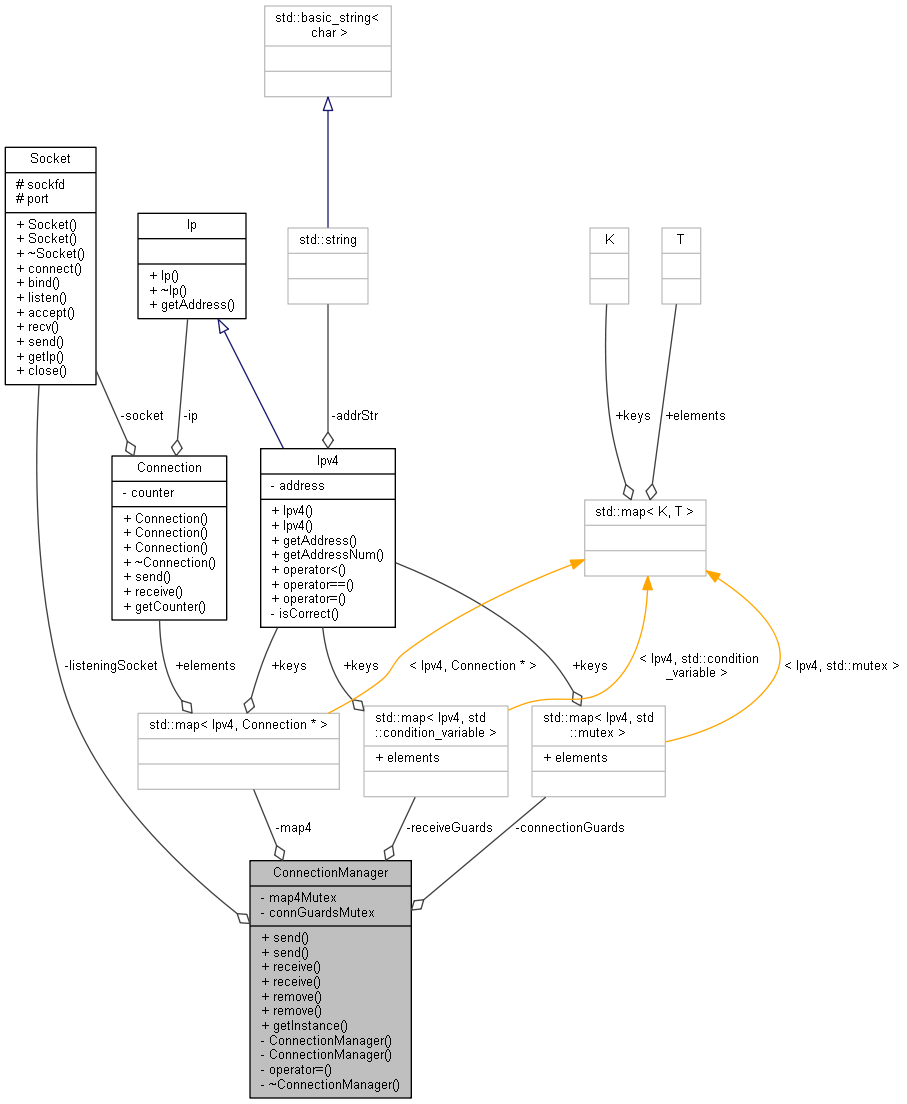
\includegraphics[width=\linewidth]{./images/classConnectionManager__coll__graph.png}
			\end{figure}
    
    \section{Serwer}
			
		\subsection{Opis}
			Serwer zarządza agentami, które kontrolują procesy na swojej platformie. Informacje o tym gdzie i co ma być zrobione dostaje z konsoli administratora. Kanałem komunikacyjnym z serwerem jest protokół LOTC działający na Ipv4 z wykorzystaniem mechanizmu gniazd sieciowych. \\
		
		\subsection{Reagowanie na zdarzenia}
			Zdarzeniami przychodzącymi do serwera mogą być polecenia z konsoli administratora, odpowiedzi od agentów lub zdarzenia wewnętrzne serwera np. time-out. Zdarzenia są obiektami z różnych klas typów zdarzeń dziedziczących po bazowej klasie zdarzeń, pojawiającymi się w kolejce zdarzeń. Zostają one obsłużone na podstawie mapy strategii i zdjęte z kolejki. Prawdopodobnie będzie około trzech różnych typów zdarzeń: komunikat z agenta, polecenie od administratora, zdarzenie wewnętrzne.
		
		\subsection{Moduły serwera}
			Serwer da się podzielić na kilka wyraźnych modułów: \\
			
			\begin{itemize}   
				\item Kontroler – przetwarza zdarzenia przychodzące z modułów i wykonuje lub zleca wykonanie odpowiednich metod w modułach. Odpowiada też za uruchomienie usług modułów szczególnie przy starcie serwera.
				\item Serwer klienta – odpowiada za komunikację z agentami. Serwer nawiązuje połączenie ze słuchającym agentem, wysyła polecenie, czeka na odpowiedź, otrzymaną odpowiedź wrzuca na kolejkę zdarzeń i zamyka połączenie. Może też nasłuchiwać na połączenia od agenta z wiadomością o zmianie statusu lub okresowym raportem.
				\item Serwer administratora – odpowiada za komunikację z konsolą administratora. Serwer czeka na polecenie od administratora, wrzuca na kolejkę zdarzeń i zwraca odpowiedź. Konsola administratora może sama nawiązać połączenie i wysłać polecenia, ale jeśli serwer ma po jakimś czasie odesłać raport, to konsola powinna też nasłuchiwać.
				\item Model – zbiór metod wywoływanych przez kontroler w celu realizacji wybranej strategi z mapy. Może też zawierać maszynę stanów i informacje o agentach.
			\end{itemize}
			Poszczególne moduły mogą pracować w osobnych wątkach lub procesach. Kontroler powinien być w wątku głównym. \\
			Model, o ile będzie zgłaszał jakieś zdarzenia (zapewne związane z upływem czasu), powinien mieć osobny wątek. Jeśli nie, to będzie wywoływany (jego metody) w tym samym wątku co kontroler. \\
			Serwer klienta, a właściwie każda jego instancja, powinien być w osobnym wątku. Wątki te powinny być tworzone wtedy gdy wyniknie to ze strategii działania. \\
			Serwer administratora również powinien być w osobnym wątku. \\
		
		\subsection{Komunikacja z konsolą i agentami}
			Komunikacja z konsolą i agentami odbywać będzie się poprzez protokół LOTC, przy wykorzystaniu modułu dostarczającego interfejs będący nakładką na protokół. \\
	    
	    \subsection{Diagram klas}
		    \begin{figure}[H]
				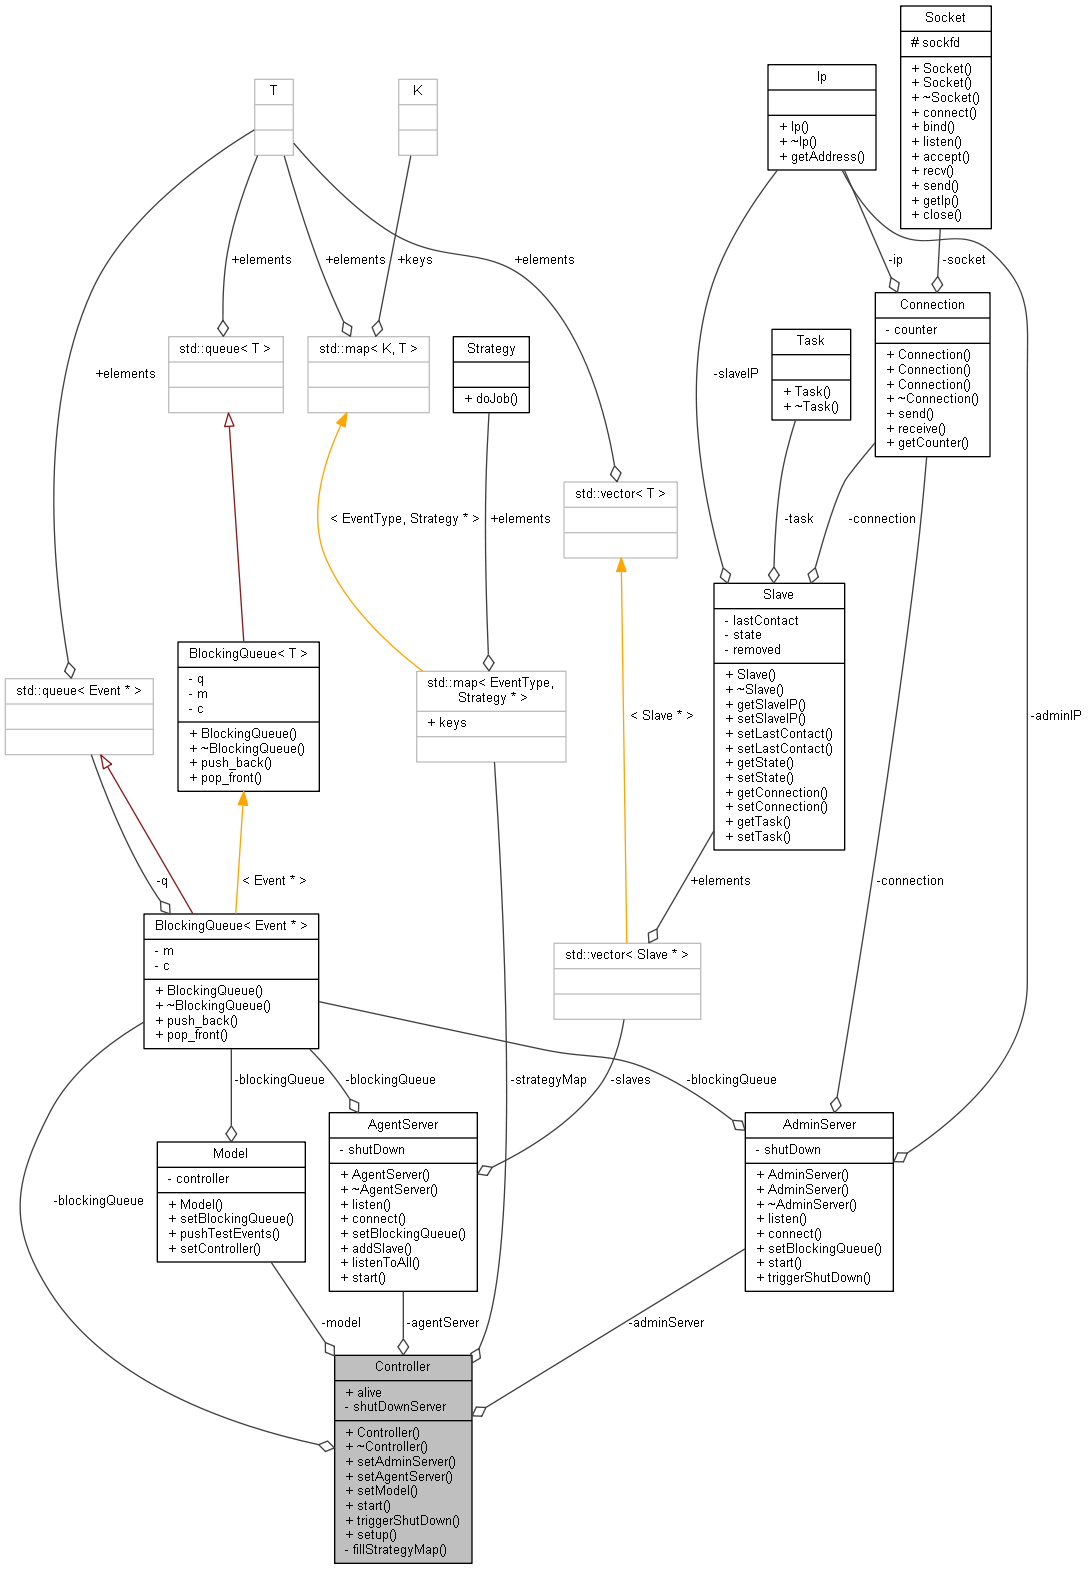
\includegraphics[width=\linewidth]{./images/classController__coll__graph.png}
		    \end{figure}		
    
    \section{Agent (klient LOTC)}
		\subsection{Opis}
			Agent to autonomiczny program zarządzający przydzielonymi przez serwer zadaniami. Agent zarządzający może: załadować/usunąć zadanie, uruchomić/zatrzymać/wznowić/zabić dany proces zgodnie z harmonogramem, podać dane statystyczne serwerowi. \\
			Agent komunikuje się z serwerem (protokołem działającym na IPv4) wykorzystując mechanizm gniazd sieciowych. \\
		
		\subsection{Zasady działania agenta}
			Agent po starcie łączy się z serwerem, następnie stale oczekuje na komunikaty wysyłane przez serwer. Po przyjściu komunikatu potwierdza jego otrzymanie a następnie analizuje jego treść według ustalonego protokołu. Potem wywołuje odpowiednią metodę w nowym wątku. Główny wątek dalej czeka na komunikaty od serwera, oraz wysyła raporty z wykonania innych wątków. \\
		
		\subsection{Zarządzanie zadaniami}
			Agent ma zdefiniowane metody, które będą wykonywane po otrzymaniu odpowiedniego polecenia z serwera. Lista poleceń: \\
			
			\begin{itemize}
				\item Załadowanie nowego zadania
				\item Usunięcie zadania
				\item Uruchomienie zadania
				\item Zabicie zadania
				\item Zatrzymanie wykonywania zadania
				\item Wznowienie wykonywania zadania
				\item Synchronizacja czasu
				\item Potwierdzenie żywotności 
			\end{itemize}

    	\subsection{Diagram klas}
		    \begin{figure}[H]
				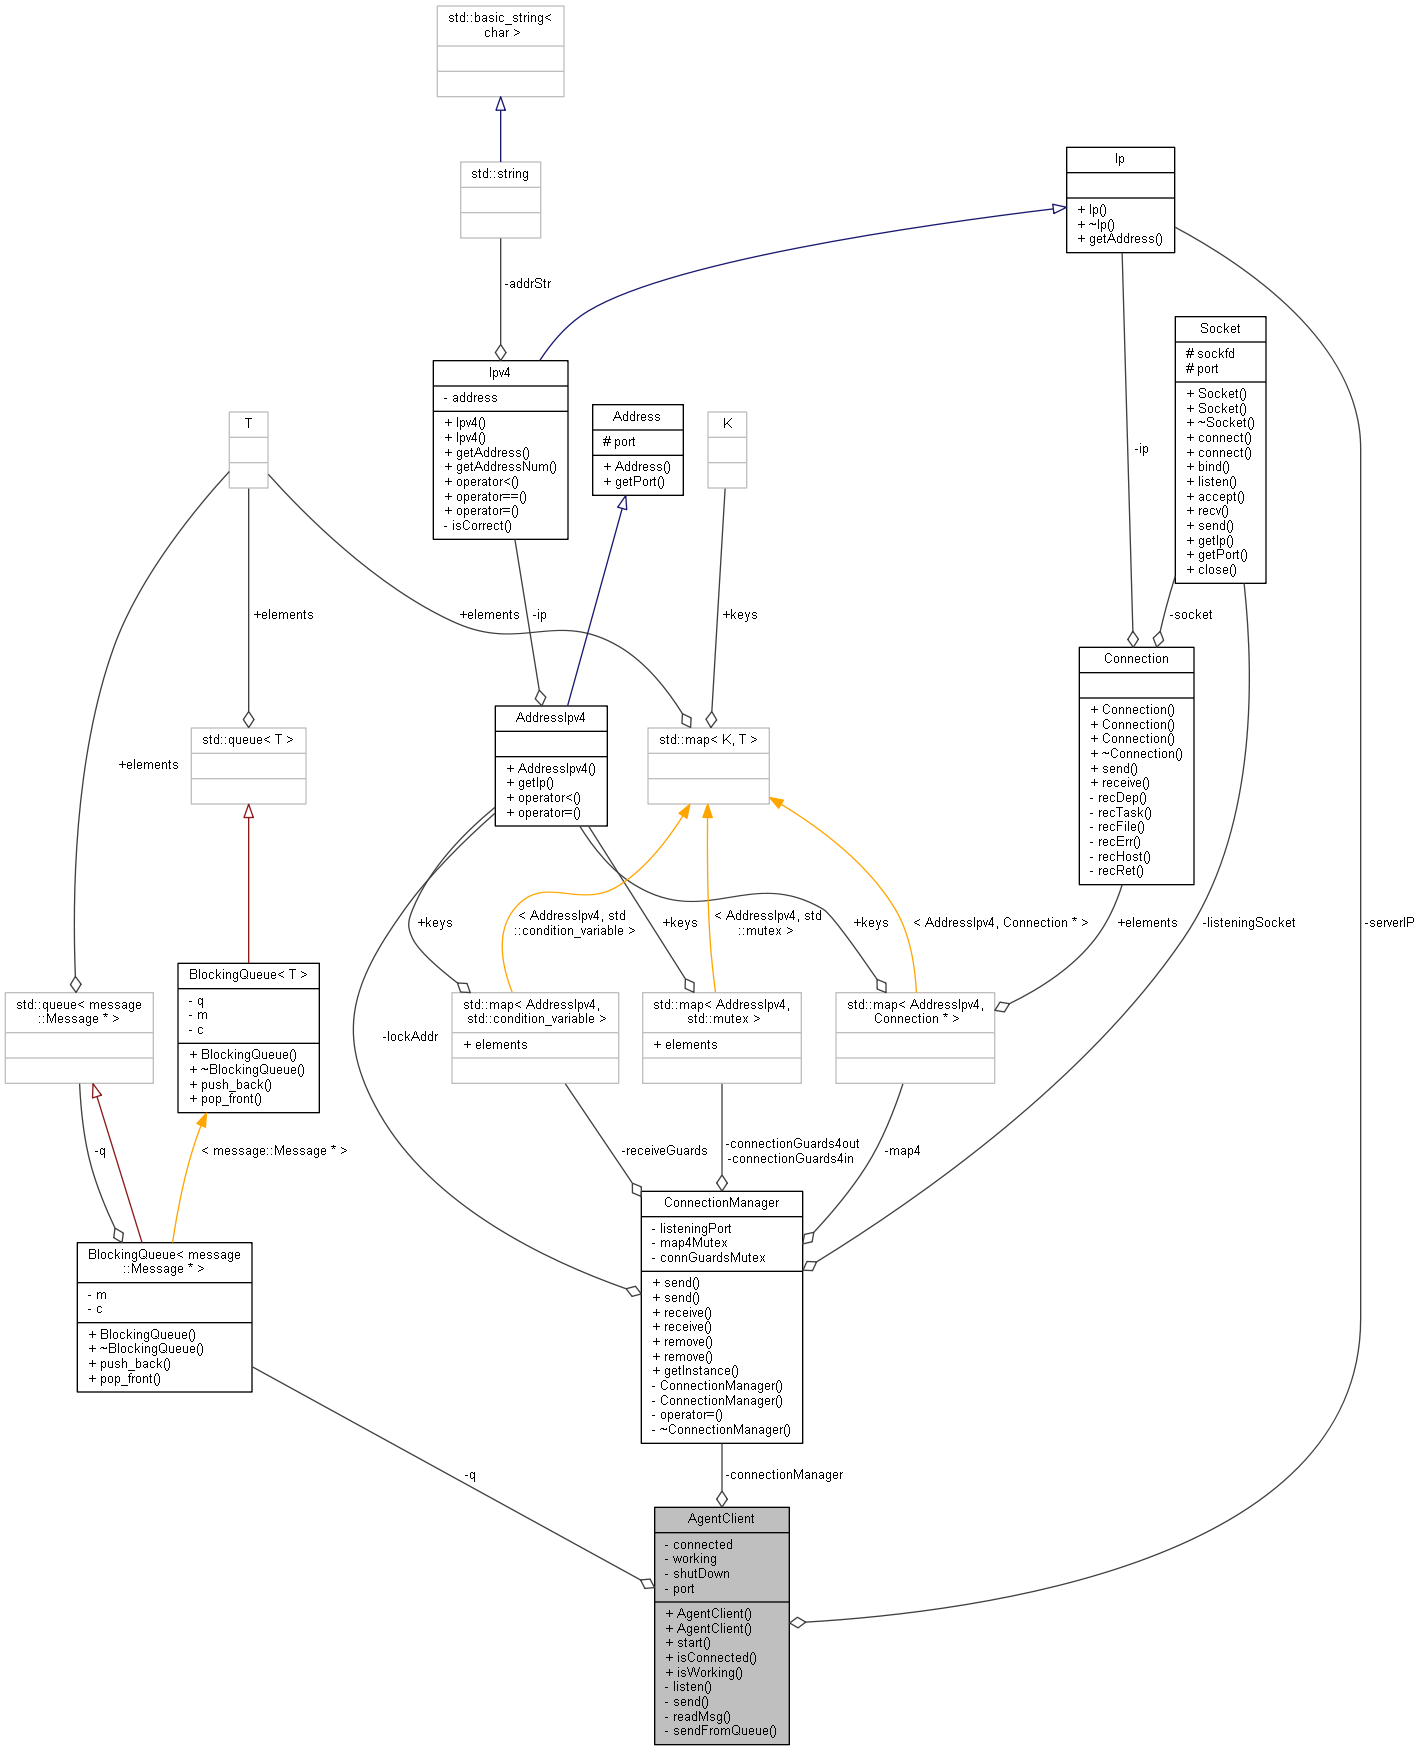
\includegraphics[width=\linewidth]{./images/classAgentClient__coll__graph.png}
		    \end{figure}
    
    \section{Konsola administratora}
		\subsection{Opis}
			Konsola administratora stanowi interfejs, który umożliwia użytkownikowi (administratorowi)  sterowanie systemem komunikacji zarządzania rozproszonymi procesami. Poprzez wysyłanie odpowiednich komend, użytkownik powinien mieć możliwość pełnej konfiguracji systemu, wydawania konkretnych poleceń związanych z pracą systemu oraz otrzymywania informacji zwrotnych o statusie całego systemu. Informacje zwrotne można wykorzystać do generowania raportów. Dodatkowo konsola administratora powinna zadbać o poprawność wprowadzanych komend i danych, a także sprawdzać parametry komunikatów otrzymywanych z sieci.
		
		\subsection{Komunikacja z serwerem}
			Komunikacja konsoli administratora z serwerem odbywa się dwustronnie, tj. do serwera są wysyłane komendy i polecenia, a od niego otrzymywane są raporty i informacje zwrotne, a także komunikaty o błędach. Wymaga to ciągłego nasłuchiwania komunikatów z serwera (informację można dostać w dowolnym momencie) przy jednoczesnym rozpoznawaniu komend wydanych przez użytkownika i, po sprawdzeniu ich poprawności, wysłaniu ich na serwer. Wymaga to powołania do pracy dwóch wątków (nasłuchującego i wysyłającego).
		
		\subsection{Sprawdzanie poprawności}
			W programie konsoli administratora będzie sprawdzana poprawność wpisywanych komend, ewentualnych argumentów programu podawanych z linii poleceń (do czego to będzie potrzebne i czy w ogóle?) oraz parametrów komunikatów odebranych z sieci, w celu uniknięcia błędów związanych z działaniem systemu lub celowego złośliwego działania i ataków na system. Na przykład gdy informacje zwrotne z serwera będą zawierały nieprawidłowy identyfikator węzła/procesu zostaną zignorowane, a próba powtórzona.
		
		\subsection{Komendy}
			Komendy wydawane w konsoli administratora powinny umożliwiać:
			
			\begin{itemize}   
				\item Dodanie/usunięcie/wstrzymanie/wznowienie zadania
				\item Nadanie zadaniu priorytetu podczas dodawania
				\item Definiowanie kolejności następowania zadań
				\item Oznaczenie zadania jako gotowego do przetwarzania
				\item Dodanie/usunięcie agenta
				\item Żądanie otrzymania raportu o pracy systemu (jednorazowo bądź cyklicznie)
			\end{itemize}
		
		\subsection{Raporty}
			Konsola administratora, dzięki otrzymywaniu raportów z serwera, w tym raportów cyklicznych, może generować zbiorczy raport z całej pracy systemu (przez określony czas lub do zakończenia pracy) w oddzielnym pliku. Format tych raportów pozostaje do ustalenia (jakie informacje, kiedy, jak często, w jakiej formie to przedstawić).
			
    	\subsection{Diagram klas}
		    \begin{figure}[H]
				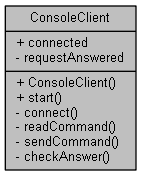
\includegraphics[width=\linewidth]{./images/classConsoleClient__coll__graph.png}
		    \end{figure}  
		      
    \section{Przypadki użycia}
        Aby zmniejszyć objętość przypadków użycia, a zwłaszcza scenariuszy alternatywnych, powtarzające się, schematyczne działania zostaną opisane osobno w sposób ogólny.                    
        
        \subsection{Wysłanie polecenia}
            Proces zlecenia wykonania jakiegoś działania wygląda następująco:
            
			\begin{enumerate}
	            \item Zlecającemu wysyła polecenie i czeka na odpowiedź
	            \item Odbiorca wysyła potwierdzenie odebrania polecenia
	            \item Odbiorca wykonuje polecenie
	            \item Odbiorca wysyła komunikat o sukcesie/porażce
	            \item Zlecający, po otrzymaniu komunikatu o sukcesie/porażce wysyła potwierdzenie otrzymania
	            \item Zlecający podejmuje dalsze działania 
			\end{enumerate} 
		 
        \subsection{Błędy}
            Wystąpienie w trakcie wykonywania polecenia błędu zawsze wiąże się z następującym schematem działania:
            
            \begin{enumerate}
	            \item Wykonawca zgłasza zlecającemu porażkę w wykonaniu czynności
	            \item Wykonawca wysyła zlecającemu stosowny komunikat ERR określający przyczynę błędu
	            \item Zlecający wysyła potwierdzenie otrzymania komunikatu o błędzie
	            \item Zlecający podejmuje dalsze działania  
            \end{enumerate}
            
            \paragraph{Błędy protokołu:}
            
            \begin{itemize}
	            \item Za długi/za krótki nagłówek
	            \item Zabronione wartości pól 
            \end{itemize}
            
            \paragraph{Błędy logiki:}
            
            \begin{itemize}
	            \item Dodawanie istniejących już zadań/plików/agentów
	            \item Usuwanie nieistniejących zadań/agentów
	            \item Oznaczenie jako gotowych nieistniejących zadań
	            \item Uruchamianie niegotowych zadań
	            \item Zabicie nieuruchomionych zadań
	            \item Zatrzymywanie nieuruchomionych zadań
	            \item Wznowienie niezatrzymanych zadań
	            \item Ustalanie kolejności wykonywania nieistniejących zadań
	            \item Ustalanie kolejności wykonywania zadań oznaczonych jako gotowe
            \end{itemize}
            
		\subsection{Przekroczenie czasu oczekiwania na odpowiedź}
            Jeśli jedna strona nie odpowiada, strona oczekująca próbuje kilkukrotnie nawiązać komunikację komendą PING (protokołu LOTC). Jeśli uzyska odpowiedź, powtarza polecenie na które nie otrzymała odpowiedzi jeśli nie, dalsze działania zależą od tego, kim jest strona oczekująca:
            \begin{itemize}
	            \item Agent: kontynuuje wykonywanie przydzielonych już zadań
	            \item Serwer: oznacza agenta jako nieresponsywnego, przekazuje zadania tego agenta innym agentom
	            \item Konsola: powiadamia użytkownika o utracie łączności z serwerem
            \end{itemize}
            Ponadto strona oczekująca okresowo próbuje nawiązać komunikację za pomocą komendy PING.
            
        \subsection{Przypadek użycia: obsługa zadań i agentów}
            \begin{enumerate}
	            \item Administrator wydaje polecenie dodania/usunięcia/wykonania/zabicia/wstrzymania/wznowienia zadania, oznaczenia zadania jako gotowego, ustalenia kolejności wykonywania zadań lub dodania/usunięcia agenta
	            \item Konsola przesyła odpowiedni komunikat serwerowi
	            \item Serwer aktualizuje stan zadań/agentów zgodnie z poleceniem
	            \item Serwer przesyła konsoli odpowiedni raport i aktualizuje strategię wykonywania zadań
	            \item Konsola wyświetla raport administratorowi
            \end{enumerate}
        
        \subsection{Przypadek użycia: żądanie raportu}
            \begin{enumerate}
	            \item Administrator wydaje żądanie raportu
	            \item Konsola przesyła odpowiedni komunikat serwerowi
	            \item Serwer zbiera niezbędne dane, odpytując agentów jeśli to konieczne
	            \item Serwer przesyła konsoli odpowiedni raport
	            \item Konsola wyświetla raport administratorowi
            \end{enumerate}
    
	\section{Sposób testowania aplikacji}
		Testowanie działania systemu odbywać się będzie etapami: \\
		\begin{enumerate}
		    \item Kompilacja i wykrycie błędów składniowych poszczególnych modułów
		    \item Testy jednostkowe dla poszczególnych metod klas (tam, gdzie to zasadne)
		    \item Testy integracyjne z wykorzystaniem pluginu do Wiresharka sprawdzające poprawność wysyłanych komunikatów i wywołań powiązanych z nimi metod
		    \item Uruchomienie skryptu do konsoli administratora symulującego przypadki użycia
	    \end{enumerate}
	    
	    Wykorzystanie metodykę zwiną i iteracyjnego modelu wytwarzania oprogramowania pozwoli na przeprowadzenie testów już po implementacji minimum funkcjonalności systemu. Testy będą stopniowo rozszerzane wraz z rozbudową systemu.

	\section{Sposób  demonstracji rezultatów}
		Demonstracja rezultatów będzie się opierała na realizacji wybranych (lub wszystkich) przypadków użycia przy wykorzystaniu napisanego wcześniej skryptu testującego.
		
	\section{Wnioski}
        \subsection{Tomasz Jakubczyk - wnioski z testowania}
            Niezaprzeczalnie poprawnie działa kolejka blokująca BlockingQueue. Jest to bardzo ważny element projektu, gdyż zapewnia niezawodną synchronizację wątków. Bez tego nie było by szans, żeby coś działało. \\
            Każdy z modułów, czyli serwer, konsola, agent i protokół, same z siebie wydają się działać poprawnie, jednak testowanie wykazało, że moduły te zapałały do siebie gorącą nienawiścią. \\
            Ponadto wykorzystywane kompilatory g++ i biblioteki obsługujące standard c++11 i c++14 wykazują się różnymi dziwnymi zachowaniami. O ile kompilacja i linkowanie przebiega pomyślnie, to nie można powiedzieć, że wykonanie programów takie jest. \\
            Na Ubuntu występuje błąd \\
            \texttt{ *** buffer overflow detected ***: terminated } \\
            wydaje się, że jest to wina bibliotek dystrybucji Linuxa. \\
            Inne problemy występują pod Cygwinem, który teoretycznie powinien być zgodny z Linuxem. Tam wydaje się, że Istnieją pewne ograniczenia co do otwierania i zamykania gniazd. Objawia się to, niemożliwością powtórnego nawiązania połączenia. Nie da się też wykluczyć, że powyższe błędy są związane z testowaniem poszczególnych, modułów aplikacji naraz na jednym komputerze bez ustawionych maszyn wirtualnych. Wydaje się, że biblioteki socket nadal są niedopracowane i zawierają błędy. \\
            Nie mniej udaje się wykonywać programy aplikacji LOTC na Linux Arch, bez wyżej wymienionych błędów. \\
            Mimo, że prawie od samego początku projektu zaczęliśmy testować protokół aplikacji, to i tak pod koniec, okazało się, że w połączeniu z pozostałymi częściami aplikacji wszystko nagle przestało działać. Być może było to spowodowane zbyt słabym opisaniem metod publicznych klas protokołu. W trakcie integrowania ze sobą modułów wyszły na jaw różne nieporozumienia co do działania protokołu. Być może przy protokole powinno pracować więcej osób, albo najlepiej wszyscy, ale to by oznaczało wchodzenie sobie w drogę. \\
            Jeśli jeszcze raz miał bym robić ten projekt, to wstępnie zarządził bym, żeby każdy napisał własną obsługę gniazd do przesyłania komunikatów protokołu i wtedy dużo łatwiej było by wykrywać błędy, bo wyraźnie były by widoczne wizje działania komunikacji sieciowej poszczególnych programistów i dało by się ich w porę naprostować. \\
            Testowanie okazało się też niesamowicie czasochłonne i nieprzyjemne.\\
            Mimo usilnych starań nie udało się przekonać członków zespołu do napisania odpowiedniej liczby testów jednostkowych i postało ich zaledwie kilka.\\
            Zostało napisanych kilka skryptów testowych, ale raczej w niczym one nam nie pomogły, a próby doprowadzenia ich do działania na niektórych maszynach i systemach zajęły sporo czasu. Oczywiście niezwykle przydatne okazały się ogromne ilości komunikatów debugowania oraz GDB pozwoliło szybko znaleźć kilka poważnych błędów, ale nie wszystkie. \\
            GDB wykazuje się złym zachowaniem, jeśli w programie zwracane są wyjątki, które nie mają zakończyć programu. \\
            Być może powinno się wyznaczyć jedną osobę, która zajmowała by się tylko testowaniem tego co inni napisali. \\   
        \subsection{Tomasz Jakubczyk - opis doświadczeń z projektu}
Po pierwsze lepiej dobierać współpracowników. \\
Zwykle ten obowiązek spada na head hunterów, a przynajmniej można zobaczyć CV. Niestety, osoby preferowane na członków projektu postanowiły nie zapisać się na przedmiot TIN. Nie uzyskałem też zgody na realizowanie projektu w mniejszym zespole, co niewątpliwie dało by lepszy efekt. \\
Bardzo zauważalny okazał się brak środków nacisku na członków zespołu. Niektórzy członkowie mimo napomnień odkładali pisanie projektu, a na końcu zamiast wziąć się w garść i zarwać trzy noce odpuścili sobie zupełnie. Być może częściowo ponosi za to winę okres świąteczny, zalew kolokwiami i innymi projektami przez czas trwania projektu od prezentacji wstępnej do terminu oddania. \\
Być może jeśli cały projekt byłby zadany już w pierwszym lub drugim tygodniu semestru, kiedy jest jeszcze dużo czasu i termin oddania byłby gdzieś w pierwszej połowie semestru, przebieg projektu byłby zgoła inny. Nie widzę też żadnego dobrego uzasadnienia, czemu tak by nie miało być, bo wiedzę potrzebną do zakodowania aplikacji albo w większości już posiadaliśmy, albo i tak musieliśmy doczytać bezpośrednio ze źródeł (internetu). \\ \\
Problemem okazało się też zbyt mało precyzyjne opisanie szczegółów implementacji protokołu w dokumentacji wstępnej. Uważam, że opis pól komunikatów był niewystarczający. Powinniśmy byli napisać jak dokładnie będziemy wykorzystywać gniazda, z pewnością oszczędziło by to wiele czasu przy próbach integracji modułów aplikacji. \\ \\
Okazało się, że niektórzy członkowie mają skłonność do rzadkiego commitowania swoich postępów na githuba, co utrudniało kontrolę sytuacji. Przydało by się jakieś oprogramowanie do podglądania, czym właśnie zajmują się członkowie zespołu.
Niezwykle przydatny okazał się komunikator Skype w fazie integracji i debugowania aplikacji. Pozwoliło to szybko zorientować się w sytuacji co do projektu i nakierować tok prac na właściwe tory. \\
Dla odmiany Facebook nie okazał się zbyt dobrym sposobem komunikacji, chociaż mogło to wynikać z tego którzy członkowie zespołu wykorzystywali go do komunikacji. Komunikacja przez Facebooka prowadziła często do tego, że pytania bądź polecenia
pozostawały bez odpowiedzi. Może być to też związane ze zbyt dużym natłokiem informacji na Facebooku. \\
Zauważalna była duża rozbieżność w umiejętnościach programistycznych członków zespołu. Jest to zapewne związane z tym, że program studiów informatyki na Wydziale Elektroniki Politechniki Warszawskiej przewiduje stanowczo za mało
godzin poświęconym nauce języków programowania. \\
Testowanie regresyjne oraz integracyjne powinno być przeprowadzane co najmniej raz w tygodniu, niestety, niektórzy członkowie aż do końca projektu nie napisali nic co mogło by się do tego nadawać. \\
Sądzę, że wprowadziliśmy zbyt rozbudowaną strukturę logiczną projektu, który tego na prawdę nie wymagał i przez to nie starczyło czasu na pełne zrealizowanie projektu. Jeśli projekt zostałby napisany strukturalnie w języku c przez jedną
osobę, to wyszło by to dużo prościej, dużo szybciej, zostały by zrealizowane wszystkie założenia projektowe i debugowanie okazało by się dużo prostsze. \\
Ubolewamy, też nad tym, że nie udało się napisać pluginu Wiresharka do podglądania komunikacji sieciowej, jednak w naszym przypadku dużo by nie pomógł i uznaliśmy, że w zbyt ograniczonym czasie potrzeba zająć się raczej usuwaniem błędów
krytycznych wywołania programu. \\
W ostatnich dniach projektu byliśmy o krok od uzyskania działającego jednocześnie IPv4 i IPv6, jednak zabrakło na to czasu i w ogromie innych problemów musieliśmy zadowolić się działającym IPv4. Gdyby na początku projektu klasa Ip nie była
by klasą wirtualną po której dziedziczą Ipv4 i Ipv6, to niewątpliwie to by się nam udało. Niestety na chwilę obecną Ipv6 jest tylko częściowo zrealizowane w kodzie. \\
Już tydzień przed końcem projektu zorientowaliśmy się, że raczej nie ma szans na realizacje synchronizacji zegarów przez pobranie z serwera NTP, niemniej został napisany kod do protokołu który może bez problemu obsługiwać tą opcję. \\
Okazało się też, że i tak testujemy naszą aplikację w jednym środowisku i sens tego jest znikomy. \\
        \subsection{Andrzej Roguski}
            Jeśli miałbym wskazać największe gwoździe w trumnie projektu, byłyby nimi faza projektowania i testowania. \\
            \\
            Znaczącym problemem okazała się rzecz prozaiczna - aplikacja docelowo mająca działać na wielu hostach, była testowana na pojedynczej maszynie. \\
            Aby w ogóle umożliwić uruchomienie na jednym hoście serwera, konsoli i agentów, moduł komunikacyjny musiał poradzić sobie z przetwarzaniem komunikatów nie na podstawie samych adresów IP, ale także i portów. \\
            Każdy moduł musiał nasłuchiwać na innym porcie. Serwer musiał też po porcie rozpoznawać rozmówców - a ten domyślnie był losowany. Przypisanie konkretnych portów wyjściowych prowadziło do błędów funkcji związanych z socketami, mimo użycia \texttt{SO\_REUSEADDR} - i na tej zasadzie bardzo duża część czasu poświęcona została na walkę z funkcjonalnością niezwiązaną z samym zadaniem, który to czas mógłby zostać wykorzystany na pisanie testów, implementację obsługi IPv6 czy stworzenie modułu Wireshark. \\
            Co gorsza, z nieznanych nam przyczyn aplikacje inaczej zachowywały się (czyt. działały bądź nie) u różnych osób - mimo środowisk teoretycznie spełniających wymogi dotyczące kompilacji i uruchomienia. \\
            \\
            Mam też wrażenie, że wielu problemów można by uniknąć dzięki większej liczbie spotkań projektowych i większej aktywności zespołu przed przystąpieniem do "prac głównych". Jeszcze na etapie integracji pokutowały nieporozumienia odnośnie działania poszczególnych modułów albo głupie przeoczenia oczywiste z perspektywy programisty-odbiorcy danej funkcjonalności. \\
            \\
            Na pewno nie pomogła znikoma aktywność aż połowy zespołu - mimo usilnych nalegań teamleadera, połowa(!) modułów powitała nowy rok w stanie niemal dziewiczym, co doprowadziło do panicznego wyścigu z czasem w ostatnim tygodniu przerwy świątecznej. Dodając do tego niezrozumiałe różnice w działaniu aplikacji, pod koniec prac tylko ja miałem możliwość testowania aplikacji, a Tomek dokładną znajomość kodu serwera, konsoli i agenta, co skutkowało tym, że żaden z nas nic sensownego nie mógł w rozsądnym czasie osiągnąć. Pierwotny zamysł przydzielania sił zespołu tam, gdzie jest to potrzebne runął w gruzach.



	\section{Wkład}
	\subsection{Podział prac}
	    \begin{tabular}{ l | l }
		    \textbf{Osoba odpowiedzialna} & \textbf{Zadania} \\
		    \hline
		    Tomasz Jakubczyk  & Teamleader, serwer  \\
		    Eryk Ratyński  & Agent  \\
		    Andrzej Roguski  & Protokół, klient NTP, plugin Wireshark, dokumentacja \\
		    Kacper Stachyra & Konsola administratora \\
		\end{tabular}
		
	\subsection{Praca przy zadaniach}
        \begin{tabular}{ l | l }
		    \textbf{Osoba} & \textbf{Zadania} \\
		    \hline
		    Tomasz Jakubczyk  & Teamleader, serwer, konsola, agent, testowanie  \\
		    Eryk Ratyński  & Agent  \\
		    Andrzej Roguski  & Protokół (IPv4), dokumentacja, testowanie \\
		    Kacper Stachyra & Konsola administratora \\
		\end{tabular}
		
	\subsection{Czas}
        \begin{tabular}{ l | l }
		    \textbf{Osoba} & \textbf{Zadania} \\
		    \hline
		    Tomasz Jakubczyk  & około 100 h  \\
		    Eryk Ratyński  & około 25 h  \\
		    Andrzej Roguski  & około 100 h \\
		    Kacper Stachyra & około 25 h \\
		\end{tabular}
    
    \subsection{Statystyki z GitHuba}
    \textbf{Statystyki są niedokładne - GitHub po 02.01.2016 zaczął traktować commity Andrzeja Roguskiego (anrog) jako anonimowe i nie wliczał ich do statystyk użytkownika.}
		    \begin{figure}[H]
				\includegraphics[width=\linewidth]{./images/github.png}
			\end{figure}
		
\end{document}
